\chapter{Multivariate Analysis}\label{cha:mva}

In this chapter a method for applying boosted decision trees to the $\Httll$ analysis is presented.
First, the event selection of the cut-based analysis (CBA) is modified to allow for more inclusive regions.
Afterwards the BDT training and evaluation scheme is introduced in \cref{sec:mva:sets,sec:mva:kfold-xval},
which is then applied to the optimization of the hyperparameters and set of observables used for the BDTs (\cref{sec:mva:optimization}).
The chapter closes with evaluation the modeling of the chosen observables and BDT output distributions.

\section{Event Selection}\label{sec:mva:event_selection}

The boosted decision trees could be used to separate signal and background events in the VBF and boosted category as defined in \cref{sec:event_selection:categorization},
to increase the sensitivity.
However, a lot of signal and background events are already discarded by all the thresholds set on observables in the preselection and categorization step.
These thresholds were used to select the signal topology and to suppress background contributions.
But BDTs offer an alternative way to separate between signal and background events, which is more powerful because no event is
discarded.
Therefore, some thresholds which are used to suppress background are removed to increase the signal yield.
The increased number of background events is handled by the BDTs, so that in the end the sensitivity should increase.
Nevertheless, removing too many thresholds will result in the opposite effect, because the training of decision trees
focuses first on background processes, which are easy to separate from the signal.
Because the depth of the decision trees is limited, not the full splitting potential for background events which are harder to separate from signal events may be reached.
Thus, requirements on observables which remove huge amounts of background while increasing the signal-to-background ratio are not modified.

Only thresholds after the requirement of opposite charge of the two decay leptons (Cut~6) are considered for removal.
The requirements on the dilepton mass, missing transverse energy, and missing transverse energy for high-$\pt$ objects
(Cut~7, Cut~9, Cut~10) are kept, because they suppress a large amount of $\Zgammall$ background without removing a lot of signal
events.
Furthermore, the threshold on the transverse momentum of the leading jet (Cut~8) is also kept, since it helps to select
both the VBF and boosted topology.
The thresholds on the momentum fractions $x_{1,2}$ and the angular differences
$\detall$ and $\drll$ (Cut~11, Cut~12, Cut~13) are removed, since they remove a sizable amount of signal events without
increasing the signal-to-background ratio.
The requirement on the collinear mass (Cut~14) has to be kept, otherwise the orthogonality to the $H \to WW$ analysis would be violated.
Since the output of the missing mass calculator, $\mmc$, will be used as an input variable for the BDTs, only events can be used where
the MMC mass reconstruction algorithm did converge.
Thus, Cut~15 is also kept.
Events containing $b$-jets are still rejected (Cut~16), since this provides a good discrimination against the
single-top and $t\overline{t}$ background.

In the definition of the VBF category only the requirement that the two jets need to occupy different hemispheres (Cut~2V)
is dropped, because for a strongly boosted system the jets can also be in the same hemisphere.
The boosted category is not directly modified, but affected by the change in the VBF category, because a veto on events which pass the VBF selection is used.

Because the thresholds are changed, the pre-fit normalization factors which are discussed in \cref{sec:background_estimation:normalization}
need to be recalculated.
The normalization factors are calculated both in the modified VBF and boosted category.
The results are shown in \cref{tab:mva:event_selection:NF}.
In the following these normalization factors for the individual categories are used.

\begin{table}[htpb]
    \centering
    \caption{Pre-fit normalization factors for the multivariate analysis.}\label{tab:mva:event_selection:NF}
    \begin{tabular}{lccc}
        \toprule
        Selection        & $Z \to \ell\ell$ & $Z \to \tau\tau$ & Top \\ \midrule
        VBF category     & $0.97 \pm 0.15$ & $1.07 \pm 0.15$ & $1.14 \pm 0.03$ \\
        Boosted category & $1.04 \pm 0.03$ & $1.05 \pm 0.03$ & $1.08 \pm 0.01$ \\
        \bottomrule
    \end{tabular}
\end{table}

%The event yields after each threshold of the modified event selection can be found in \cref{tab:mva:event_selection:cutflow}.
%TODO cutflow table

Furthermore, the categories are split into subcategories based on the flavour combination of the final state leptons.
The SF category holds events where the final state leptons have the same flavour ($ee$ and $\mu\mu$).
Events with $e\mu$ and $\mu e$ are sorted into the DF (\emph{different flavour}) category.
This increases the sensitivity and leads to a better training of the BDT, since those regions have a different background composition and signal-to-background ratio.
The event yields in each subcategory are given in \cref{tab:mva:event_selection:yields}.

For training BDTs it is also important that the number of simulated events is not too low.
The number of simulated events for each subcategory is shown in \cref{tab:mva:event_selection:rawyields}.
The training statistics for the ggF and VBF signal process are very good.
Other signal processes are not used in the training, as discussed in \cref{sec:mva:optimization}.
Also most background processes have at least $1000$ simulated events left.

There are around \SI{50}{\percent} more signal events in the VBF and boosted category of the multivariate analysis than
for the cut-based analysis.
However, the background yields also increase by a factor of 3 and 1.5 in the VBF and boosted category, respectively.
This reduced the signal-to-background ratio of \SI{3.7}{\percent} and \SI{1.1}{\percent} the VBF and boosted category
of the cut-based analysis to \SI{2.2}{\percent} and \SI{0.97}{\percent}, respectively.

\begin{sidewaystable}
    \centering
    \caption{Expected event yields for the different signal and background processes in the subcategories of the
             multivariate analysis with a combined 2016 and 2016 dataset of $\SI{36.1}{\invfb}$.
             Normalization factors are applied on the top-quark, $\Zll$, and $\Ztautau$ background.
             Only statistical uncertainties are shown.}\label{tab:mva:event_selection:yields}
    \begin{tabular}{@{}l@{}
                    S[separate-uncertainty,table-figures-uncertainty=1]
                    S[separate-uncertainty,table-figures-uncertainty=1]
                    S[separate-uncertainty,table-figures-uncertainty=1]
                    S[separate-uncertainty,table-figures-uncertainty=1]
                    @{}}
        \toprule
        \multirow{2}{*}{Process} & \multicolumn{2}{c}{VBF category}      & \multicolumn{2}{c}{Boosted category} \\ \cmidrule{2-5}
                            & {SF}             & {DF}              & {SF}               & {DF}                  \\ \midrule
        ggF $\Htt$          &   3.61 \pm  0.13 &    8.85 \pm  0.21 &   33.22 \pm   0.36 &   53.86 \pm  0.47     \\
        VBF $\Htt$          &   9.04 \pm  0.08 &   17.01 \pm  0.11 &    7.16 \pm   0.07 &   10.69 \pm  0.09     \\
        WH  $\Htt$          &   0.09 \pm  0.02 &    0.17 \pm  0.03 &    2.82 \pm   0.14 &    4.43 \pm  0.18     \\
        ZH  $\Htt$          &   0.02 \pm  0.01 &    0.10 \pm  0.02 &    1.67 \pm   0.08 &    2.11 \pm  0.10     \\
        ttH $\Htt$          &   0.07 \pm  0.04 &    0.32 \pm  0.10 &    1.94 \pm   0.18 &    3.52 \pm  0.24     \\ \cmidrule{1-5}
        Fakes               &  73    \pm 13    &  293    \pm 16    &  713    \pm  36    &  987    \pm 31        \\
        Top                 &  74    \pm  4    &  251    \pm  7    &  511    \pm  10    & 1368    \pm 16        \\
        Diboson             &  22.30 \pm  0.91 &   64.58 \pm  1.92 &  306.60 \pm   4.22 &  671    \pm 14        \\
        $\Zgammall$         & 211    \pm 90    &   10.52 \pm  3.72 & 1082    \pm 101    &   88    \pm 11        \\
        $\Zgammatt$         & 187    \pm  9    &  574    \pm 17    & 2608    \pm  37    & 4365.83 \pm 42        \\
        $\HWW$              &   7.47 \pm  0.36 &   13.60 \pm  0.47 &   24.17 \pm   0.91 &   40.79 \pm  1.28     \\ \cmidrule{1-5}
        Total signal        &  12.83 \pm  0.16 &   26.46 \pm  0.26 &   46.80 \pm   0.44 &   74.61 \pm  0.58     \\
        Total background    & 575    \pm 92    & 1207    \pm 25    & 5244   \pm 114    & 7521     \pm 58        \\ \bottomrule
    \end{tabular}
\end{sidewaystable}

\begin{sidewaystable}
    \centering
    \caption{Number of simulated events for the different signal and background processes in the subcategories of the
             multivariate analysis.}\label{tab:mva:event_selection:rawyields}
    \begin{tabular}{@{}l@{}SSSS@{}}
        \toprule
        \multirow{2}{*}{Process} & \multicolumn{2}{c}{VBF category}      & \multicolumn{2}{c}{Boosted category} \\ \cmidrule{2-5}
                            & {SF}  & {DF}  & {SF}   & {DF}   \\ \midrule
        ggF $\Htt$          &  1137 &  2614 &  11111 &  17433 \\
        VBF $\Htt$          & 16613 & 31003 &  13304 &  19654 \\
        WH  $\Htt$          &    18 &    34 &    550 &    835 \\
        ZH  $\Htt$          &     6 &    29 &    480 &    611 \\
        ttH $\Htt$          &    36 &    94 &    659 &   1367 \\ \cmidrule{1-5}
        Fakes               &   786 &  3130 &   6602 &  17807 \\
        Top                 &   525 &  1739 &   3918 &  10324 \\
        Diboson             &  2633 &  7007 &  32222 &  66007 \\
        $\Zgammall$         &  1447 &   168 &  11463 &   1233 \\
        $\Zgammatt$         &  3533 &  9142 &  57313 &  90378 \\
        $\HWW$              &  1026 &  1775 &   1418 &   2210 \\ \cmidrule{1-5}
        Total signal        & 17810 & 33770 &  26104 &  39900 \\
        Total background    &  9950 & 22961 & 112936 & 187959 \\ \bottomrule
    \end{tabular}
\end{sidewaystable}


\section{Model Selection and Assessment}\label{sec:mva:sets}

Boosted decision trees need some data where the correct classification is known for the training.
This knowledge can only be provided by simulated events.
Ideally, all simulated events are used for the training, because a higher number of training events
leads to a better performing model.
However, the BDT hyperparameters and input variables need to be optimized.
A way of estimating the performance of a specific BDT is needed.

The performance of a BDT cannot be measured with the same set of simulated events which was also used
to train this BDT, because this would introduce a bias.
An independent set of simulated events, the so-called \emph{validation} set, needs to be used to estimate
the performance of the BDT\@.

In high-energy physics analyses simulated events are needed for background estimation.
For this neither the events from the training set and validation set can be used, because this would again
introduce a bias.
A third set of simulated events, the \emph{test set}, is needed for the background estimation,
which has to be independent from the two other sets.

The amount of simulated events is not unlimited, and especially the uncertainty of the measurement (where the test set is used)
depends on the number of simulated events.
On the other side the training statistics should also not be chosen to small, so that the performance of the BDT
does not suffer.
Because the training, validation, and test set need to be independent of each other there is always a tradeoff
between the contributions to those sets.
In a typical splitting scheme \SI{50}{\percent} of the events are used for the training set, \SI{25}{\percent} for the validation set, and
\SI{25}{\percent} for the test set~\cite{Hastie2009}.

\section{$k$-fold Cross-Validation}\label{sec:mva:kfold-xval}

The $k$-fold cross-validation approach~\cite{Hastie2009} is one solution to improve the statistics for the training, validation, and
test set.
Here the full set of simulated events is split into $k$ slices of equal size.
Usual values for $k$ are 5 or 10~\cite{Hastie2009}.
In this analysis $k=10$ is used.
There should be no or only a very small dependence on the choice of $k$.
The splitting is done with the help of a random number, which is generated once for each event.

Now $k$ different BDTs are trained, each using $k-2$ slices for training, one slice for validation, and one slice for testing.
If the slices are distributed correctly as illustrated in \cref{fig:mva:kfold-xval} every slice is once used for validation
and testing and $k - 2$ times for training.
This improves the amount of training statistics for each BDT\@.
For $k > 4$ the fraction of events which are used for training is always bigger than \SI{50}{\percent}.

The validation and testing step is performed on the full set of simulated events by combining all $k$ BDTs.
For each event there are exactly 2 BDTs which were not trained with this event.
One BDT is used for validation and the other one for testing.

\begin{figure}[htb]
    \centering
    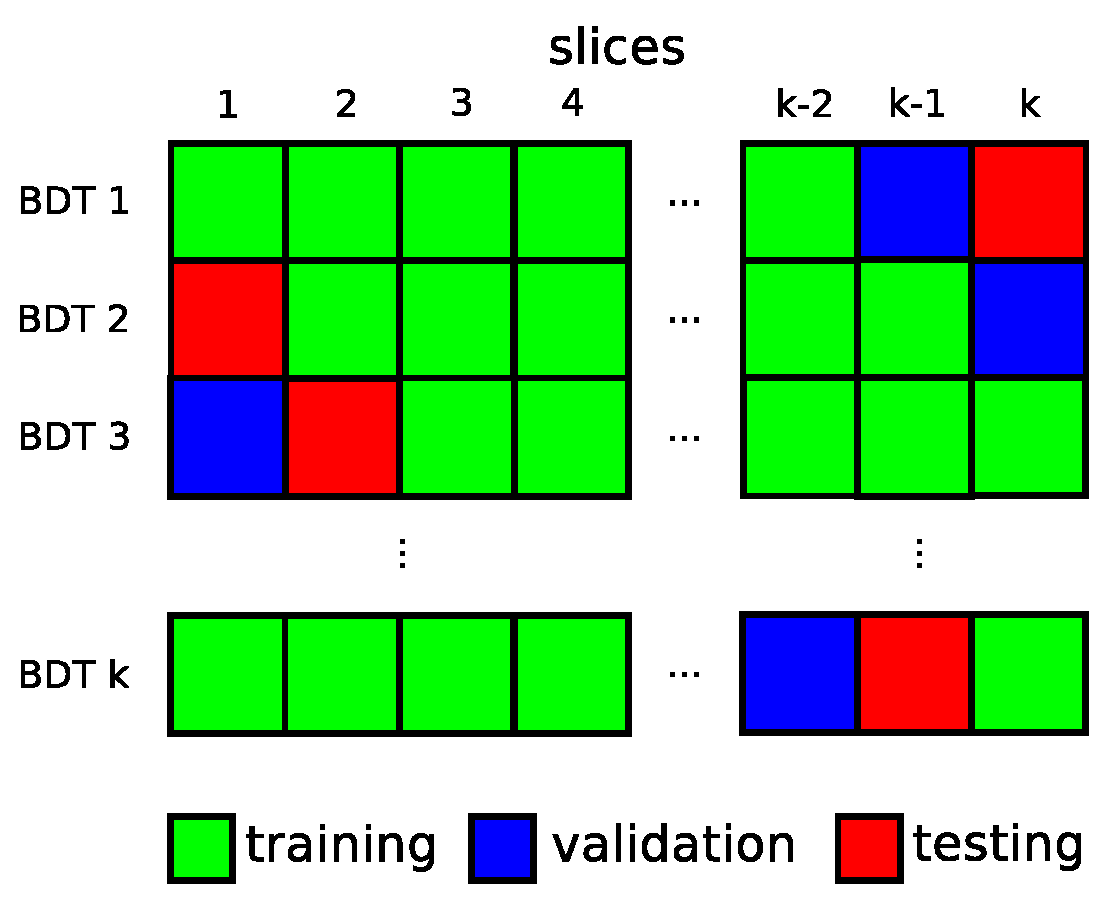
\includegraphics[width=0.6\textwidth]{./figures/mva/kfold-xval.eps}
    \caption{An illustration of the $k$-fold cross-validation scheme. The total set of simulated events is split into $k$ slices.
             All $k$ BDTs are trained, validated, and tested by using different combinations of the slices.}\label{fig:mva:kfold-xval}
\end{figure}

In the testing stage the $k$ BDTs need also be applied to data events.
The same approach as for simulated events could be used, where
a random number decides which BDT is used for which slice (random splitting).
However, some scientists do not like the idea that data are treated randomly.
Furthermore, random numbers cannot be reproduced on all computer systems, even if they are seeded.
In this case for each data event the output of every BDT could be calculated
and an average over all BDT outputs could be built (denoted as \emph{average}).
But this leads to another issue.
First, the simulated events and data events are treated in a different way.
Second, averaging over $k$ BDTs could lead to the effect, that events in border regions
are shifted towards the middle of the distribution, since the central limit theorem can be applied here.

In this analysis a third approach is used, the so-called \emph{modulo splitting}.
Every recorded data event in ATLAS is labeled with a unique number, the so-called event number.
This number is set once and not modified again.
The expression ``$\text{event number} \mod k$'' is used to split the data events into $k$ different slices.
This method was chosen because it treats data events similar to simulated events, but takes out the randomness of the splitting.
It needs to be checked that the data events are distributed equally in the different slices.
The distribution of ``$\text{event number} \mod k$'' is shown in \cref{fig:mva:event_number_mod} for all
data events which pass the MVA selection.
Within two standard deviations the count in each slice agrees with the average.
Therefore this splitting procedure does not introduce slices of unequal size.

\begin{figure}[htb]
    \centering
    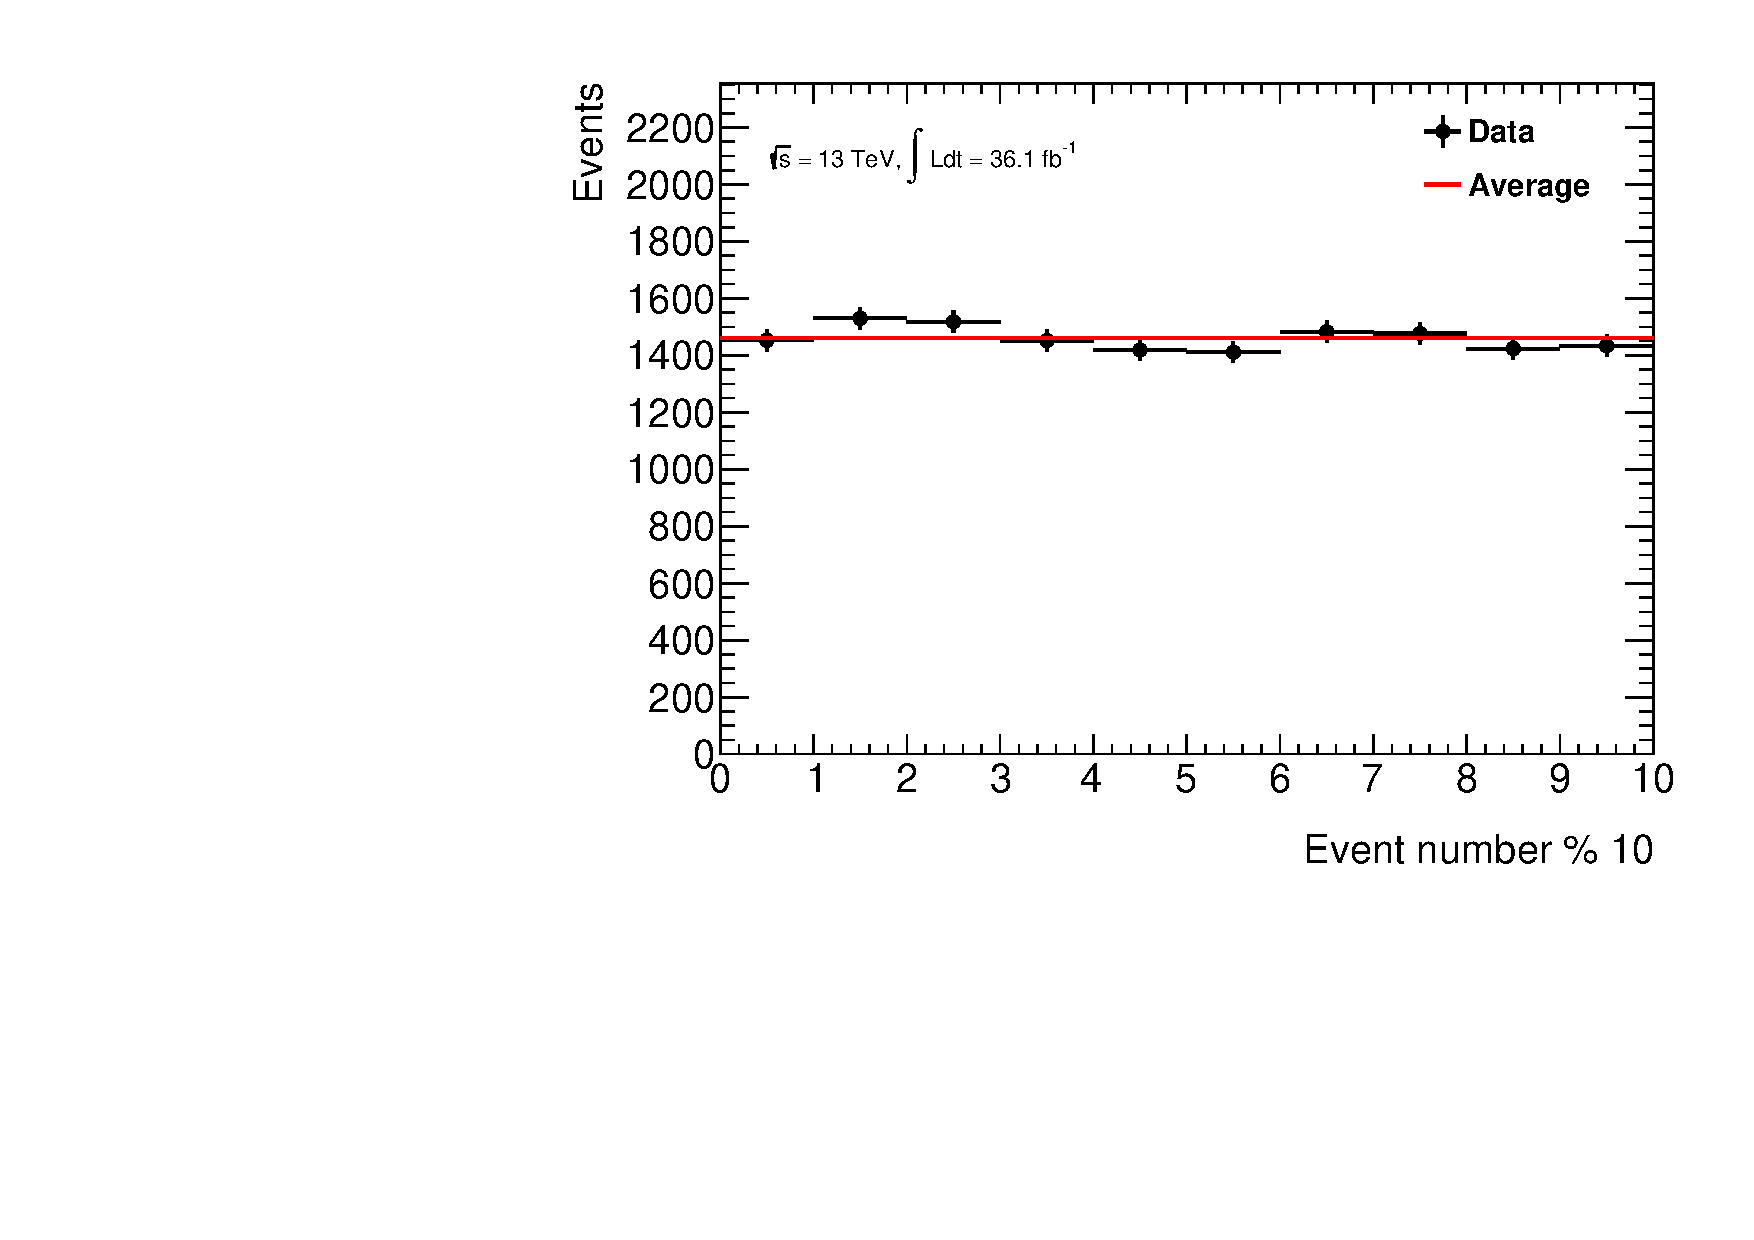
\includegraphics[width=0.7\textwidth]{./plots/mva/data_treatment/event_number_mod.pdf}
    \caption{Number of data events for each slice when splitting with ``$\text{event number} \mod k$'' is used.
             The plot shows data from the full 2015 and 2016 dataset which passed the MVA selection.}\label{fig:mva:event_number_mod}
\end{figure}

The three methods of data treatment are compared in \cref{fig:mva:data_treatment}.
Here the final BDTs which are selected in \cref{sec:mva:optimization} are used.
In the low-BDT-score regions in the boosted category the shift of events in the border region towards
the center when averaging over all BDTs can be seen.
Otherwise the methods agree within uncertainties.

\begin{figure}[htb]
    \centering
    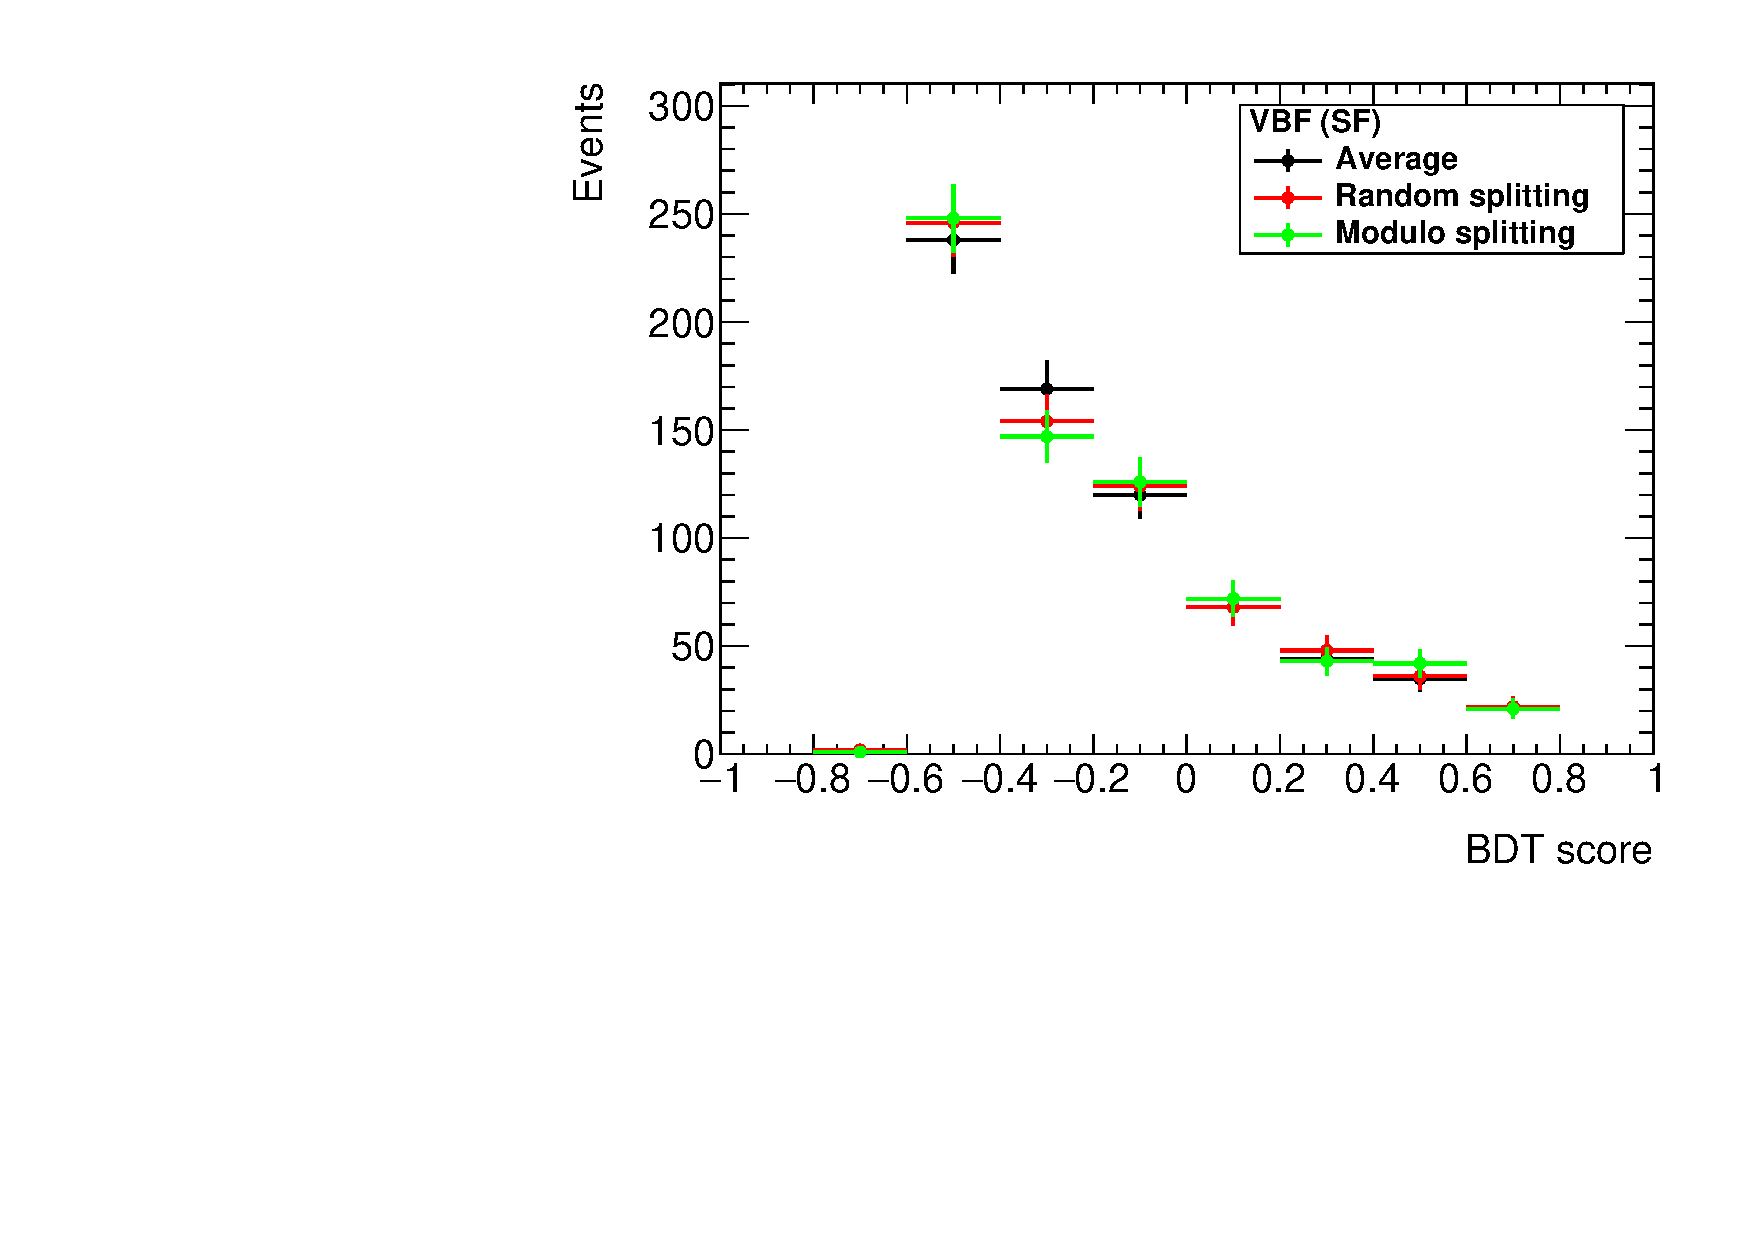
\includegraphics[width=0.45\textwidth]{./plots/mva/data_treatment/VBF_SF_average_vs_split.pdf}
    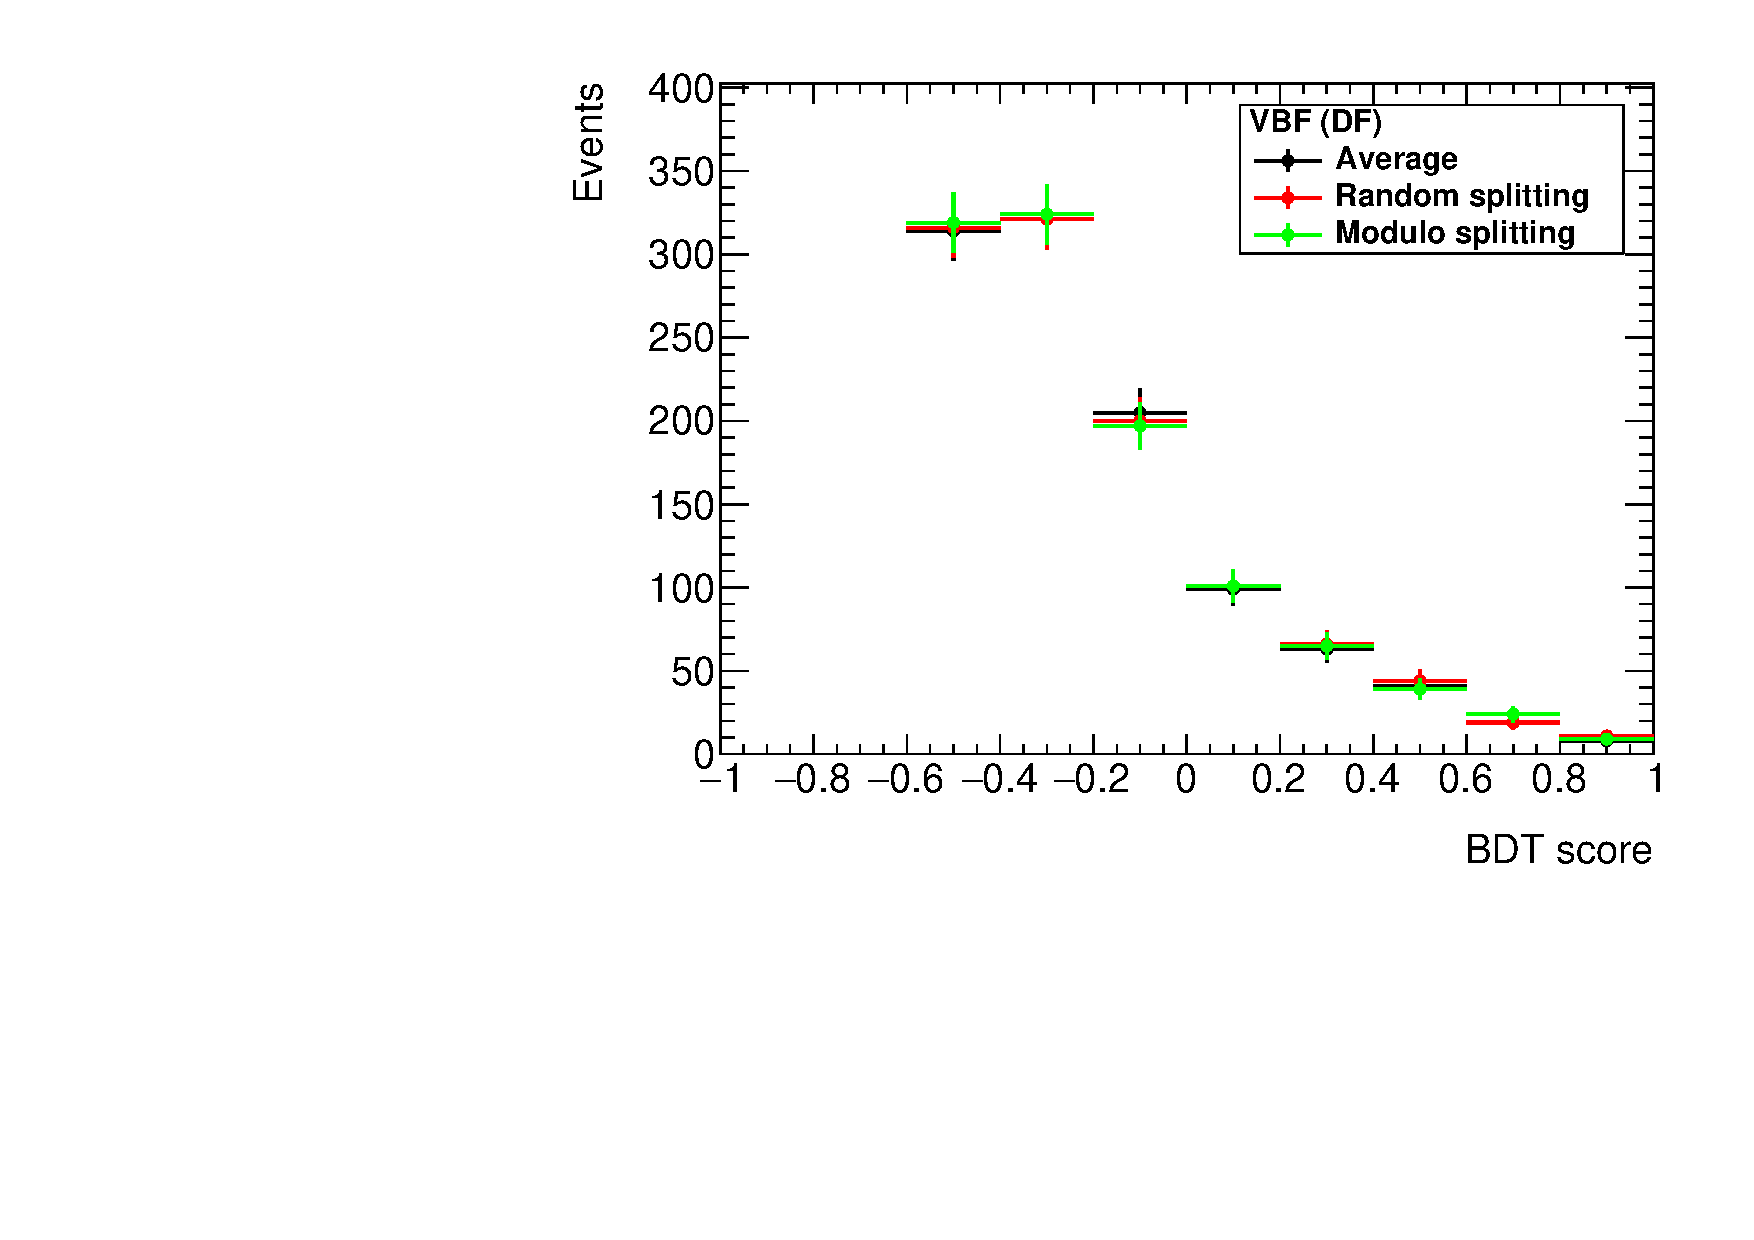
\includegraphics[width=0.45\textwidth]{./plots/mva/data_treatment/VBF_DF_average_vs_split.pdf} \\
    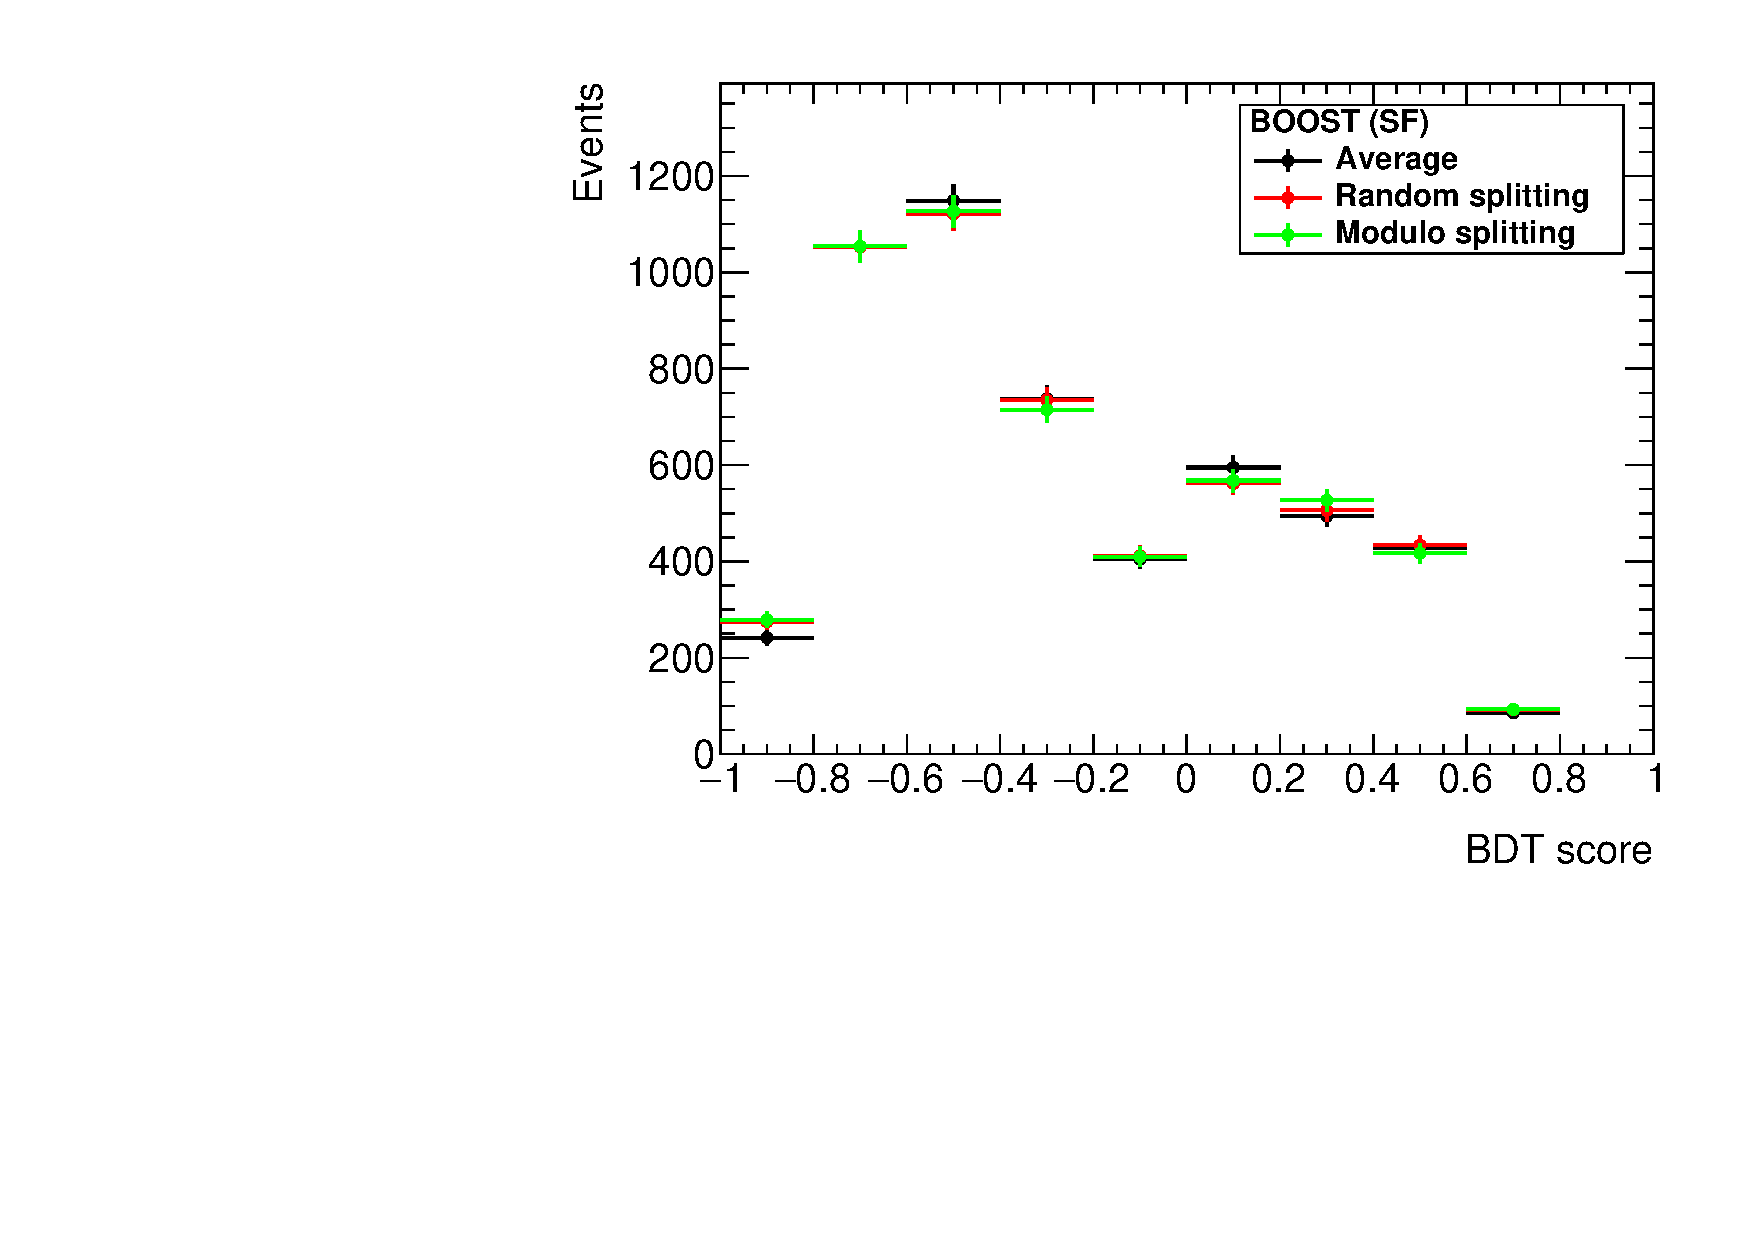
\includegraphics[width=0.45\textwidth]{./plots/mva/data_treatment/BOOST_SF_average_vs_split.pdf}
    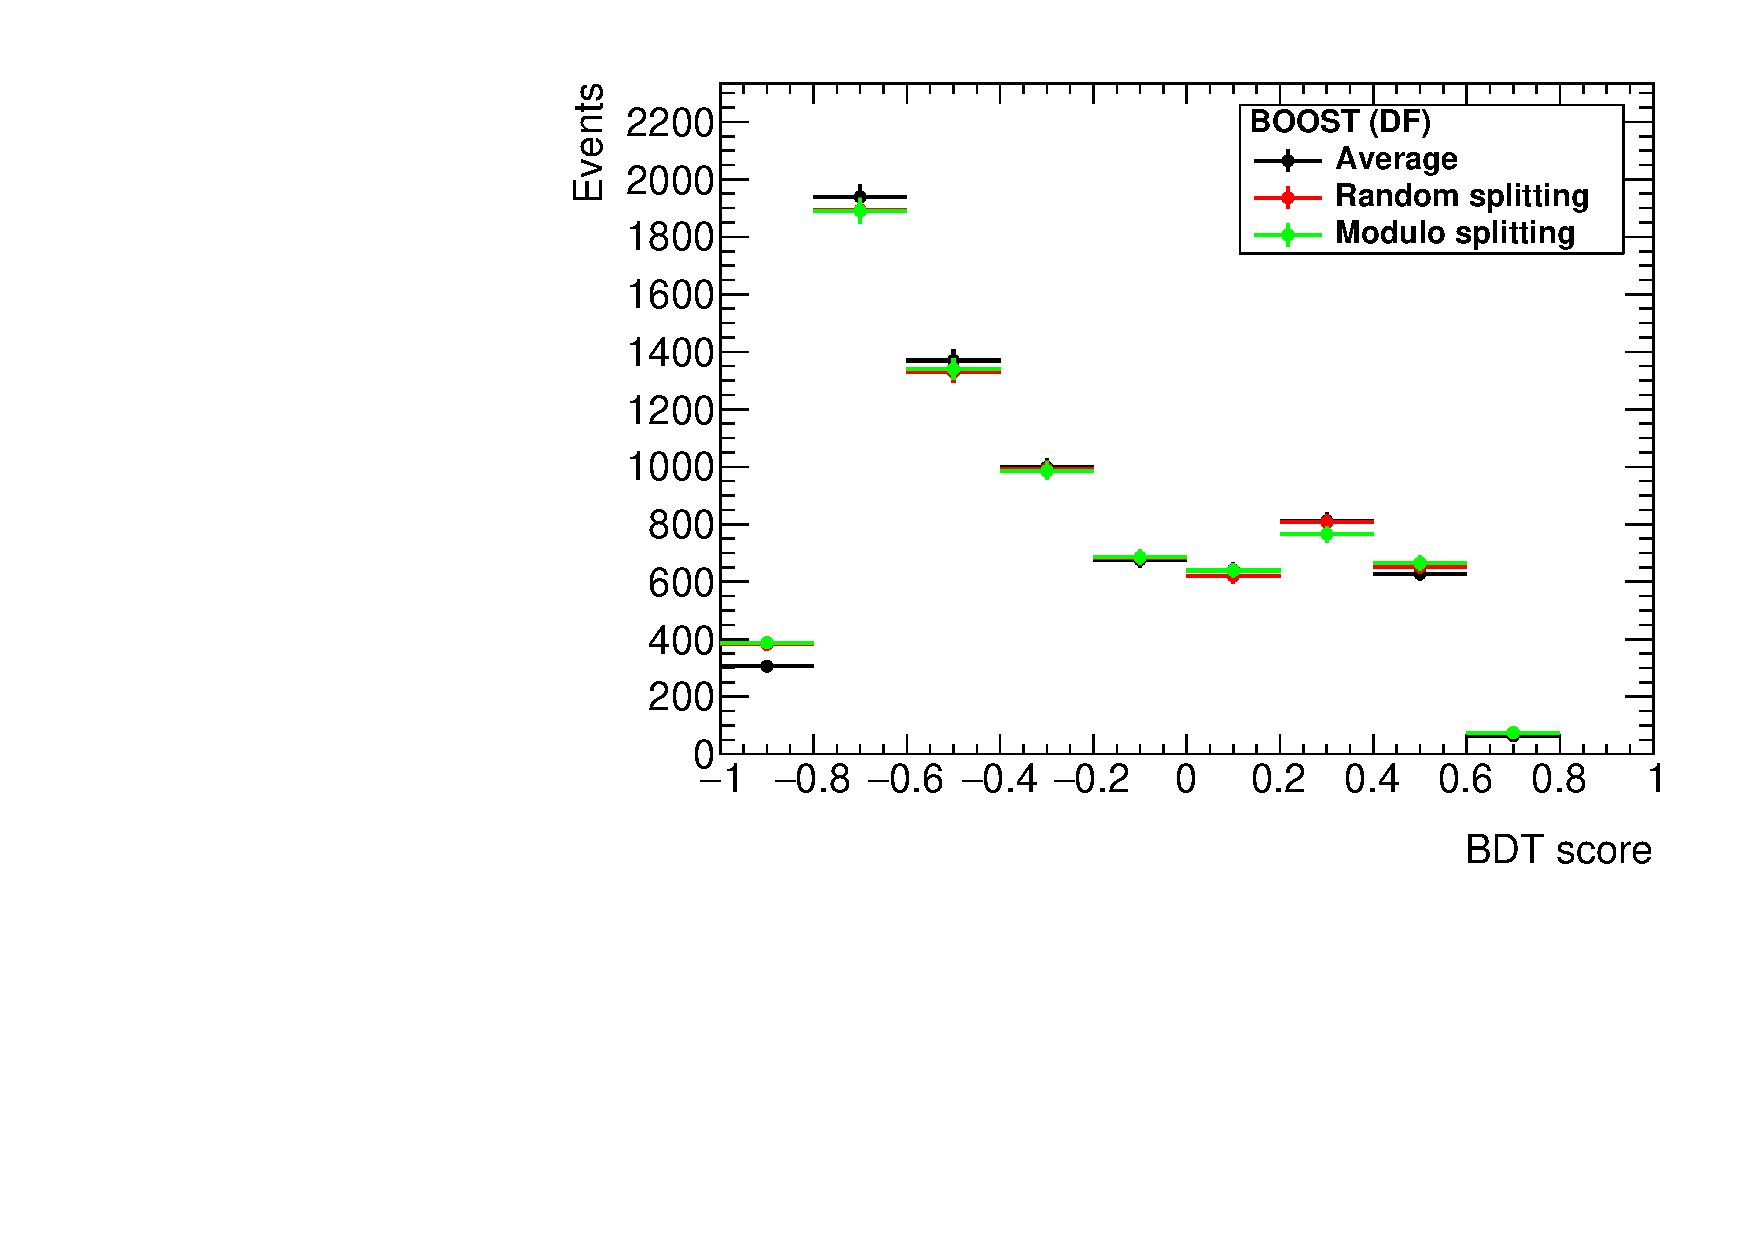
\includegraphics[width=0.45\textwidth]{./plots/mva/data_treatment/BOOST_DF_average_vs_split.pdf}
    \caption{Comparison of data treatment in $k$-fold cross-validation in the four MVA categories.
             The optimized BDTs from \cref{sec:mva:optimization} are used and are evaluated on the full
             2015 and 2016 dataset.}\label{fig:mva:data_treatment}
\end{figure}

\section{Optimization}\label{sec:mva:optimization}

The optimization is done individually in the four signal regions (VBF SF, VBF DF, boosted SF, boosted DF), which are defined in \cref{sec:mva:event_selection}.
In the VBF category only the VBF $\Htt$ sample is used for training and the boosted category uses only the ggF $\Htt$ sample as signal.
The other signal processes are discarded.
This decision was made even though the contributions of the VBF process in the boosted category and
the ggF process in the VBF category are not negligible.
Since the goal of this thesis is to measure the signal strength of $\Htt$ in the VBF- and ggF-production channel,
it makes sense to optimize the analysis for the measurement of the individual production modes.

The optimization procedure is divided into two steps.
First, the BDT hyperparameters are optimized. Here $54$ input variables are used. A full list of the considered observables can be found in \cref{app:mva:fulllistvars}.
However, such a high number of observables is not preferred, since the modelling of every observable needs to be tested.
Some observables are also highly correlated and provide only a tiny amount of new information.
Thus, the number of input variables for the BDTs is reduced in a second step, keeping only the variables which provide
the highest separation power.

\subsection{Figure of merit}\label{sub:mva:optimization:fom}

The separation power of a BDT can be assessed in different ways.
In this section several possible figures of merit are discussed,
which were considered for the estimation of the BDT performance.
These values are calculated on the validation set.

A common characteristic of a machine-learning model is the area under the receiver-operating characteristic (ROC) curve.
The ROC curve displays the rate of background rejection as a function of the rate of signal efficiency.
A larger area under the ROC curve indicates a better separation power.
The ROC curves are provided by TMVA\@.

Another figure of merit is the separation $\left<S^2\right>$, which is defined by~\cite{TMVA}
\begin{equation}
    \left<S^2\right> = \int_{-1}^1 \frac{{\left(\hat{y}_S(y) - \hat{y}_B(y)\right)}^2}{\hat{y}_S(y) + \hat{y}_B(y)} \dif y \,.
\end{equation}
The probability density functions of the output of the classifier are denoted as $\hat{y}_S$ and $\hat{y}_B$.
If the signal and background distribution have a complete overlap, the separation is zero.
Distributions with no overlap at all yield a separation of one.
The separation is also calculated by TMVA\@.

TMVA also provides a significance, which is calculated by
\begin{equation}
    Z_\text{TMVA} = \frac{\overline{y}_S - \overline{y}_B}{{\text{RMS}_S(y)}^2 + {\text{RMS}_B(y)}^2}
\end{equation}
Here $\overline{y}_{S}$ and $\overline{y}_{B}$ are the means of the classifier output for signal and background, respectively.
The root-mean-squares of the classifier output for signal and background are denoted as $\text{RMS}_S(y)$ and $\text{RMS}_B$.

Another way to calculate a significance is with the \emph{binned significance}.
For this histograms with $10$ equidistant bins of the BDT distribution for signal and background is used.
If a bin contains less than $10$ background events, it is merged with its left neighbor (the most left bin is merged
with its right neighbor).
In each bin the significance is calculated with the asymptotic formula~\cite{CowanAsymSig}
\begin{equation}
    Z_\text{asym}(s, b) = \sqrt{2 \left( (s+b) \ln \left(1 + \frac{s}{b} \right) - s \right)} \,,
\end{equation}
where $s$ and $b$ are the expected signal and background yields.
The binned significance $Z_\text{binned}$ is the quadratic sum of the significances in the individual bins,
\begin{equation}
    Z_\text{binned} = \sqrt{\sum_i {Z_\text{asym}(s_i, b_i)}^2} \,.
\end{equation}
This significance is a simple approximation of the significance of the complete fit model, which is discussed in \cref{cha:fit}.

Of course the significance of the fit model can also be used to estimate the performance of a BDT\@.
This figure-of-merit is actually used for the optimization, since it the closest approximation of the real fit.
This method is actually used for the optimization.
However, not the full fit model is applied.
Including all systematic variations (\cref{cha:systematics}) would need too much computing power to run the optimization in a reasonable timescale.
Therefore, the fit is done without the systematic variations, which is also denoted as \emph{stat.\ only fit} (``statistics only'').
The fit is performed with Asimov data, i.e.\ the simulated events are used instead of the measured data, to avoid biasing the optimization due to the observed data.

\subsection{Hyperparameters}\label{sub:mva:hyperparameters}

In the first optimization step different hyperparameters for the BDTs
are optimized.
The boosting algorithm, number of trees in the boosting, maximum depth of the tree, minimum number of events in the final nodes,
and the learning rate are varied in a grid scan.
The values which were considered for those parameters can be found in \cref{tab:mva:hpyerparameterscan}.
This leads to a total of 630 BDTs which need to be trained for each region.

\begin{table}[htpb]
    \centering
    \caption{Values of the BDT hyperparameters which are used in the first optimization step.
    The hyperparameters are explained in \cref{sec:bdt:hyperparameters}.}\label{tab:mva:hpyerparameterscan}
    \begin{tabular}{ll}
        \toprule
        Hyperparameter   & Values \\ \midrule
        BoostType   & AdaBoost, Grad (gradient boost) \\
        NTrees      & $50, 250, 500, 750, 1000$ \\
        MaxDepth    & $2, 3, 4, 5, 7, 10$ \\
        MinNodeSize & $\SI{1}{\percent}, \SI{5}{\percent}, \SI{10}{\percent}$ \\
        Shrinkage   & $0.05, 0.1, 0.2, 0.5$ \\
        AdaBoostBeta& $0.1, 0.5, 0.8$ \\
        \bottomrule
    \end{tabular}
\end{table}

\subsubsection{General observations}

Before the best BDT hyperparameters are chosen first a few general trends are discussed.
The significance of the stat.\ only Asimov fit depending on the boosting algorithm is shown in \cref{fig:mva:scan:boosttype}.
In all four regions the gradient-boosting algorithm yields on average a better significance than the AdaBoost algorithm.
For the VBF categories between 250 and 750 boosting iterations are preferred, in the boosted categories also BDTs with
1000 boosting iterations yield a comparable significance, as can be seen in \cref{fig:mva:scan:ntrees}.
In the VBF SF and boosted DF category a maximum depth of at least 4 yields the best significance, as shown
in \cref{fig:mva:scan:maxdepth}.
In the boosted DF category also BDTs with a maximum depth of 3 return a good significance.
A general dependence of the separation power of the BDTs on the minimum number of events in the final
nodes could not be observed (\cref{fig:mva:scan:minnodesize}).
A lower training rate results most of the time in a higher significance, as can be seen in \cref{fig:mva:scan:shrinkage,fig:mva:scan:adaboostbeta}.

\begin{figure}[htb]
    \centering
    \begin{subfigure}[t]{0.45\textwidth}
        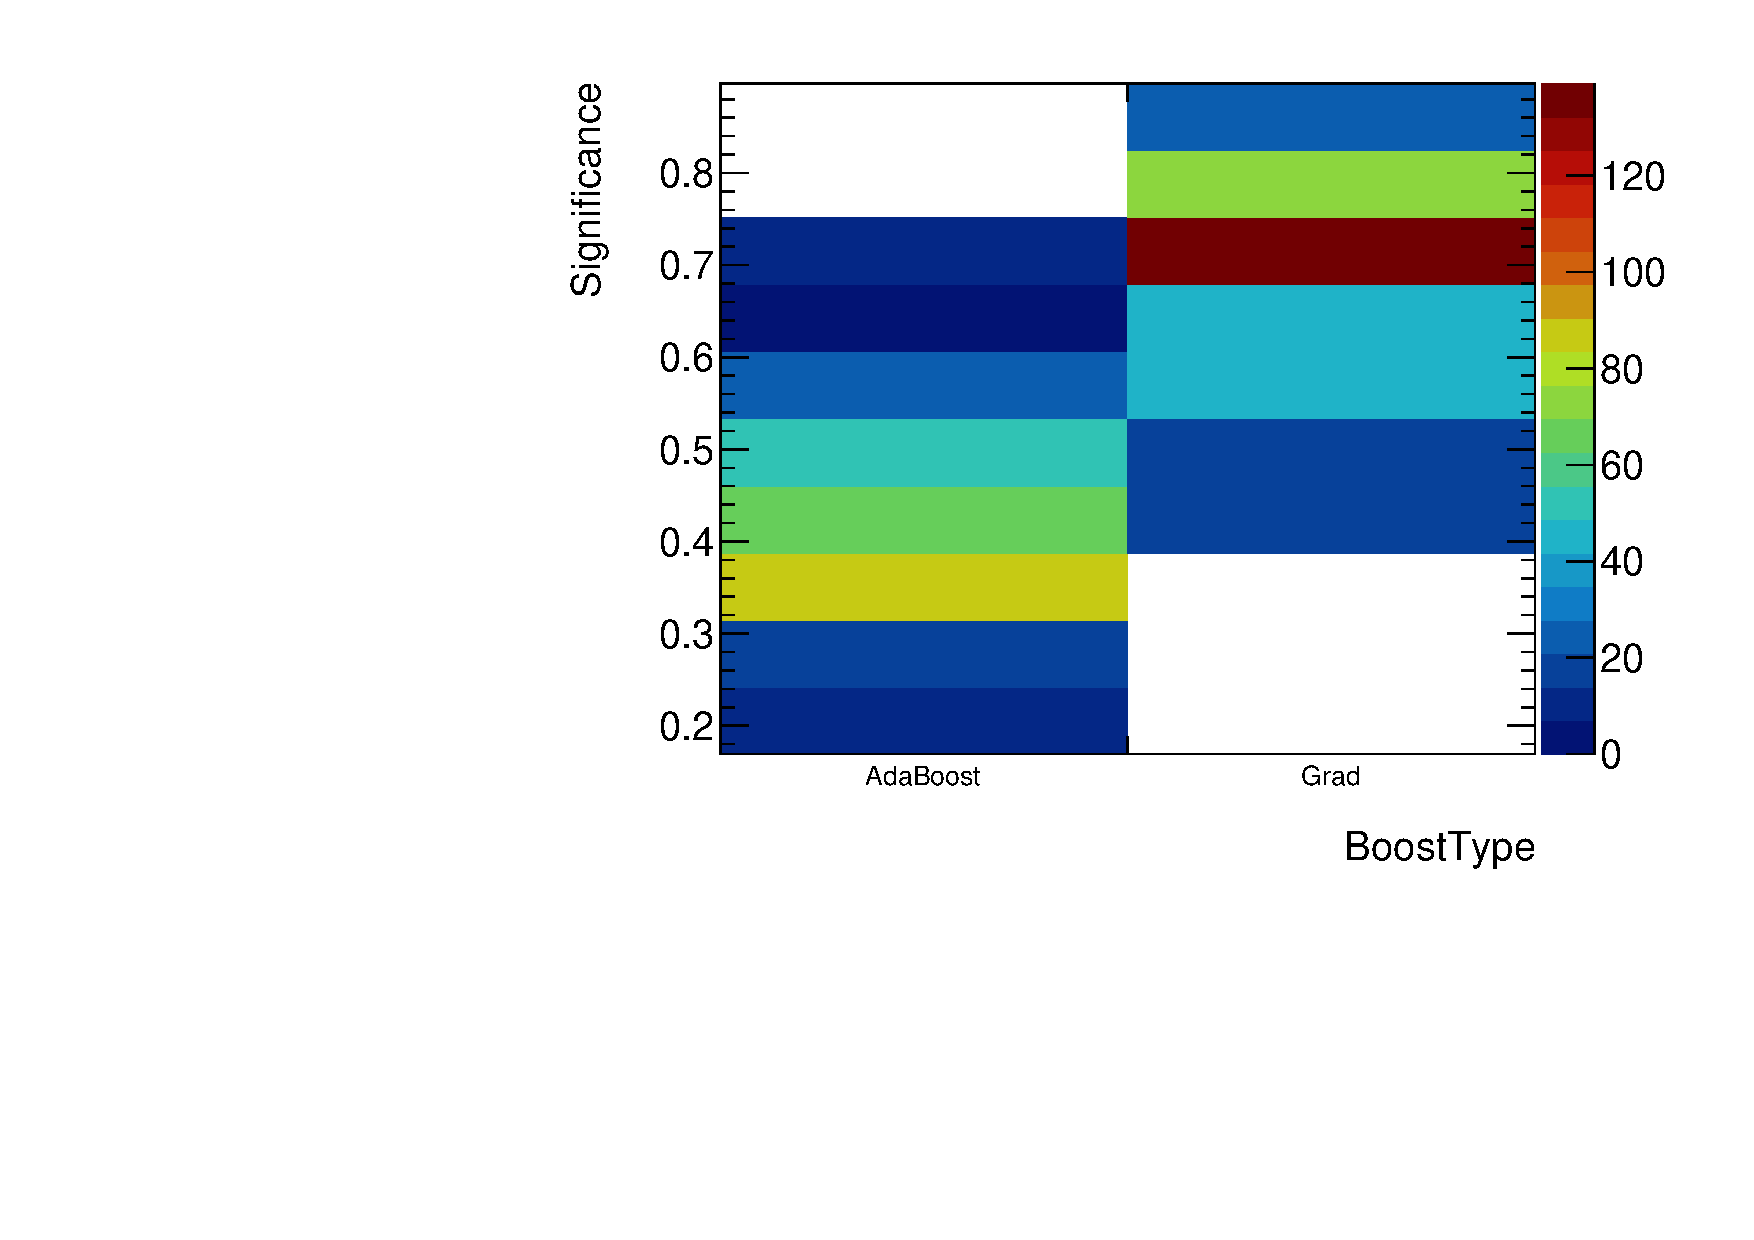
\includegraphics[width=\textwidth,page=1]{./plots/mva/scan/VBF_SF_setting_vs_binned_sig.pdf}
        \caption{VBF SF}
    \end{subfigure}
    \begin{subfigure}[t]{0.45\textwidth}
        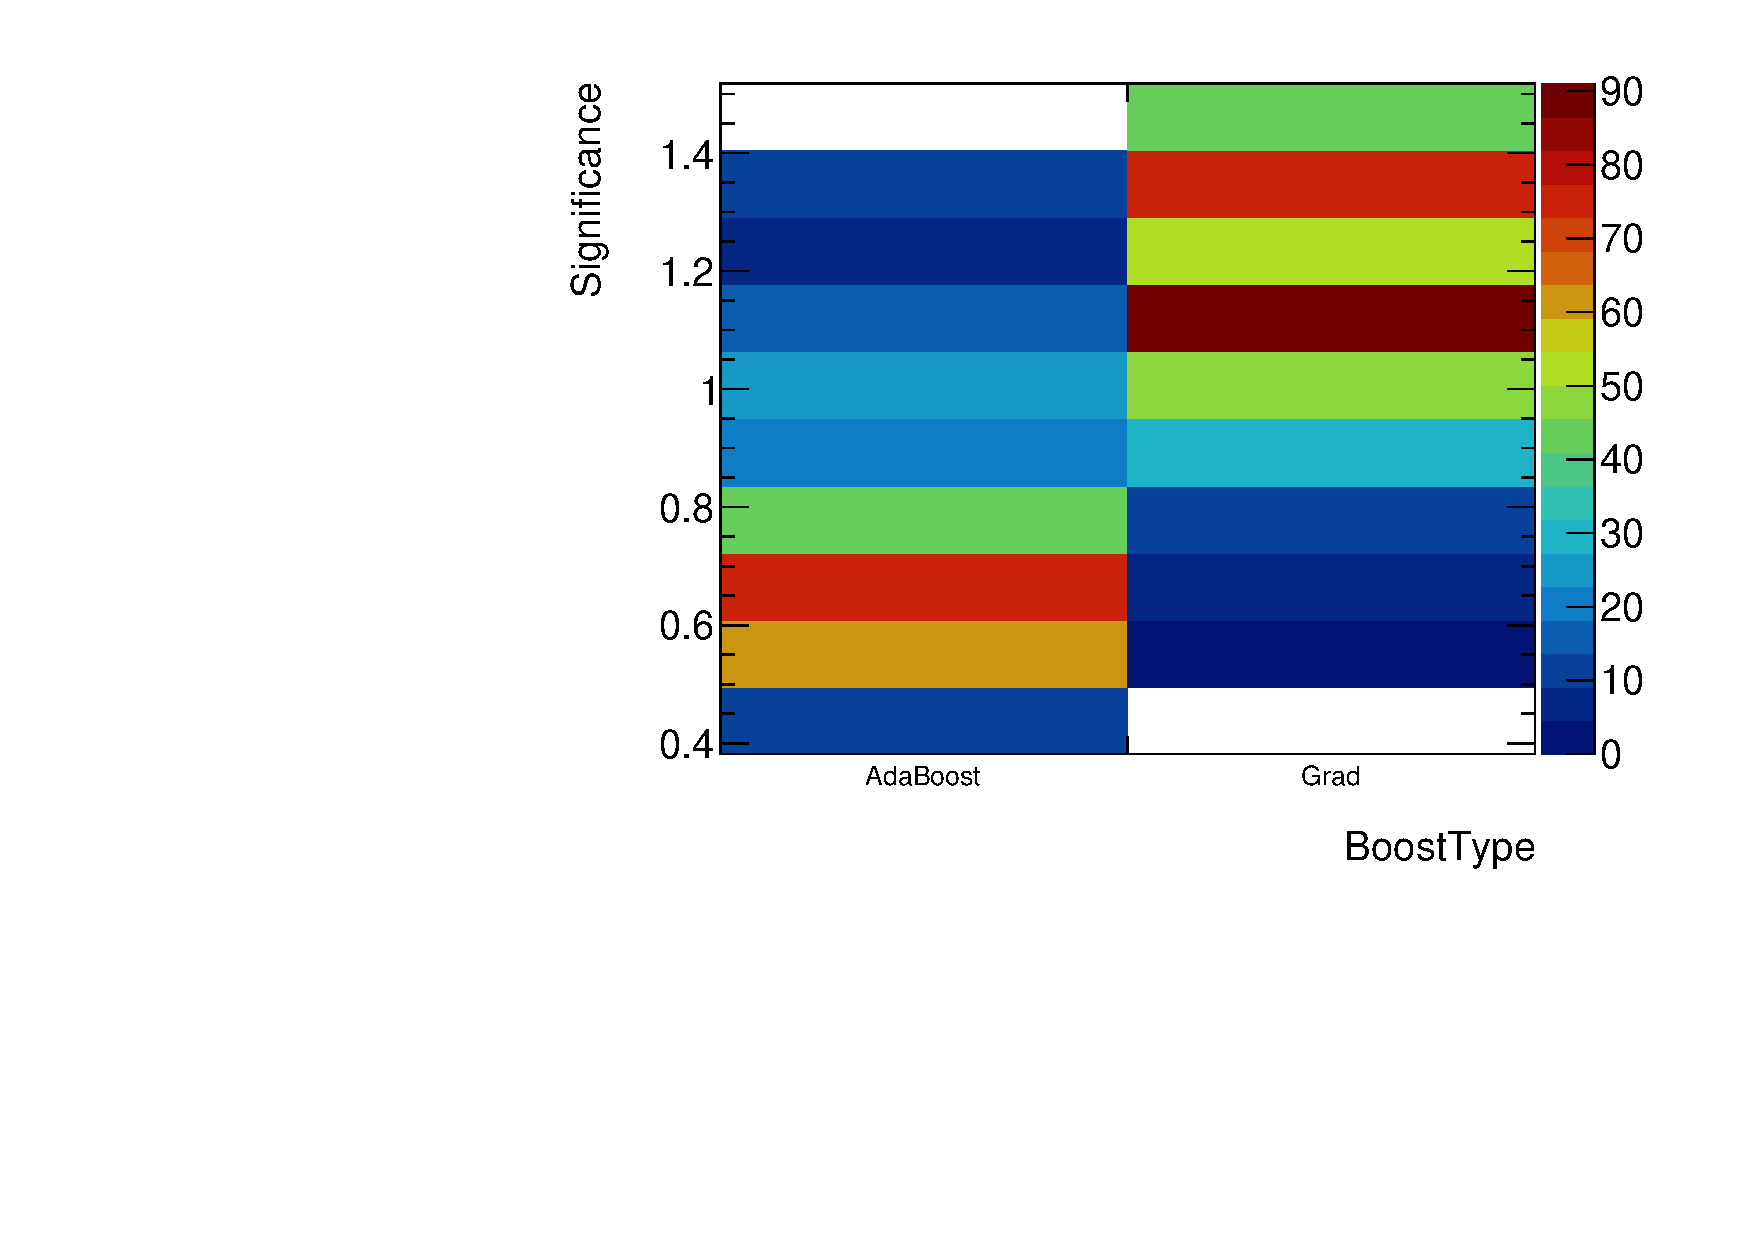
\includegraphics[width=\textwidth,page=1]{./plots/mva/scan/VBF_DF_setting_vs_binned_sig.pdf}
        \caption{VBF DF}
    \end{subfigure}
    \begin{subfigure}[t]{0.45\textwidth}
        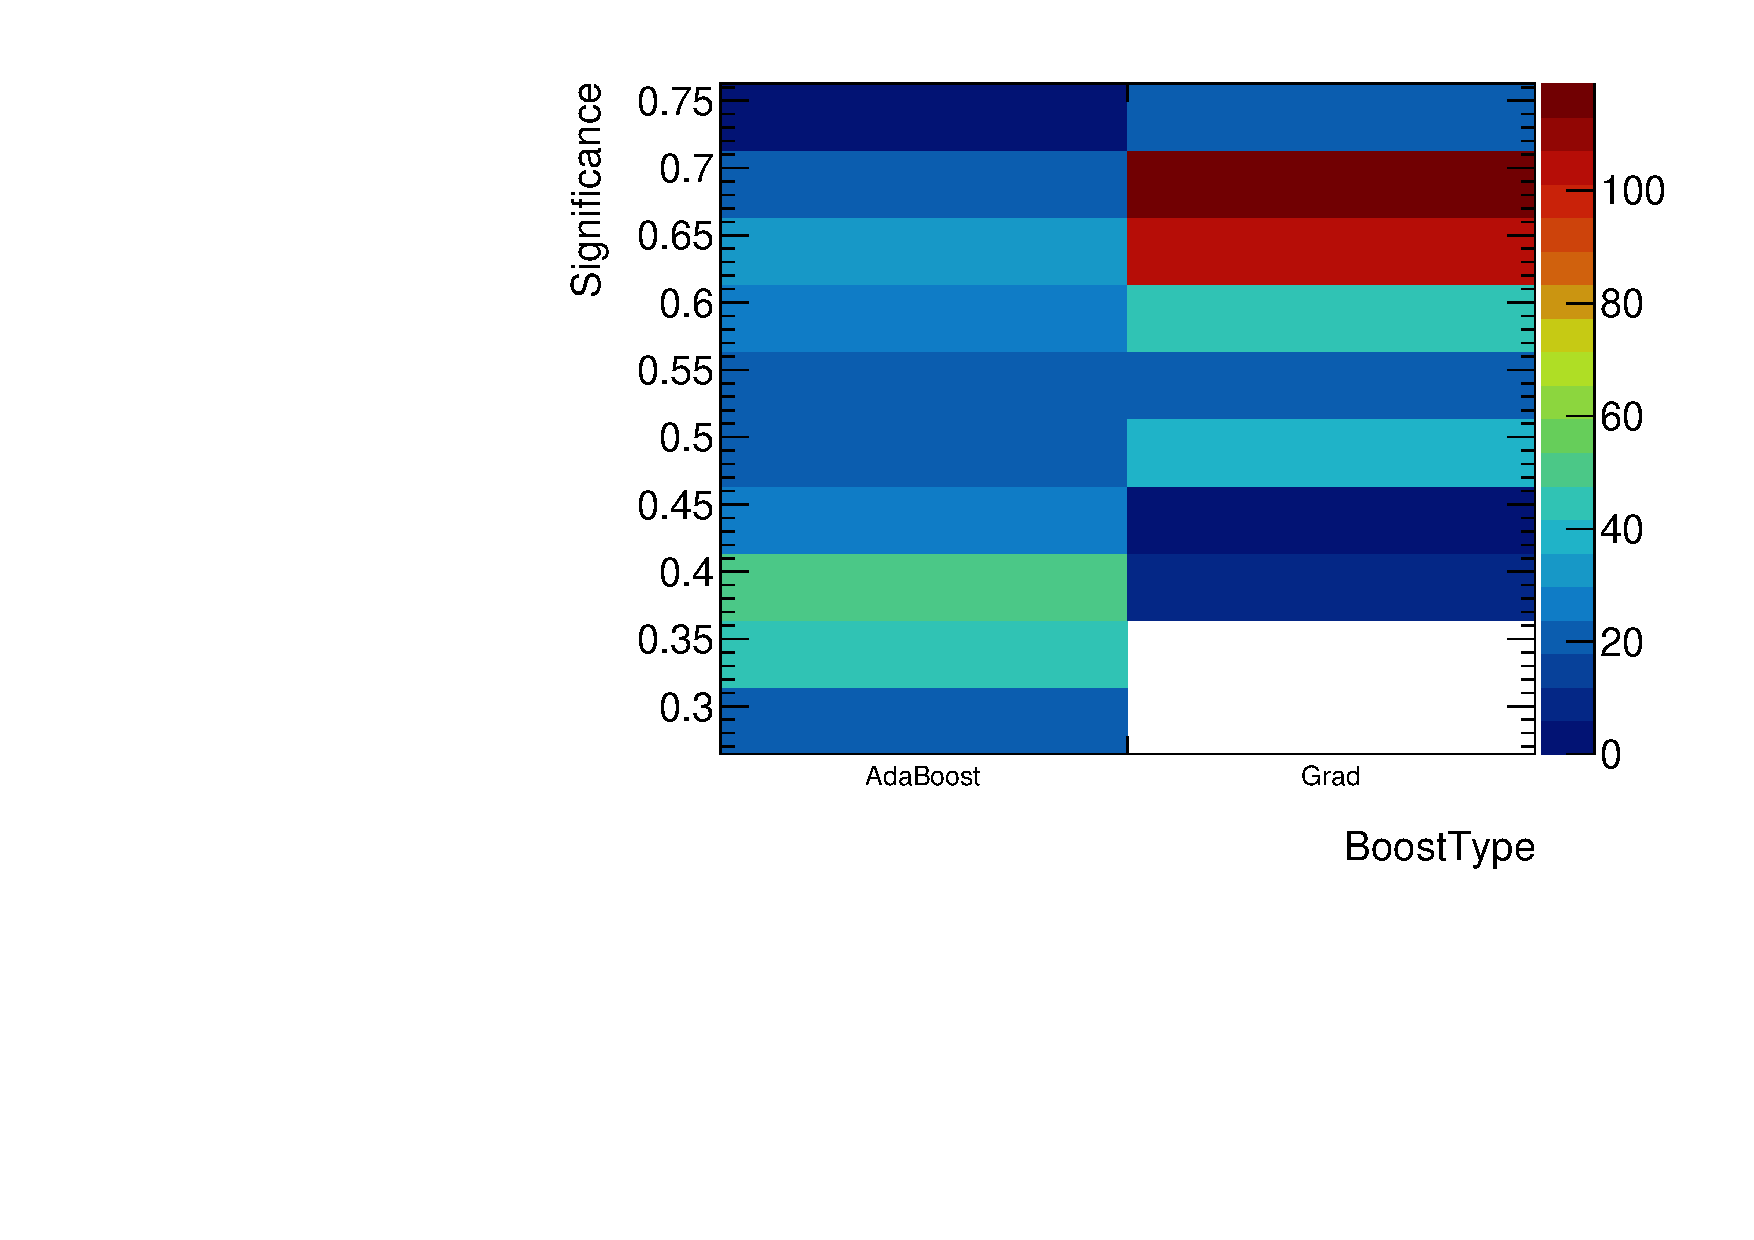
\includegraphics[width=\textwidth,page=1]{./plots/mva/scan/BOOST_SF_setting_vs_binned_sig.pdf}
        \caption{Boosted SF}
    \end{subfigure}
    \begin{subfigure}[t]{0.45\textwidth}
        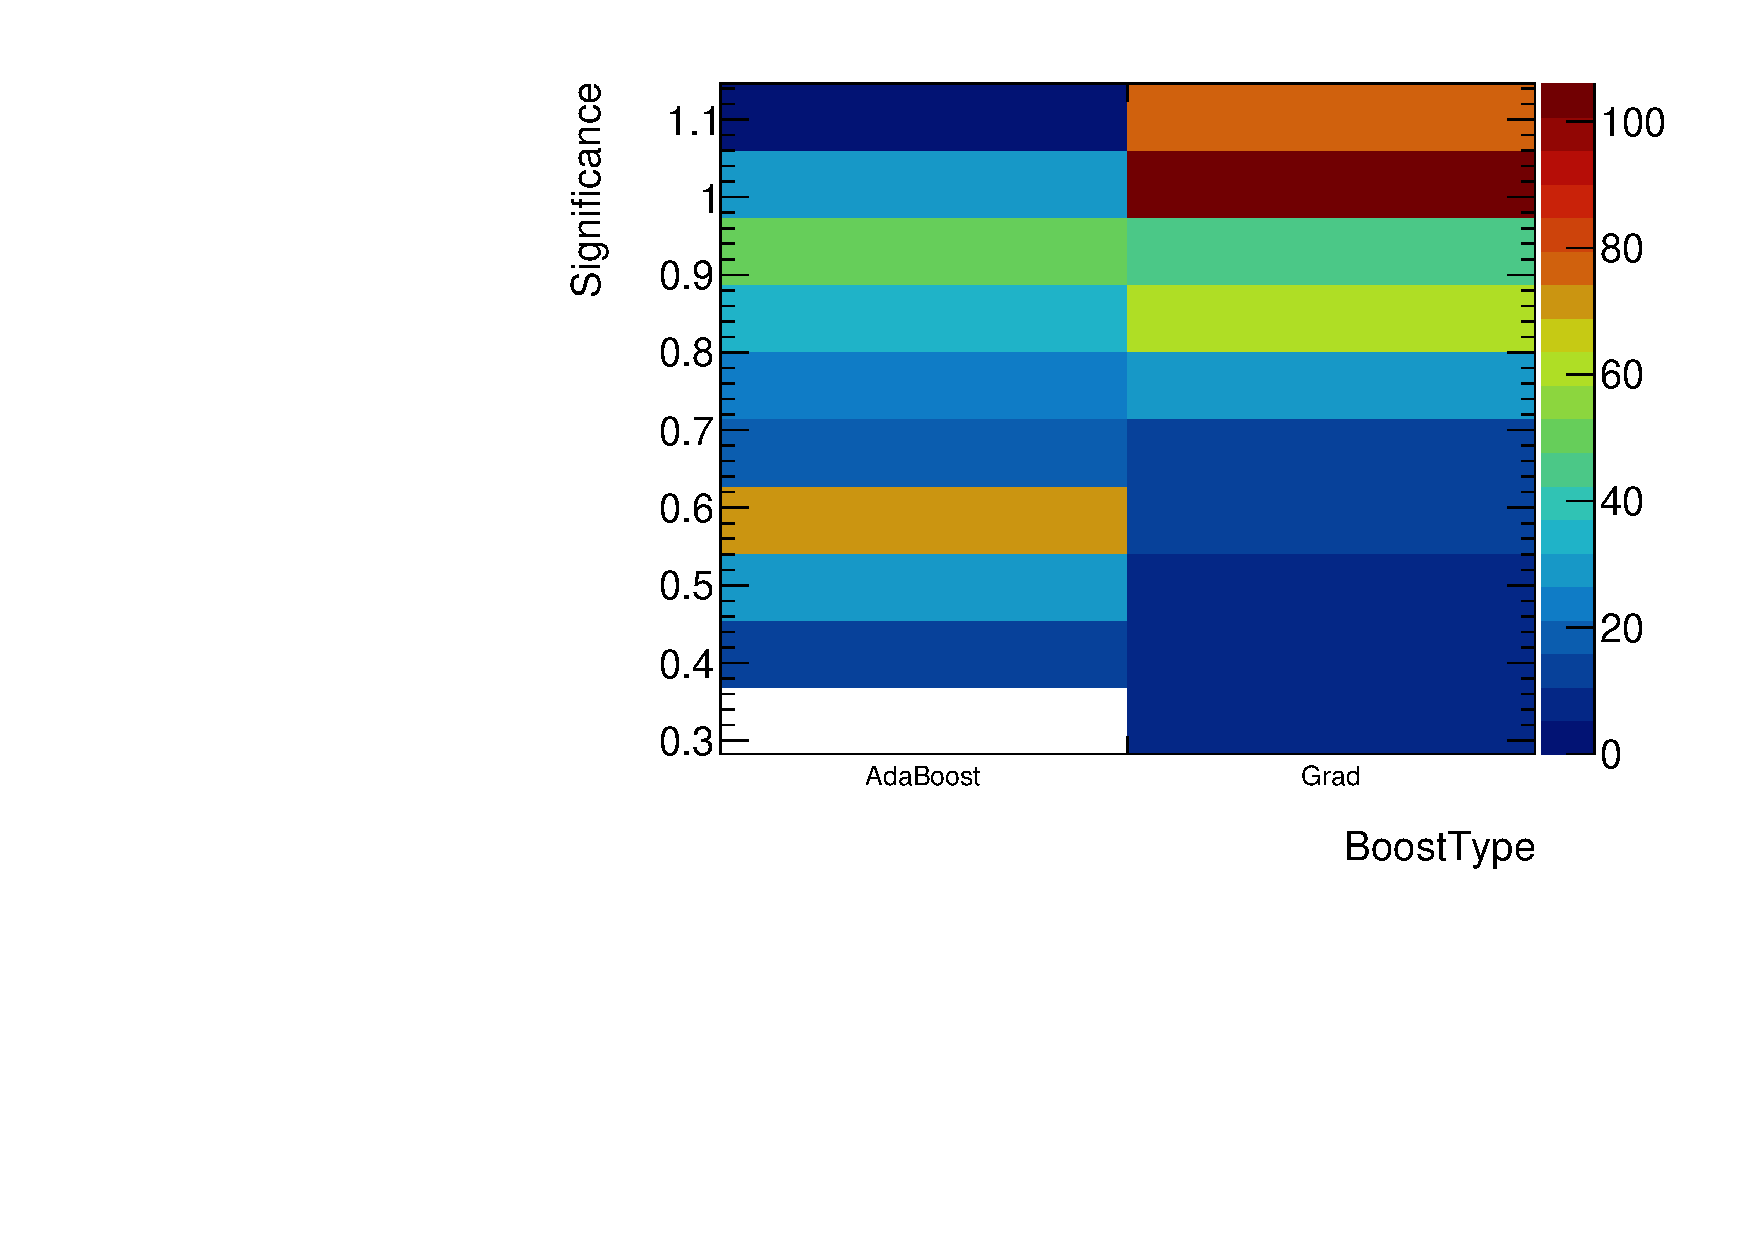
\includegraphics[width=\textwidth,page=1]{./plots/mva/scan/BOOST_DF_setting_vs_binned_sig.pdf}
        \caption{Boosted DF}
    \end{subfigure}
    \caption{Significance of all trained BDTs depending on the boosting algorithm for each region.}~\label{fig:mva:scan:boosttype}
\end{figure}

\begin{figure}[htb]
    \centering
    \begin{subfigure}[t]{0.45\textwidth}
        \includegraphics[width=\textwidth,page=2]{./plots/mva/scan/VBF_SF_setting_vs_binned_sig.pdf}
        \caption{VBF SF}
    \end{subfigure}
    \begin{subfigure}[t]{0.45\textwidth}
        \includegraphics[width=\textwidth,page=2]{./plots/mva/scan/VBF_DF_setting_vs_binned_sig.pdf}
        \caption{VBF DF}
    \end{subfigure}
    \begin{subfigure}[t]{0.45\textwidth}
        \includegraphics[width=\textwidth,page=2]{./plots/mva/scan/BOOST_SF_setting_vs_binned_sig.pdf}
        \caption{Boosted SF}
    \end{subfigure}
    \begin{subfigure}[t]{0.45\textwidth}
        \includegraphics[width=\textwidth,page=2]{./plots/mva/scan/BOOST_DF_setting_vs_binned_sig.pdf}
        \caption{Boosted DF}
    \end{subfigure}
    \caption{Significance of all trained BDTs depending on the number of trees used in boosting for each region.}~\label{fig:mva:scan:ntrees}
\end{figure}

\begin{figure}[htb]
    \centering
    \begin{subfigure}[t]{0.45\textwidth}
        \includegraphics[width=\textwidth,page=3]{./plots/mva/scan/VBF_SF_setting_vs_binned_sig.pdf}
        \caption{VBF SF}
    \end{subfigure}
    \begin{subfigure}[t]{0.45\textwidth}
        \includegraphics[width=\textwidth,page=3]{./plots/mva/scan/VBF_DF_setting_vs_binned_sig.pdf}
        \caption{VBF DF}
    \end{subfigure}
    \begin{subfigure}[t]{0.45\textwidth}
        \includegraphics[width=\textwidth,page=3]{./plots/mva/scan/BOOST_SF_setting_vs_binned_sig.pdf}
        \caption{Boosted SF}
    \end{subfigure}
    \begin{subfigure}[t]{0.45\textwidth}
        \includegraphics[width=\textwidth,page=3]{./plots/mva/scan/BOOST_DF_setting_vs_binned_sig.pdf}
        \caption{Boosted DF}
    \end{subfigure}
    \caption{Significance of all trained BDTs depending on the maximum depth of the decision trees for each region.}~\label{fig:mva:scan:maxdepth}
\end{figure}

\begin{figure}[htb]
    \centering
    \begin{subfigure}[t]{0.45\textwidth}
        \includegraphics[width=\textwidth,page=4]{./plots/mva/scan/VBF_SF_setting_vs_binned_sig.pdf}
        \caption{VBF SF}
    \end{subfigure}
    \begin{subfigure}[t]{0.45\textwidth}
        \includegraphics[width=\textwidth,page=4]{./plots/mva/scan/VBF_DF_setting_vs_binned_sig.pdf}
        \caption{VBF DF}
    \end{subfigure}
    \begin{subfigure}[t]{0.45\textwidth}
        \includegraphics[width=\textwidth,page=4]{./plots/mva/scan/BOOST_SF_setting_vs_binned_sig.pdf}
        \caption{Boosted SF}
    \end{subfigure}
    \begin{subfigure}[t]{0.45\textwidth}
        \includegraphics[width=\textwidth,page=4]{./plots/mva/scan/BOOST_DF_setting_vs_binned_sig.pdf}
        \caption{Boosted DF}
    \end{subfigure}
    \caption{Significance of all trained BDTs depending on the minimum number events given as the fraction of all events for each region.}~\label{fig:mva:scan:minnodesize}
\end{figure}

\begin{figure}[htb]
    \centering
    \begin{subfigure}[t]{0.45\textwidth}
        \includegraphics[width=\textwidth,page=5]{./plots/mva/scan/VBF_SF_setting_vs_binned_sig.pdf}
        \caption{VBF SF}
    \end{subfigure}
    \begin{subfigure}[t]{0.45\textwidth}
        \includegraphics[width=\textwidth,page=5]{./plots/mva/scan/VBF_DF_setting_vs_binned_sig.pdf}
        \caption{VBF DF}
    \end{subfigure}
    \begin{subfigure}[t]{0.45\textwidth}
        \includegraphics[width=\textwidth,page=5]{./plots/mva/scan/BOOST_SF_setting_vs_binned_sig.pdf}
        \caption{Boosted SF}
    \end{subfigure}
    \begin{subfigure}[t]{0.45\textwidth}
        \includegraphics[width=\textwidth,page=5]{./plots/mva/scan/BOOST_DF_setting_vs_binned_sig.pdf}
        \caption{Boosted DF}
    \end{subfigure}
    \caption{Significance of all trained BDTs where the gradient boost algorithm was used depending on the learning rate for each region.}~\label{fig:mva:scan:shrinkage}
\end{figure}

\begin{figure}[htb]
    \centering
    \begin{subfigure}[t]{0.45\textwidth}
        \includegraphics[width=\textwidth,page=6]{./plots/mva/scan/VBF_SF_setting_vs_binned_sig.pdf}
        \caption{VBF SF}
    \end{subfigure}
    \begin{subfigure}[t]{0.45\textwidth}
        \includegraphics[width=\textwidth,page=6]{./plots/mva/scan/VBF_DF_setting_vs_binned_sig.pdf}
        \caption{VBF DF}
    \end{subfigure}
    \begin{subfigure}[t]{0.45\textwidth}
        \includegraphics[width=\textwidth,page=6]{./plots/mva/scan/BOOST_SF_setting_vs_binned_sig.pdf}
        \caption{Boosted SF}
    \end{subfigure}
    \begin{subfigure}[t]{0.45\textwidth}
        \includegraphics[width=\textwidth,page=6]{./plots/mva/scan/BOOST_DF_setting_vs_binned_sig.pdf}
        \caption{Boosted DF}
    \end{subfigure}
    \caption{Significance of all trained BDTs where the AdaBoost algorithm was used depending on the learning rate for each region.}~\label{fig:mva:scan:adaboostbeta}
\end{figure}

\FloatBarrier{}

\subsubsection{Result of optimization}

The overtraining of a BDT can be estimated by using the \emph{Kolmogorov--Smirnov test}~\cite{KSk, KSs} (KS-test).
Here the BDT output of training and validation set is compared for both the signal and background distribution.
The KS-test yields a probability between zero and one, where one indicates perfect agreement and zero no agreement at all.
Only BDTs which yield a KS-test probability for both signal and background distribution above $0.4$ are considered.
The exact choice of this threshold plays only a very minor role, since most BDTs have a KS-test probability of either one or zero,
as can be seen in \cref{fig:mva:scan:kstest}.

\begin{figure}[htb]
    \centering
    \begin{subfigure}[t]{0.45\textwidth}
        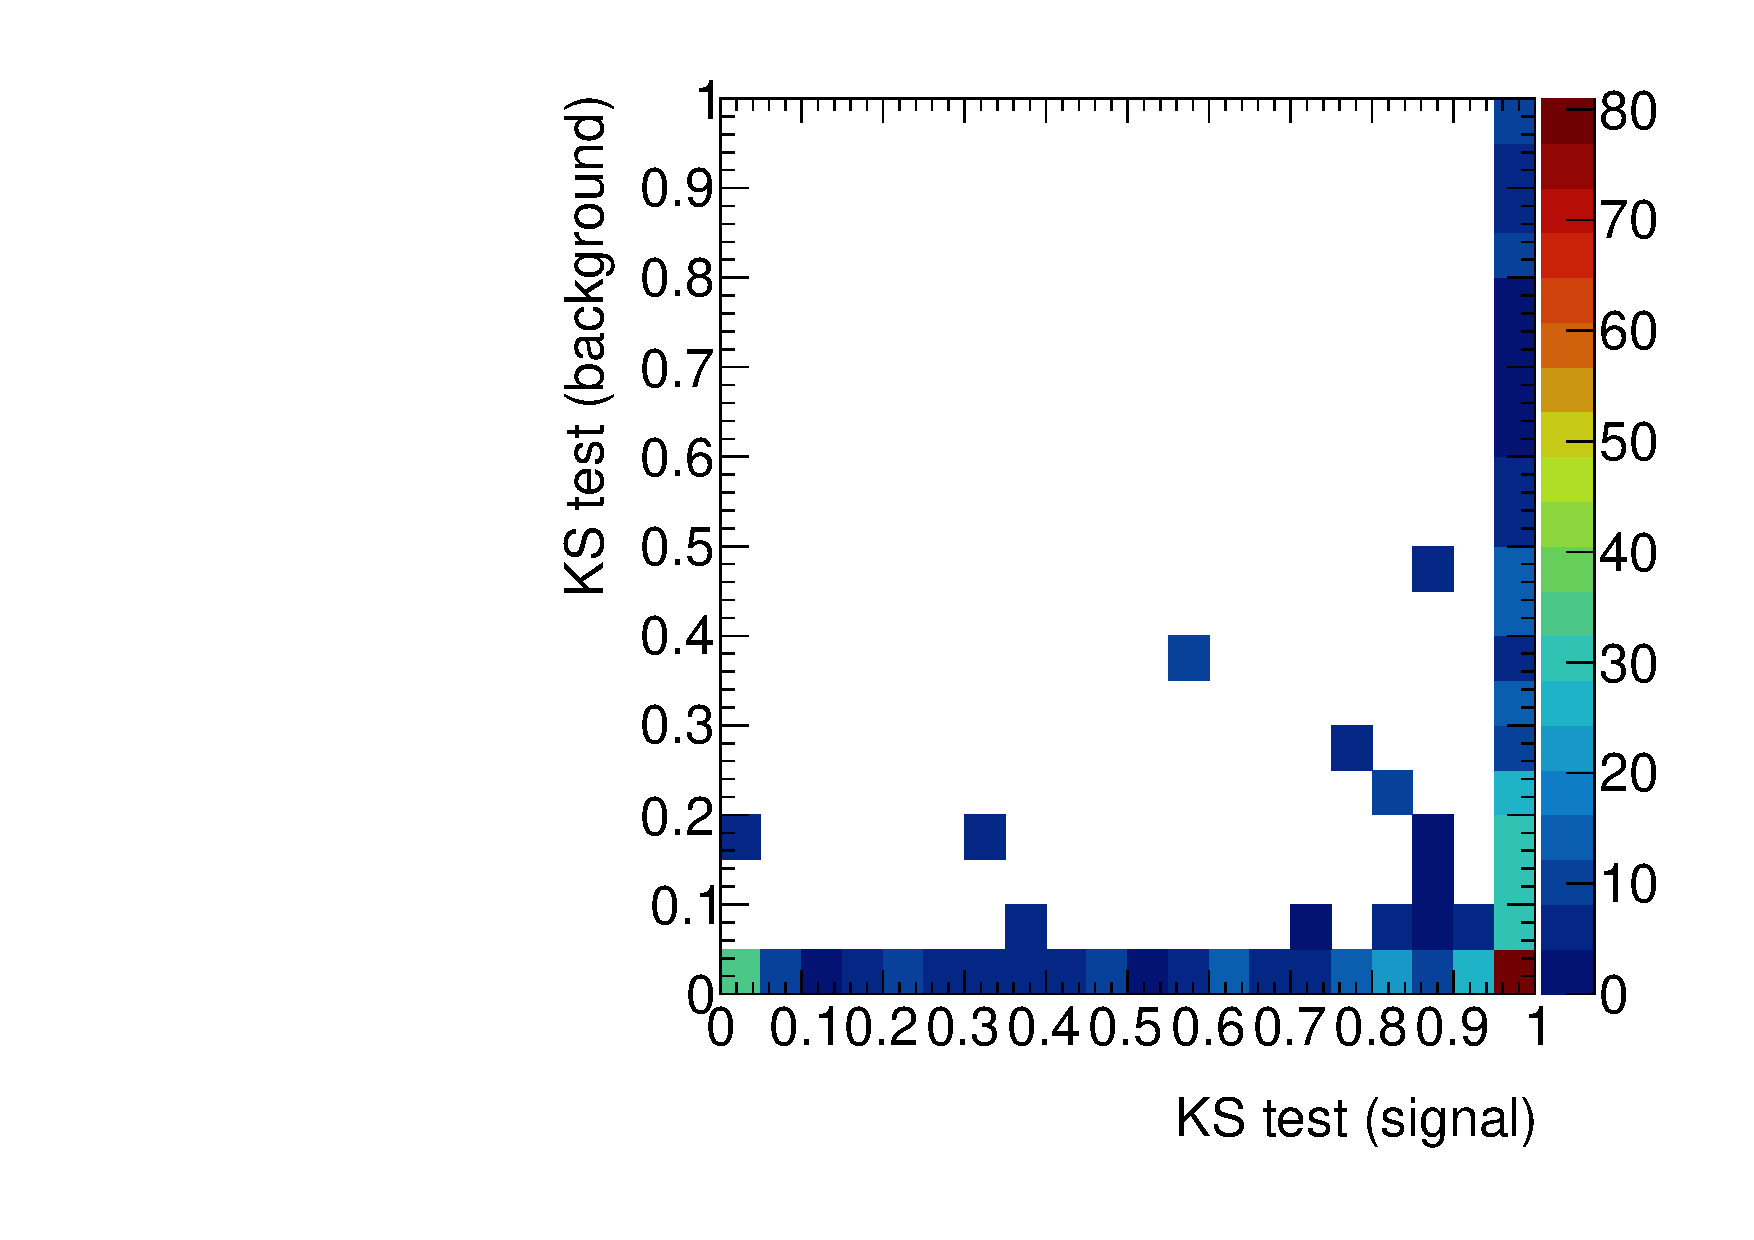
\includegraphics[width=\textwidth]{./plots/mva/scan/VBF_SF_ks_test_sig_vs_bkg.pdf}
        \caption{VBF SF}
    \end{subfigure}
    \begin{subfigure}[t]{0.45\textwidth}
        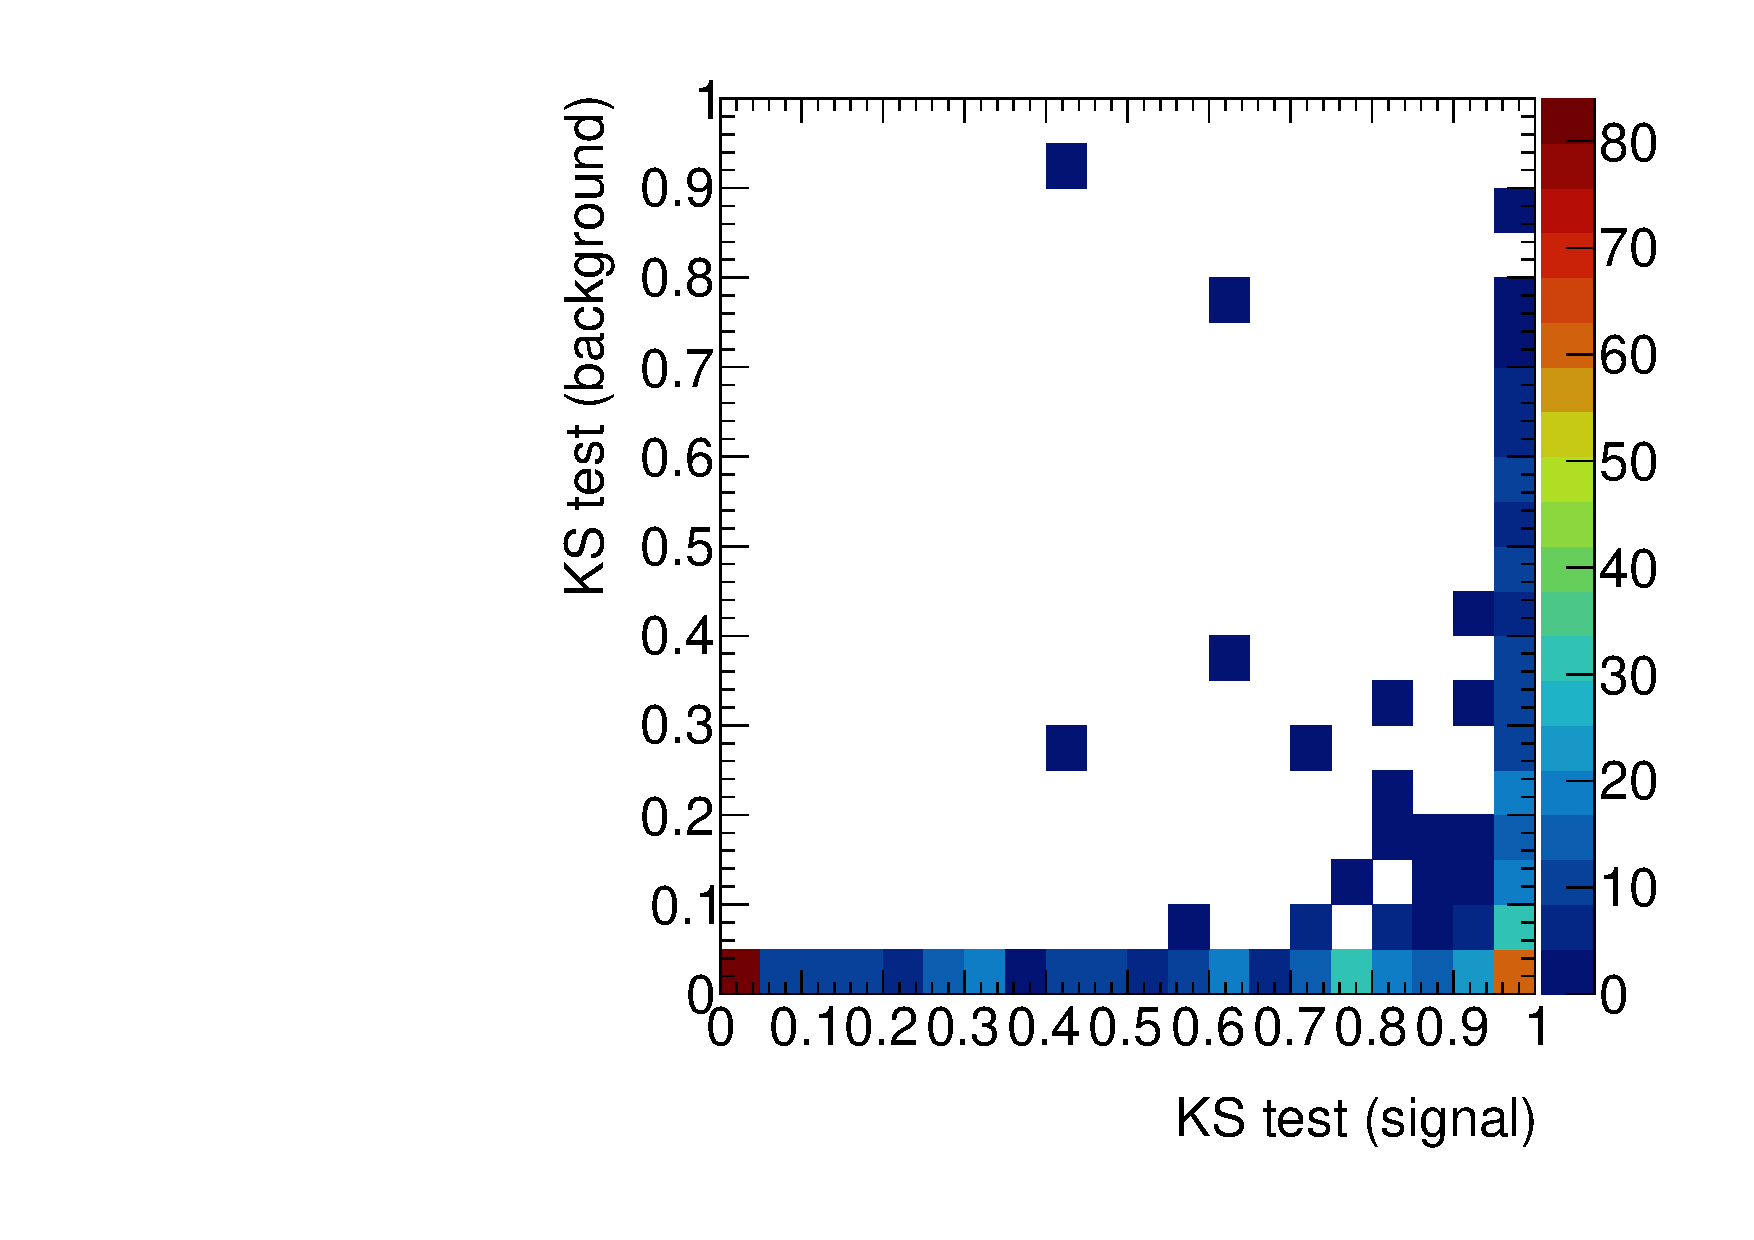
\includegraphics[width=\textwidth]{./plots/mva/scan/VBF_DF_ks_test_sig_vs_bkg.pdf}
        \caption{VBF DF}
    \end{subfigure}
    \begin{subfigure}[t]{0.45\textwidth}
        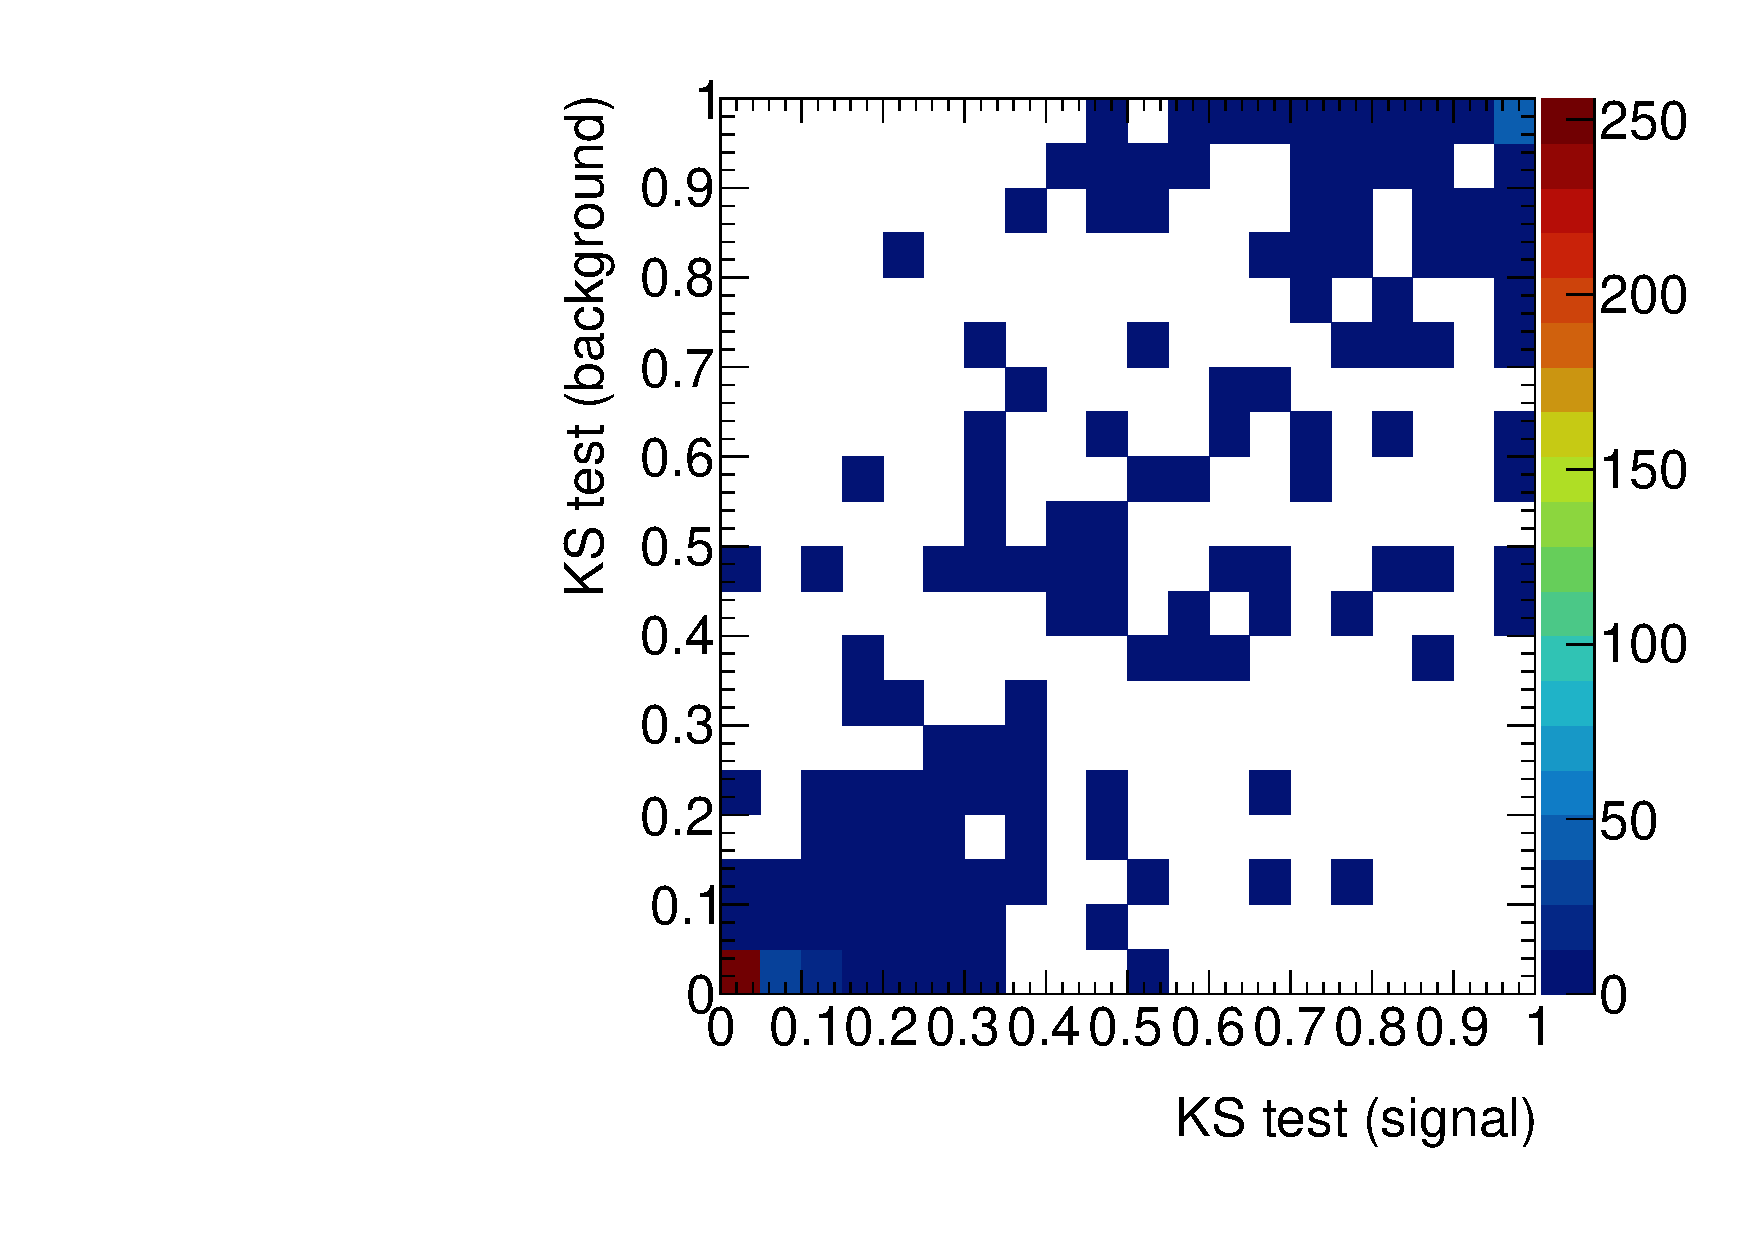
\includegraphics[width=\textwidth]{./plots/mva/scan/BOOST_SF_ks_test_sig_vs_bkg.pdf}
        \caption{Boosted SF}
    \end{subfigure}
    \begin{subfigure}[t]{0.45\textwidth}
        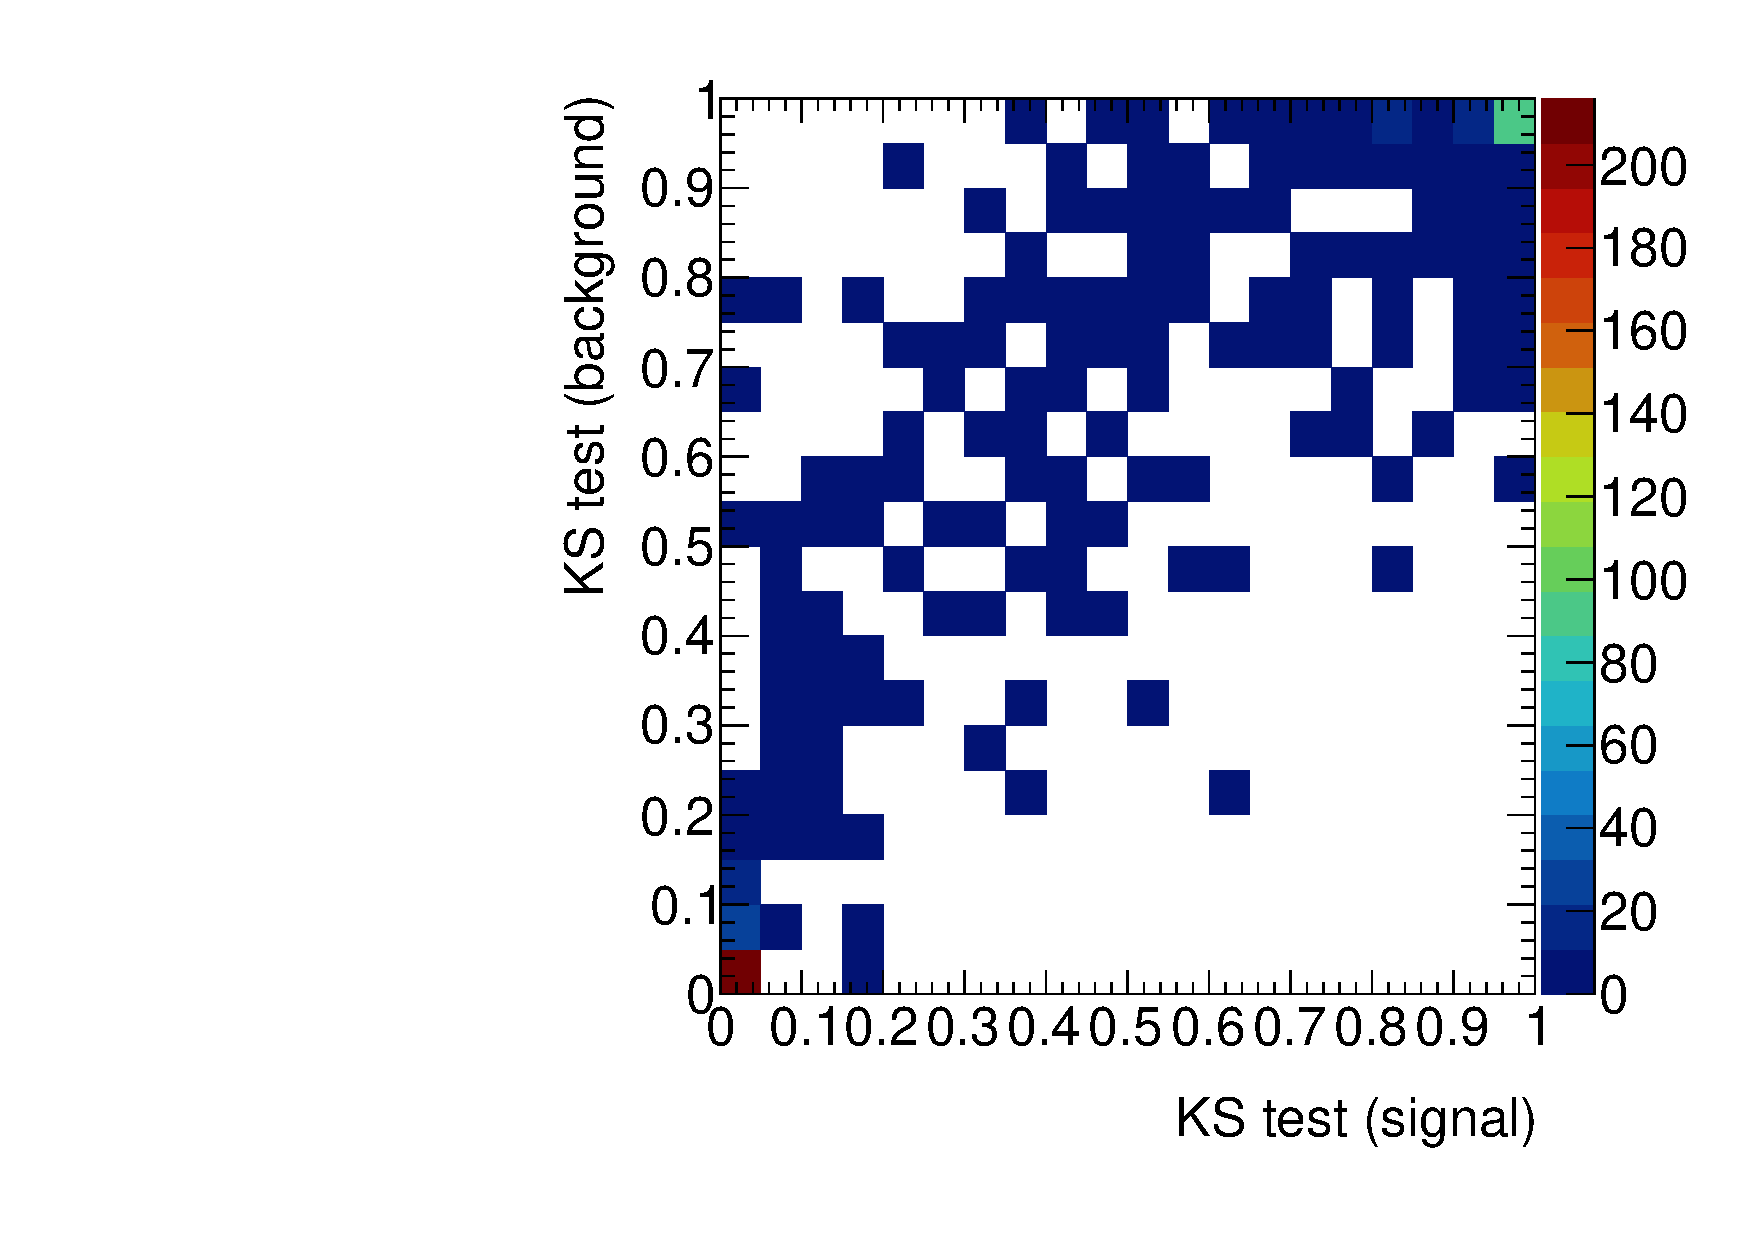
\includegraphics[width=\textwidth]{./plots/mva/scan/BOOST_DF_ks_test_sig_vs_bkg.pdf}
        \caption{Boosted DF}
    \end{subfigure}
    \caption{Correlation plots of the KS-test propability between the BDT output on the training and validaiton set for the signal and background distribution.}~\label{fig:mva:scan:kstest}
\end{figure}


The BDT with the best significance is selected for each region, the hyperparameters of the best performing BDTs are
listed in \cref{tab:mva:bestparams}.
In all regions the gradient boost algorithm is used.
The number of trees in the boosting is very similar for all regions.
Furthermore, a low maximum depth and learning rate are chosen.
There is quite some spread on the minimum number of events in the final nodes, no specific value is preferred.

The distributions of the BDT response for the four select BDTs are shown in \cref{fig:mva:scan:bdts}.
There is a very good agreement between the BDT shapes of the training and validation set.

\begin{table}[htpb]
    \centering
    \caption{Hyperparameters of the best performing BDTs in each region.}\label{tab:mva:bestparams}
    \begin{tabular}{@{}lccccc@{}}
        \toprule
        Region     & Type & NTrees & MaxDepth & MinNodeSize & LearnRate \\ \midrule
        VBF SF     & Grad & 250    & 2        & 1\,\%       & 0.1          \\
        VBF DF     & Grad & 250    & 5        & 10\,\%      & 0.05         \\
        Boosted SF & Grad & 500    & 4        & 5\,\%       & 0.05         \\
        Boosted DF & Grad & 250    & 5        & 5\,\%       & 0.1          \\
        \bottomrule
    \end{tabular}
\end{table}

\begin{figure}[htbp]
    \centering
    \begin{subfigure}[t]{0.49\textwidth}
        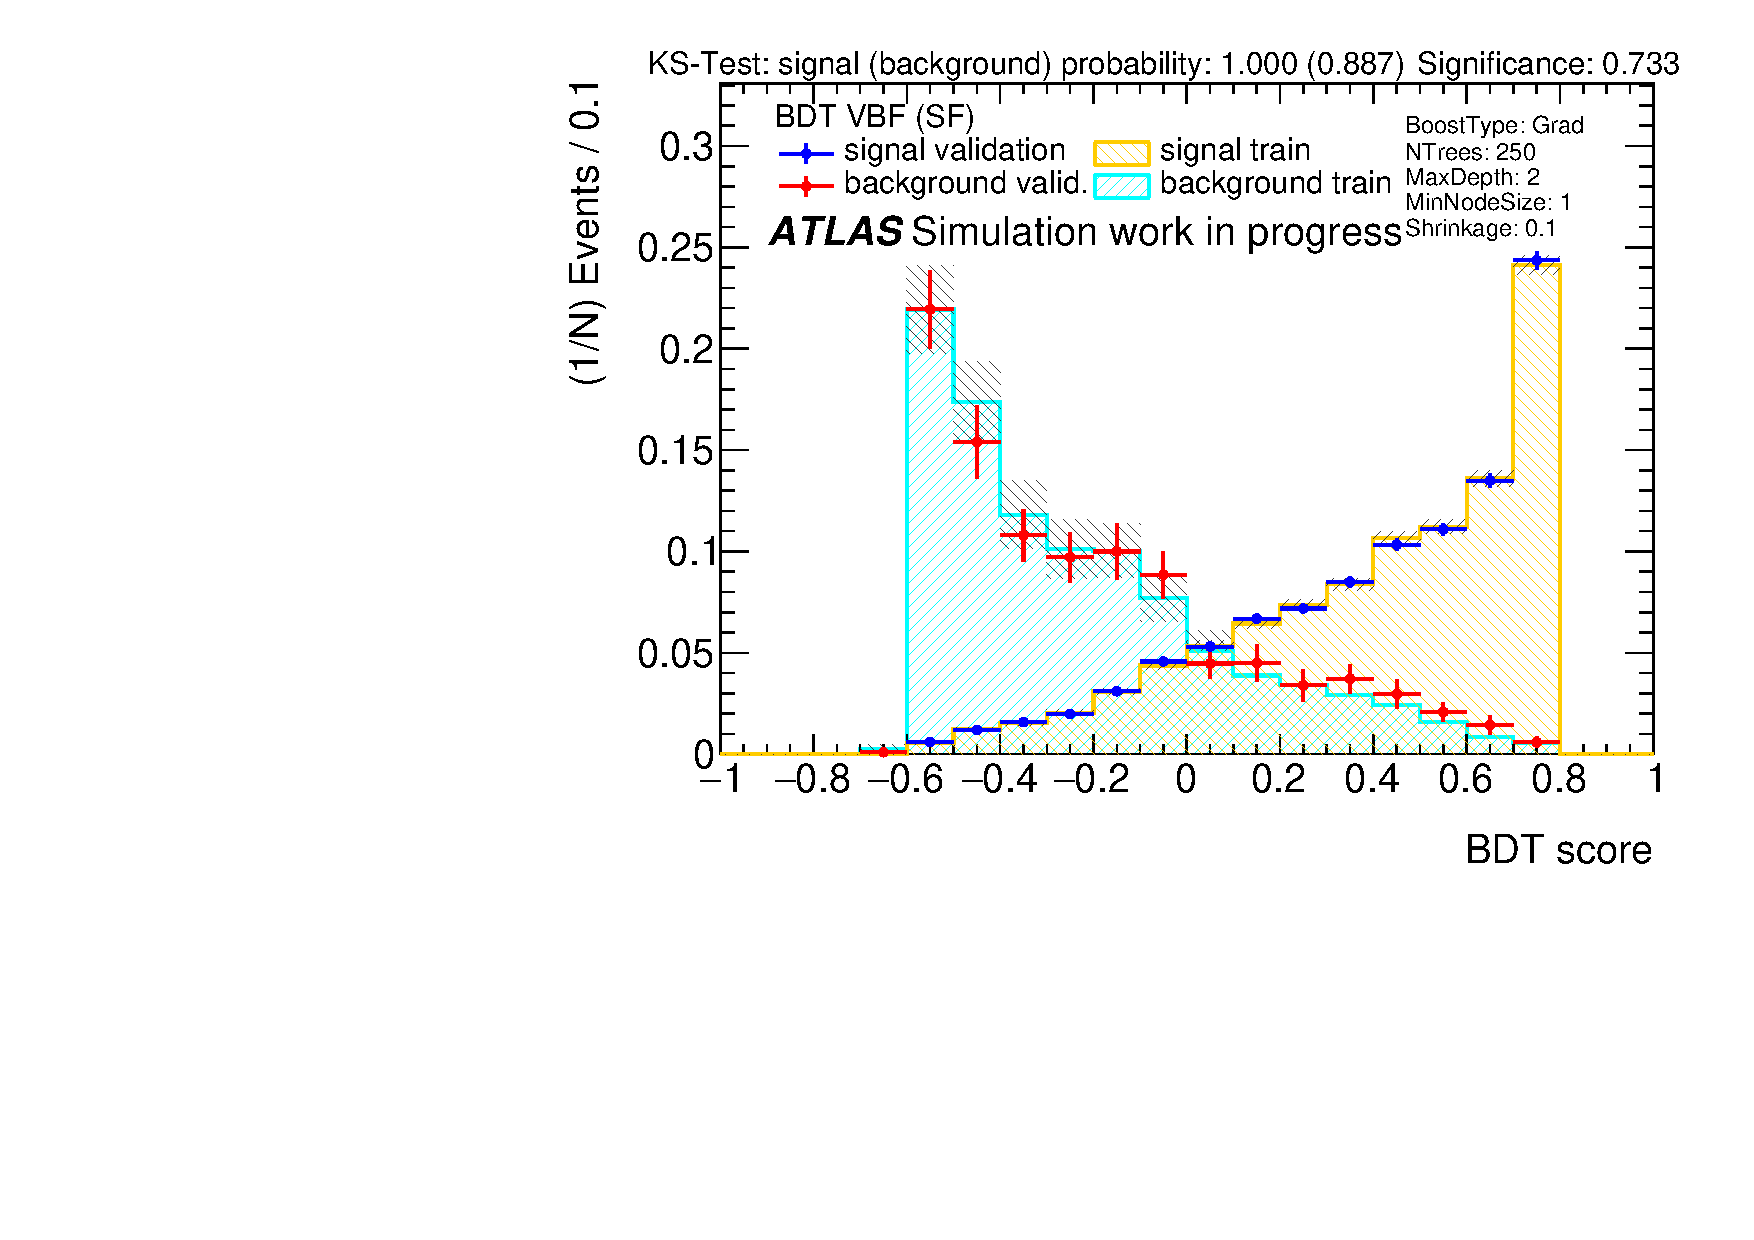
\includegraphics[width=\textwidth]{./plots/mva/scan/VBF_SF_bdt_output.pdf}
    \end{subfigure}
    \begin{subfigure}[t]{0.49\textwidth}
        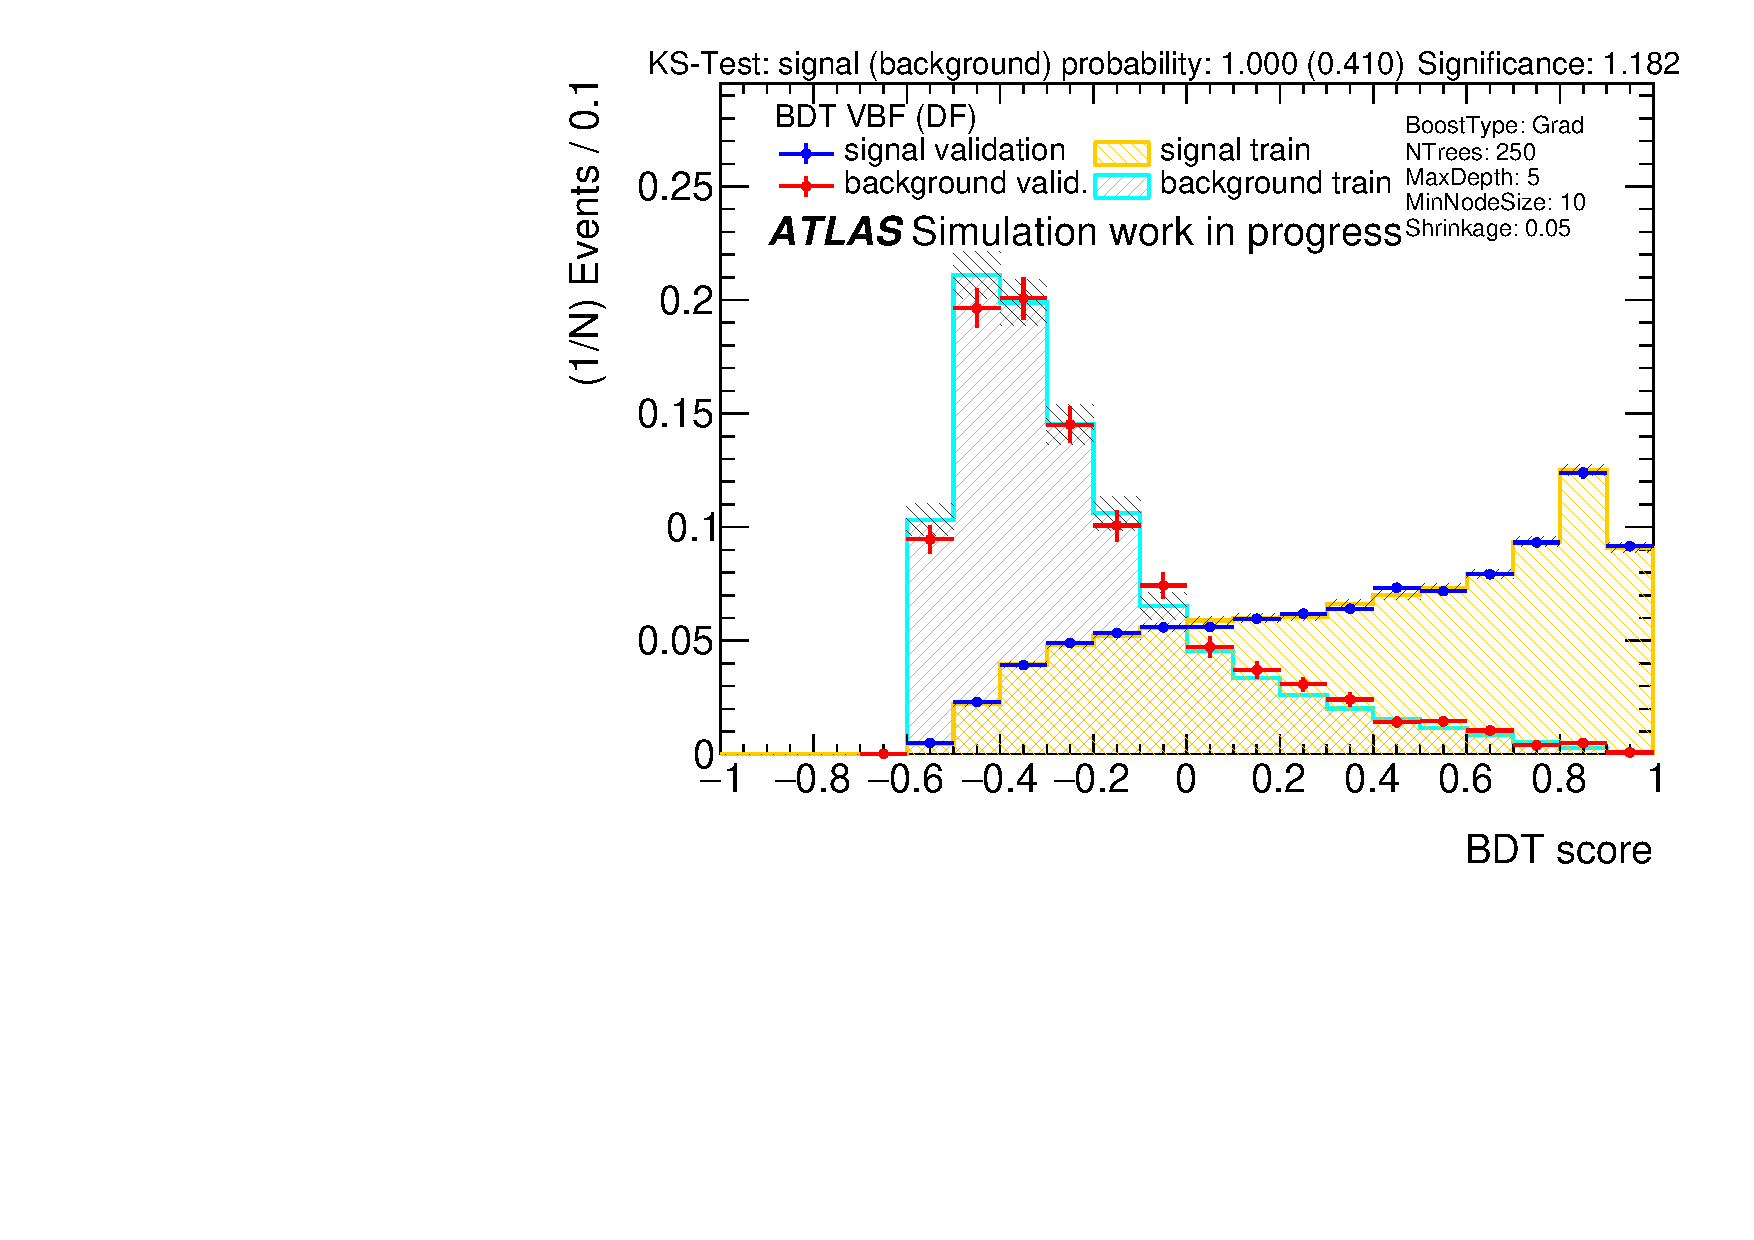
\includegraphics[width=\textwidth]{./plots/mva/scan/VBF_DF_bdt_output.pdf}
    \end{subfigure}
    \begin{subfigure}[t]{0.49\textwidth}
        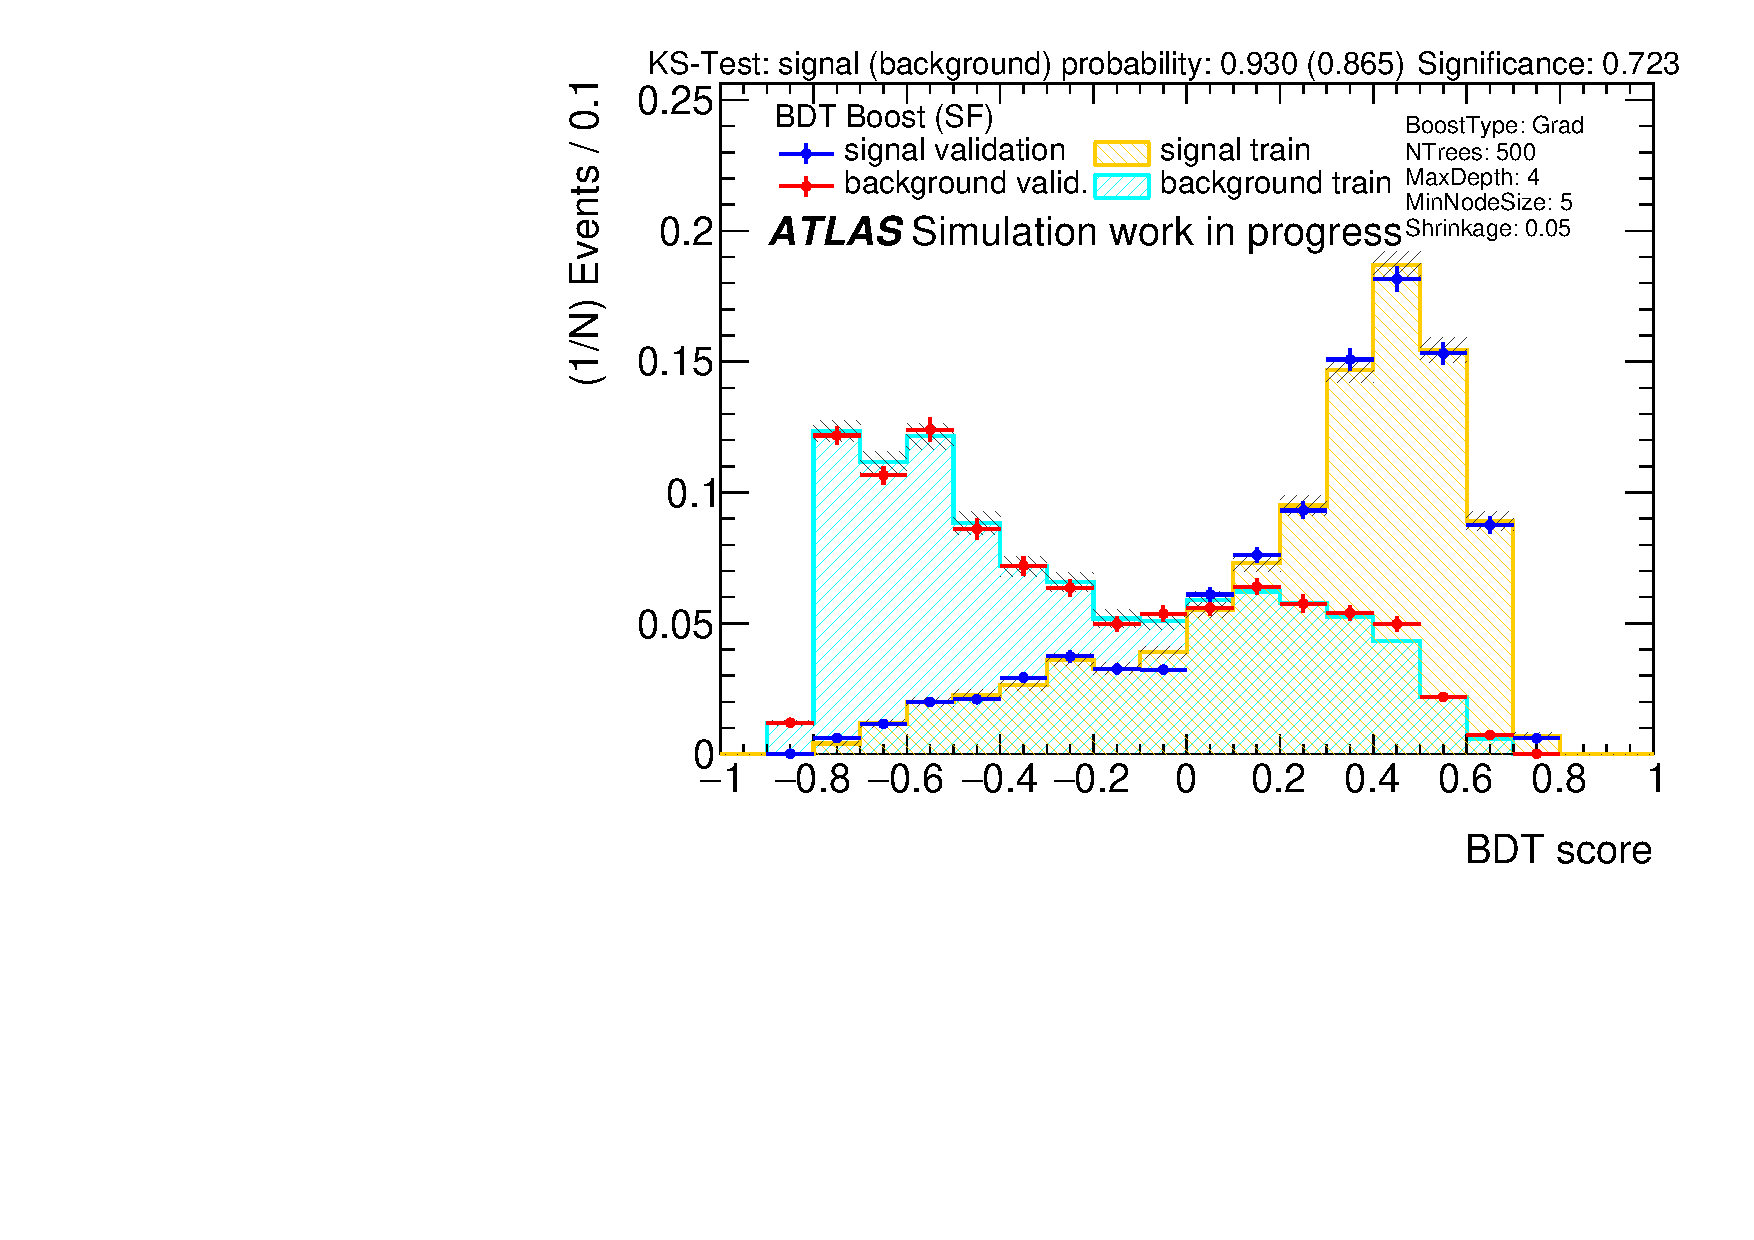
\includegraphics[width=\textwidth]{./plots/mva/scan/BOOST_SF_bdt_output.pdf}
    \end{subfigure}
    \begin{subfigure}[t]{0.49\textwidth}
        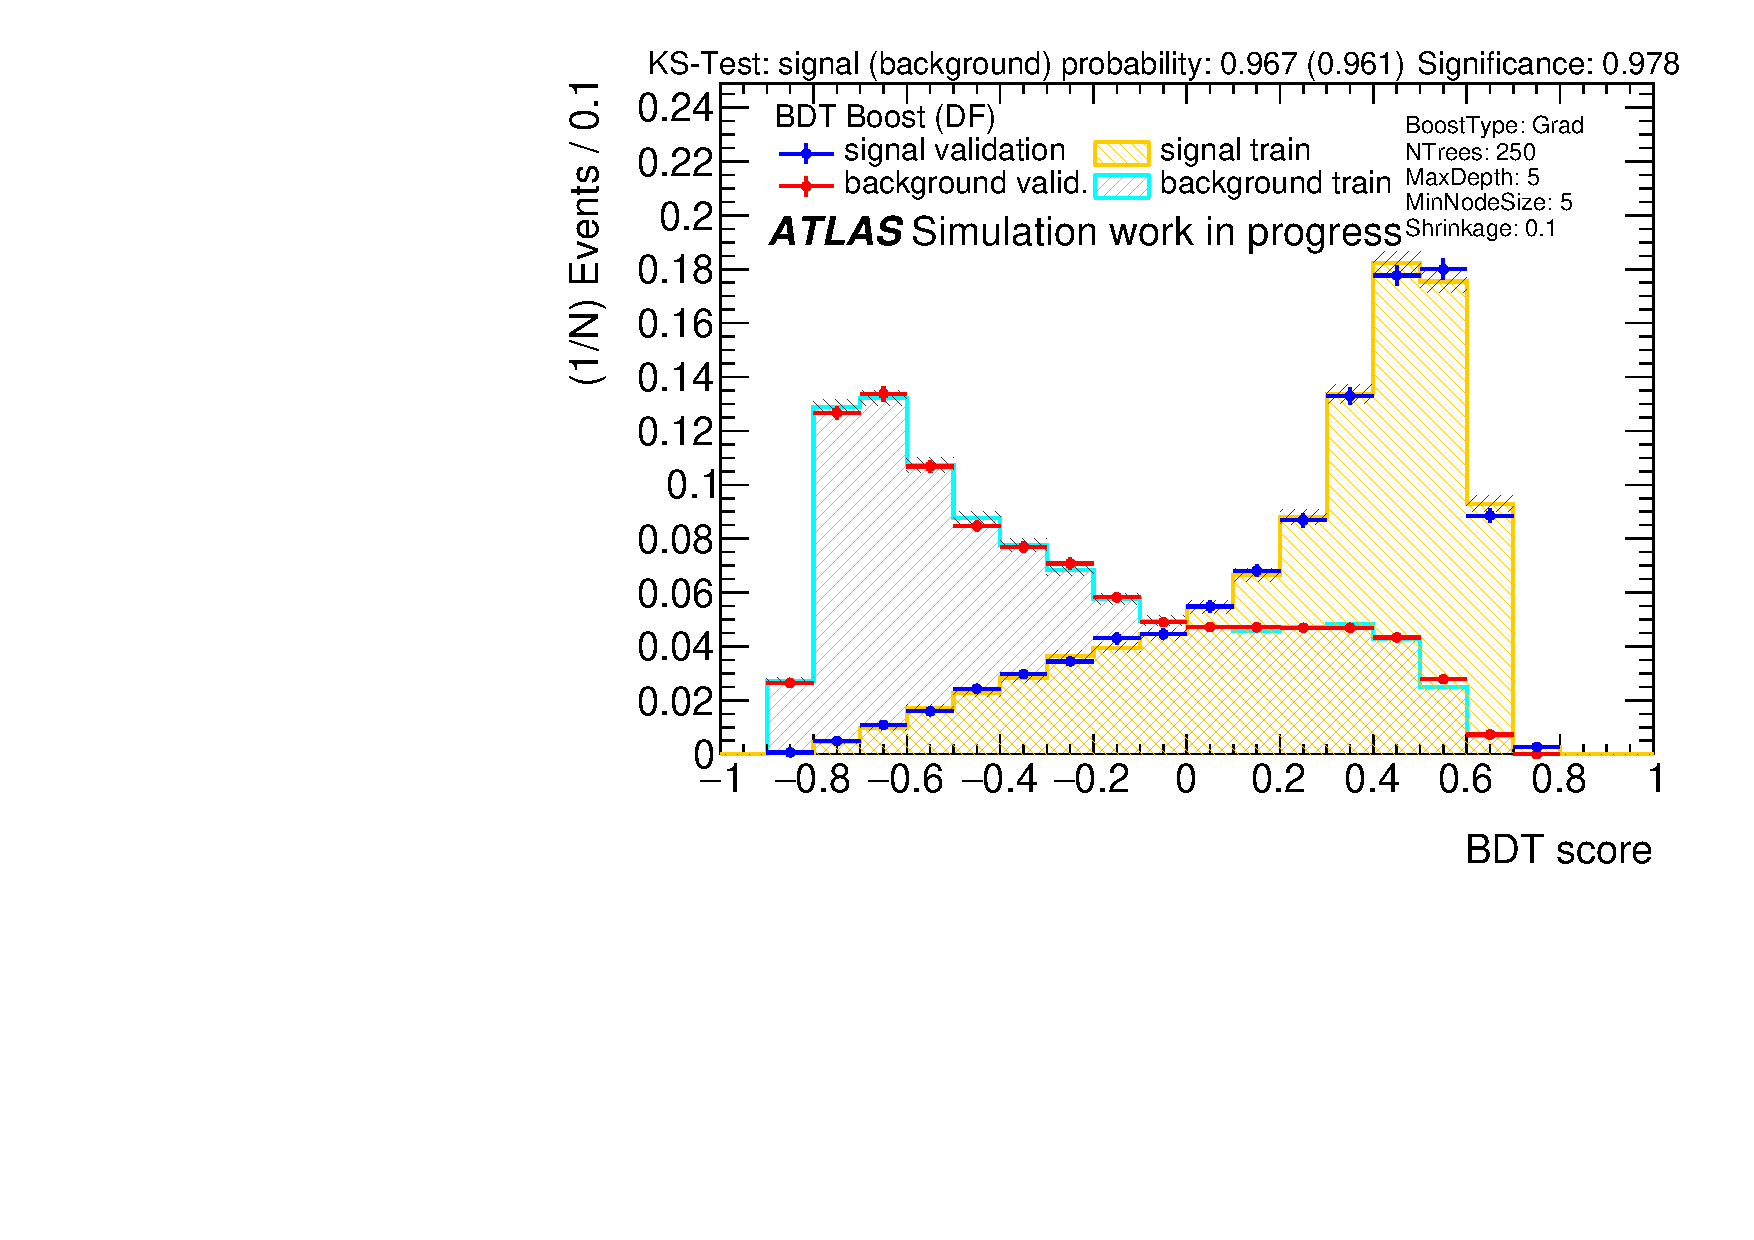
\includegraphics[width=\textwidth]{./plots/mva/scan/BOOST_DF_bdt_output.pdf}
    \end{subfigure}
    \caption{Distributions of the best performing BDTs in the hyperparameter optimization for signal and background and the training and validation set.
             The top row shows the BDTs for the VBF regions and the bottom row for the boosted regions.
             The same flavour regions are on the left and the different flavour regions on the right.
             At the top of each figure the KS-test probabilities and significances can be found.
             The areas of all distributions are normalized to one.}~\label{fig:mva:scan:bdts}
\end{figure}

\FloatBarrier{}

\subsection{Input variables}\label{sub:mva:input_variables}

Up to now the BDTs use $54$ observables as input variables.
However, a low count of input variable is desired, because the modelling of every input variable has to be reviewed.
Therefore, variables which have only a low impact on the separation power of the BDTs are discarded.
This is done individually for each region.

The impact of an input variable on the separation power of a BDT can be estimated with the so-called \emph{variable separation}.
It is calculated by counting how often a given variable is used to split a node in the decision tree while
weighting each split occurrence by the square of the gained separation $\Delta Q$ (c.f. \cref{eq:bdt:deltaQ})
and the number of events in the node~\cite{Breiman1984}.
This concept can also be used for the collection of decision trees in a boosted decision tree~\cite{TMVA}.
Variables which are not used at all have a value of zero.
A higher value indicates that the variable is more important for the performance of the BDT\@.
All variables used in a BDT are ranked by this number in a \emph{variable ranking}.
The variable ranking is averaged over all $10$ BDTs in the $k$-fold cross-evaluation.

The reduction of the number of variables is based on this variable ranking.
First, all variables which have a variable separation of zero are removed.
Then, one by one, the least performing variable is dropped from the list of input variables.
After each removal the BDT is trained again and a new variable ranking is calculated.
Additionally, the significance is calculated for each BDT as described in \cref{sub:mva:optimization:fom}.
This iterative approach is chosen, because the variable ranking can change if one ore more variables are not used anymore.

The dependence of the significance on the number of variables is shown in \cref{fig:mva:varopt:sig_vs_nvars} for each of the four regions.
As expected, the significance does not change much at first, but after removing more and more variables it decreases.
However, the curve is not always decreasing monotonically, there is some amount of statistical fluctuations caused by large event weights.
This is caused by events which were generated by the Sherpa generator~\cite{Sherpa,Gleisberg:2008fv,Cascioli:2011va,Schumann:2007mg,Hoeche:2012yf},
as described in \cref{sec:processes:mc}.
Much more simulated events are produced than expected in collisions.
To match the count of simulated and observed events, each simulated event is assigned a weight, which depends on the cross-section of the process.
Due to higher order corrections it can happen that also negative events are assigned, in the case that the cross-section of the higher order
correction is smaller than the leading order cross section. Single events which negative weights are unphysical, but combined
with a large group of other events only the decrease of the cross-section is noticeable.
There are also weights from other sources, for example from the \emph{pile-up reweighting}. These weights can have large values.
Therefore, it can happen that an event has a high negative weight.
These events cause the fluctuations in \cref{fig:mva:varopt:sig_vs_nvars}.
To reduce the amount of fluctuations the event weight is restricted to $-3 < \text{weight} < 1$ in the training and validation set.
The upper value was also included, because it turned out that also large positive event weights cause problems.

\begin{figure}[htb]
    \centering
    \begin{subfigure}[t]{0.49\textwidth}
        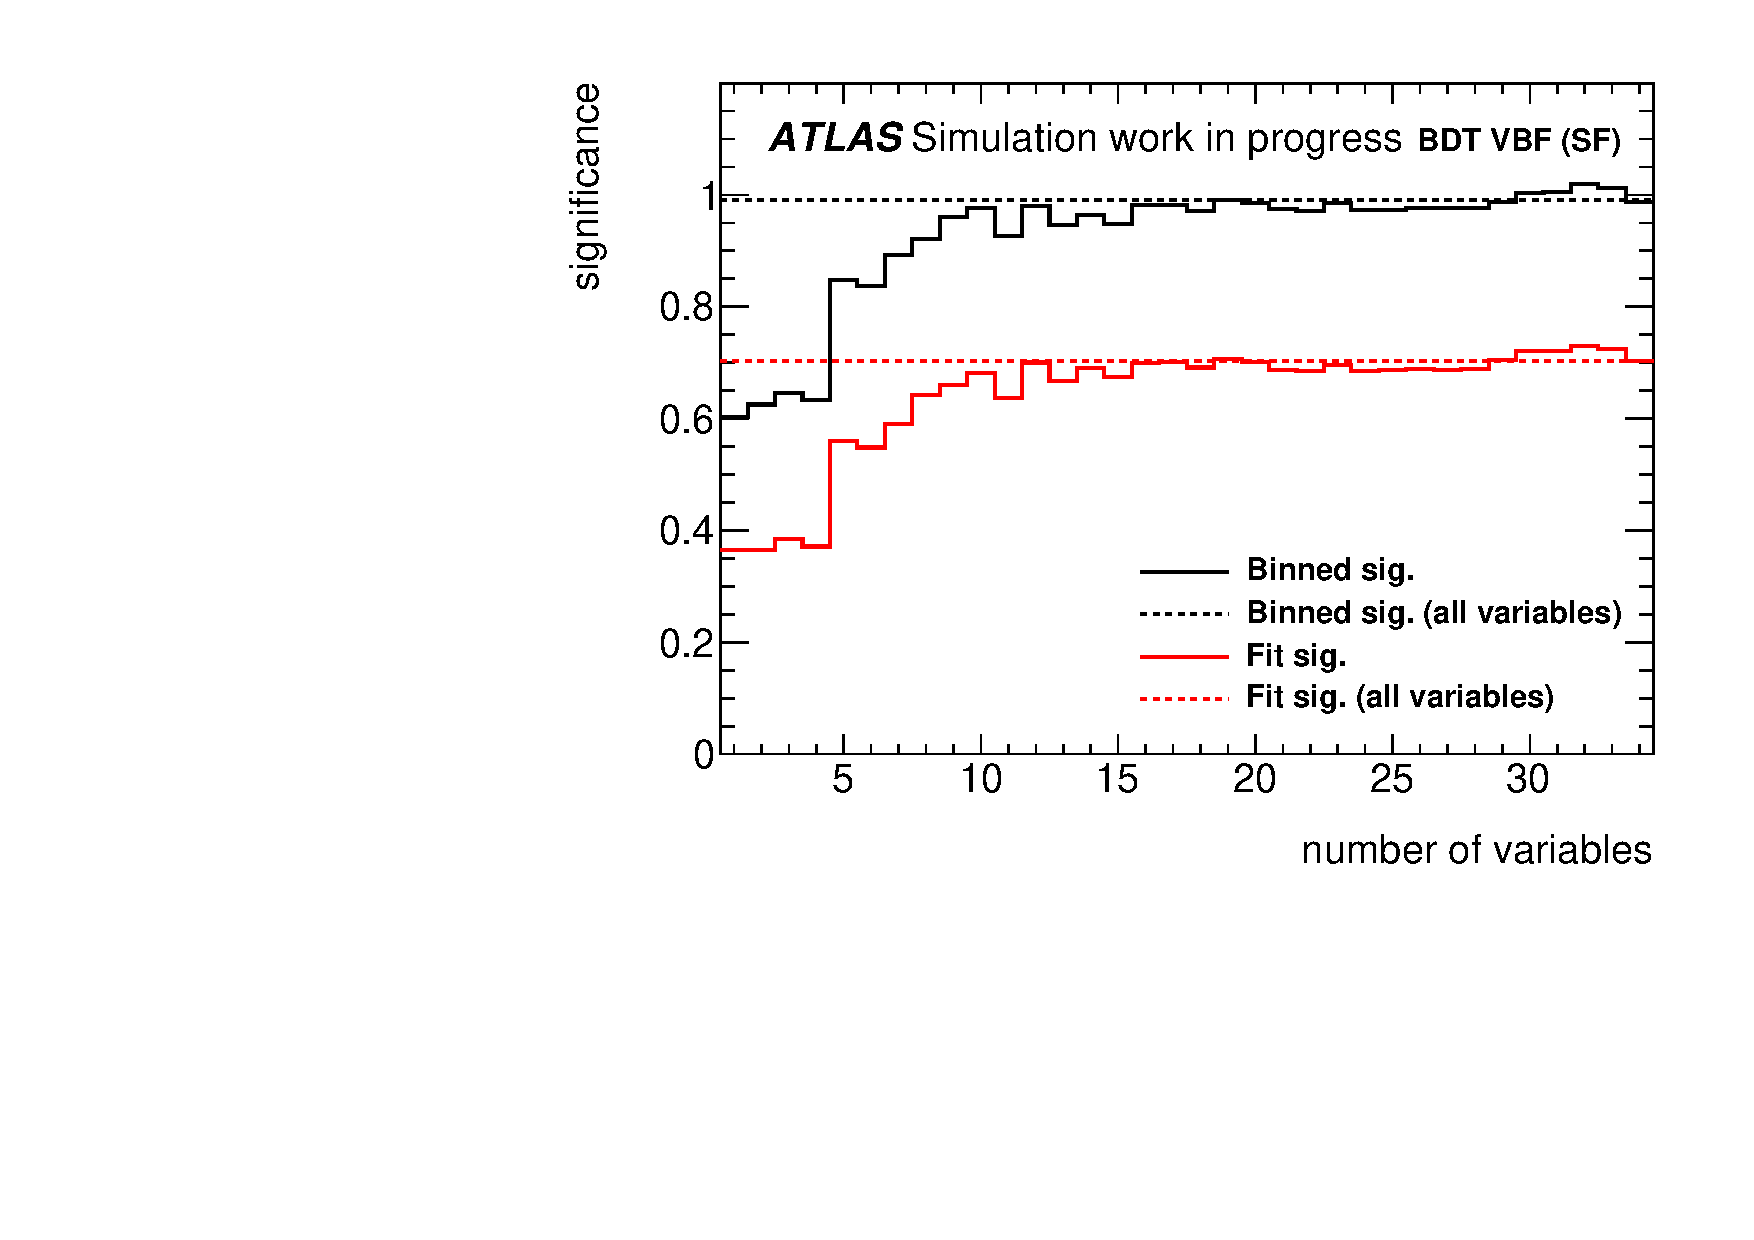
\includegraphics[width=\textwidth]{./plots/mva/variable_reduction/VBF_SF_sig_vs_nvars_all.pdf}
        \caption{VBF SF}
    \end{subfigure}
    \begin{subfigure}[t]{0.49\textwidth}
        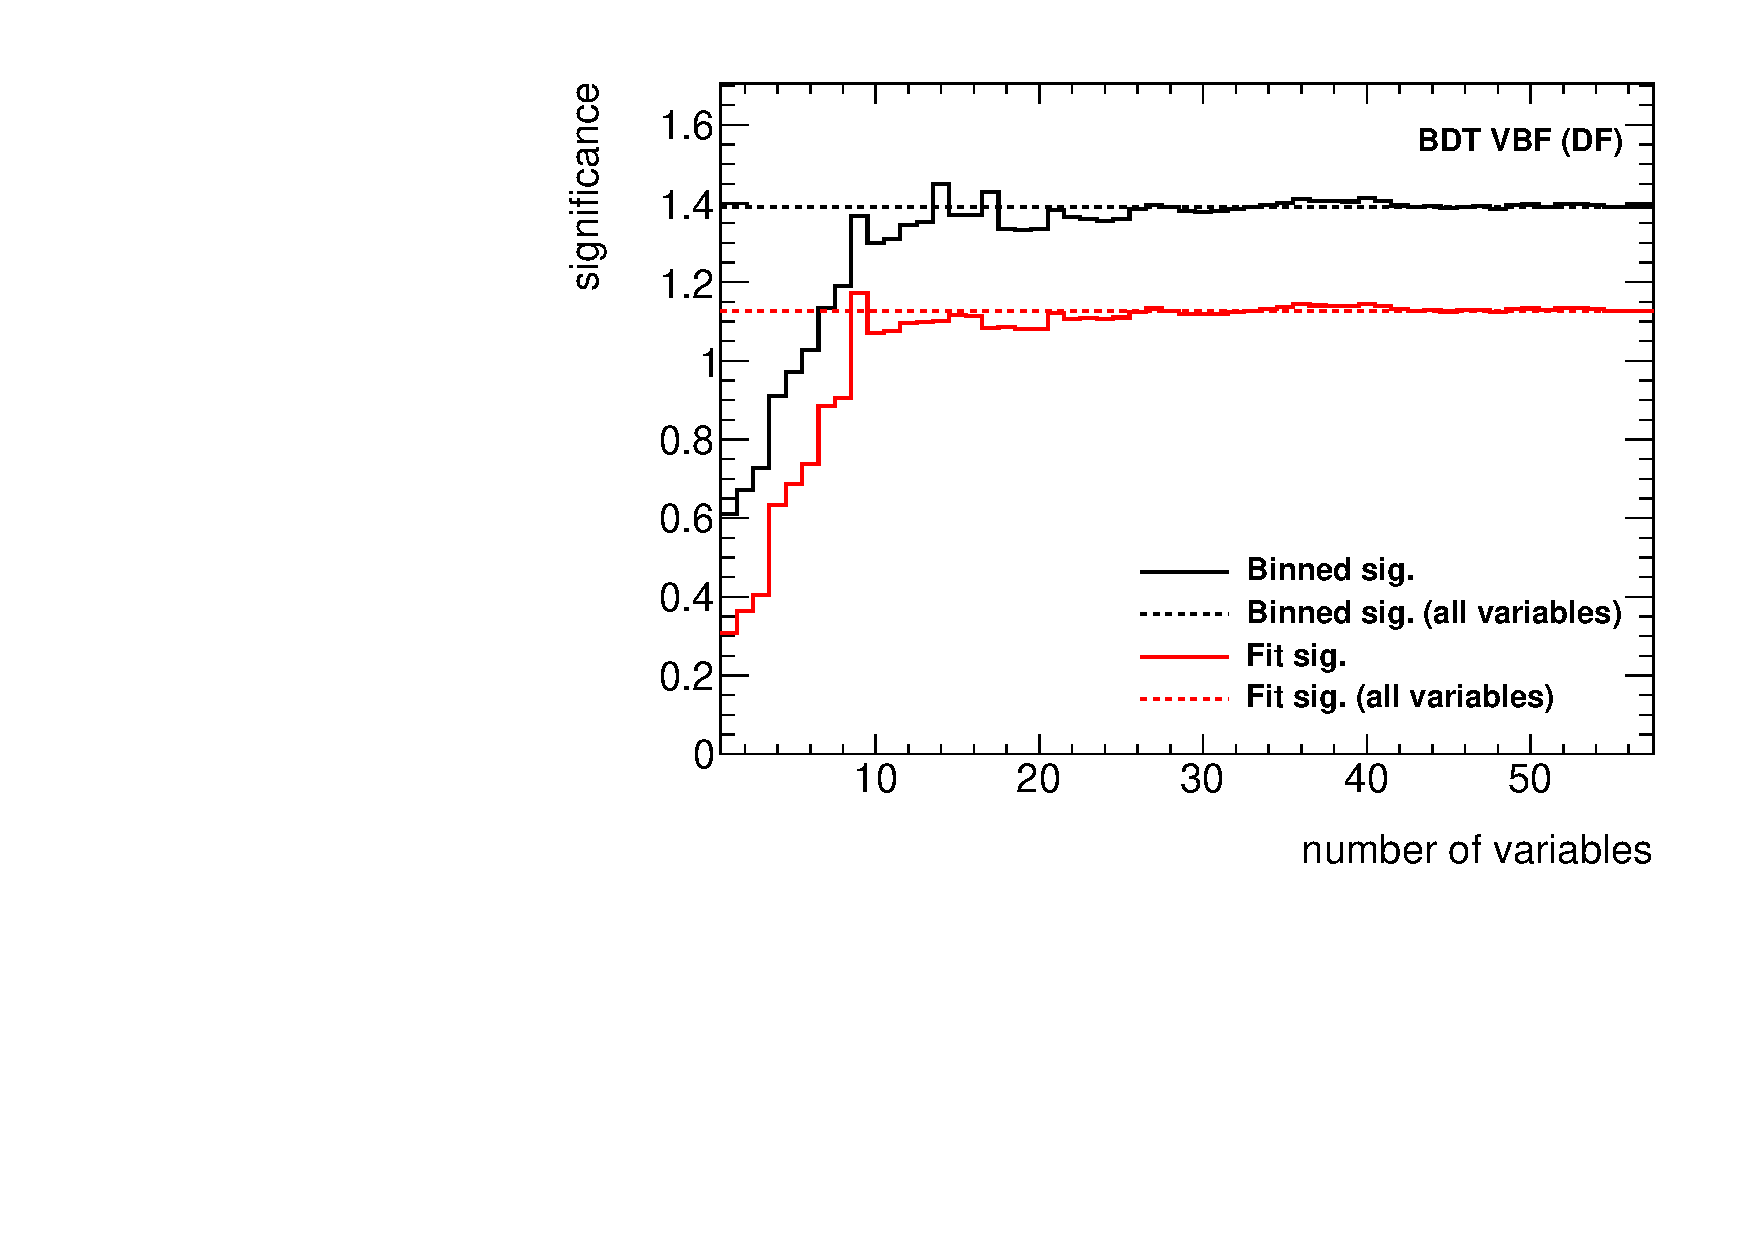
\includegraphics[width=\textwidth]{./plots/mva/variable_reduction/VBF_DF_sig_vs_nvars_all.pdf}
        \caption{VBF DF}
    \end{subfigure}
    \begin{subfigure}[t]{0.49\textwidth}
        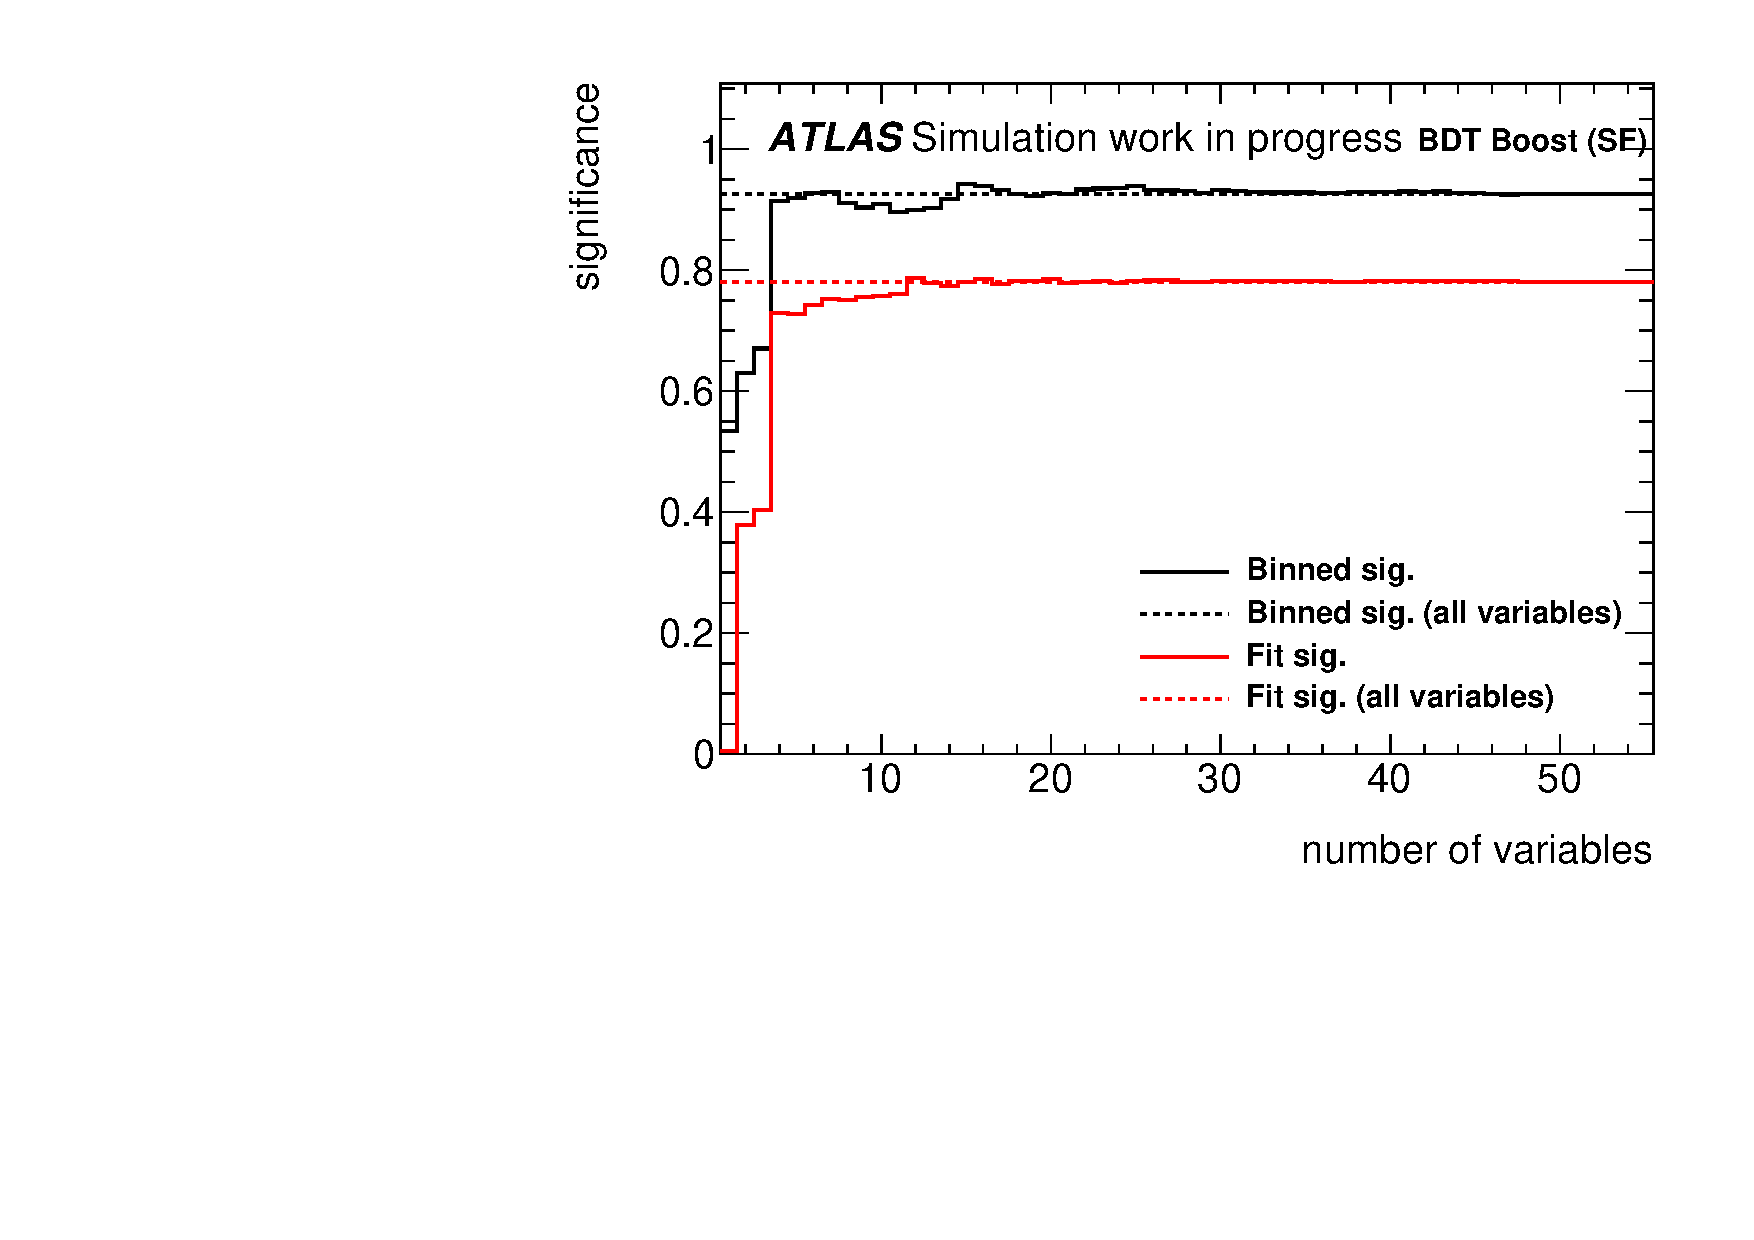
\includegraphics[width=\textwidth]{./plots/mva/variable_reduction/BOOST_SF_sig_vs_nvars_all.pdf}
        \caption{Boosted SF}
    \end{subfigure}
    \begin{subfigure}[t]{0.49\textwidth}
        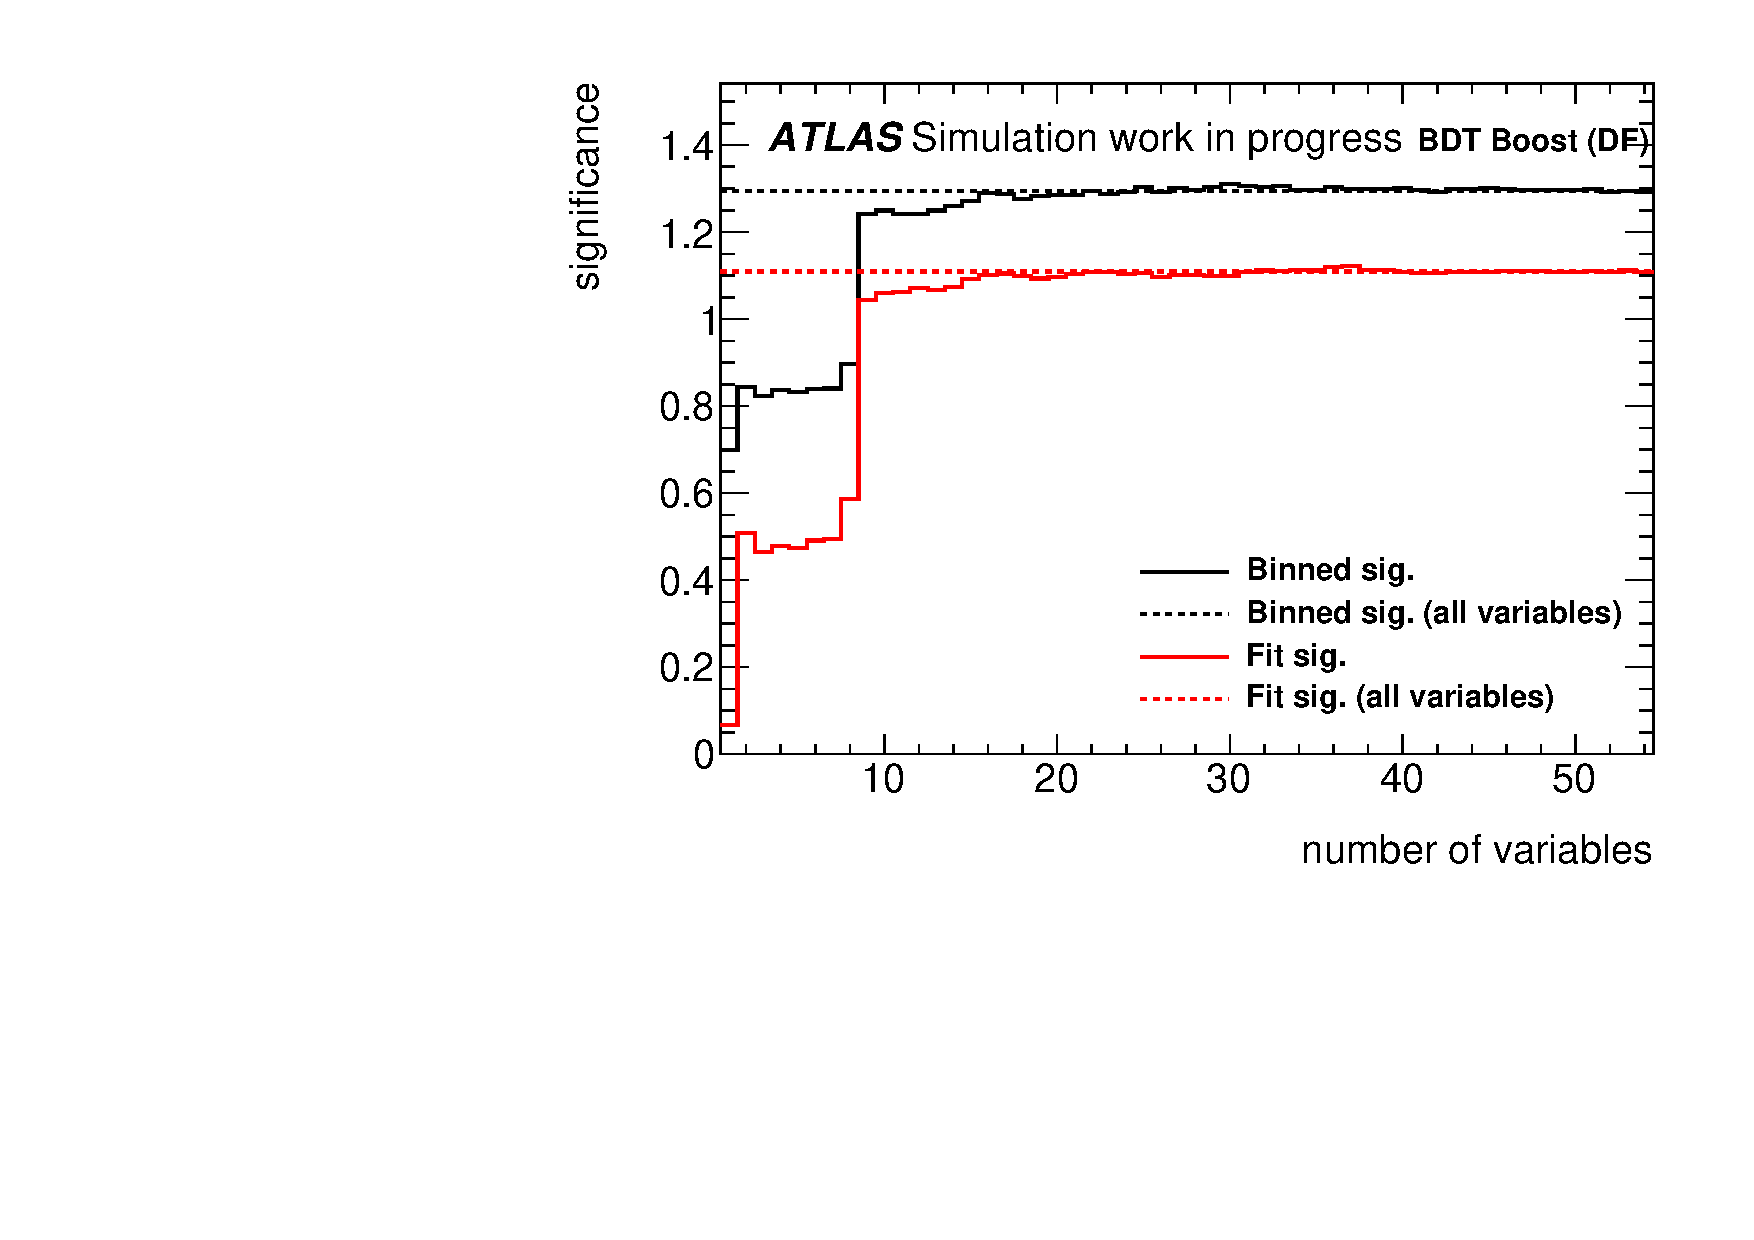
\includegraphics[width=\textwidth]{./plots/mva/variable_reduction/BOOST_DF_sig_vs_nvars_all.pdf}
        \caption{Boosted DF}
    \end{subfigure}
    \caption{Dependence of the significance on the number of input variables used in the BDT in each of the four regions.}~\label{fig:mva:varopt:sig_vs_nvars}
\end{figure}

For the BDTs in the boosted region a sharp drop-off threshold can be seen, which is used to determine the number
of input variables.
In the boosted SF and DF region $4$ and $9$ input variables is used, respectively.
The decision how much variables in the VBF regions should be used was more difficult, because there is not such a clear drop-off in the expected significance.
A trade-off between the decrease of significance and remaining count of variables has to be made.
In the end, $9$ variables were chosen for the VBF SF region and $8$ for the VBF DF region.
The chosen observables are discussed below.
Not all observable are used in every region.
The variable rankings can be found in \cref{tab:mva:variables:ranking:VBFSF,tab:mva:variables:ranking:VBFDF,tab:mva:variables:ranking:BOOSTSF,tab:mva:variables:ranking:BOOSTDF}
Distributions of all variables are shown in the next section.

\begin{table}[htpb]
    \centering
    \caption{Variable ranking for the final BDT in the VBF SF region calculated by averaging over the individual
             variable rankings of the $10$ BDTs from the $k$-fold cross-validation.}\label{tab:mva:variables:ranking:VBFSF}
    \begin{tabular}{rlcc}
        \toprule
        Rank & Observable & Mean Variable Separation & Standard Deviation \\ \midrule
        1 & $\drll$ & 0.212 & 0.016 \\
        2 & $\mmc$ & 0.178 & 0.015 \\
        3 & $\min \Delta R (\ell\ell, \text{jets})$ & 0.154 & 0.014 \\
        4 & $\mjj$ & 0.130 & 0.014 \\
        5 & $\min \Delta R (\ell_2, \text{jets})$ & 0.098 & 0.018 \\
        6 & $n_\text{jets}$ & 0.089 & 0.007 \\
        7 & $\etmiss \phi$ centrality & 0.080 & 0.011 \\
        8 & $\pt^\text{total}$ & 0.053 & 0.025 \\
        9 & $\etmiss$ & 0.005 & 0.007 \\
        \bottomrule
    \end{tabular}
\end{table}

\begin{table}[htpb]
    \centering
    \caption{Variable ranking for the final BDT in the VBF DF region calculated by averaging over the individual
             variable rankings of the $10$ BDTs from the $k$-fold cross-validation.}\label{tab:mva:variables:ranking:VBFDF}
    \begin{tabular}{rlcc}
        \toprule
        Rank & Observable & Mean Variable Separation & Standard Deviation \\ \midrule
        1 & $\drll$ & 0.180 & 0.009 \\
        2 & $\min \Delta R (\ell\ell, \text{jets})$ & 0.165 & 0.009 \\
        3 & $\etmiss \phi$ centrality & 0.144 & 0.009 \\
        4 & $\mmc$ & 0.132 & 0.014 \\
        5 & $\min \Delta R (\ell_2, \text{jets})$ & 0.129 & 0.010 \\
        6 & $\mjj$ & 0.112 & 0.011 \\
        7 & $\pt^\text{total}$ & 0.090 & 0.017 \\
        8 & $n_\text{jets}$ & 0.048 & 0.009 \\
        \bottomrule
    \end{tabular}
\end{table}
\begin{table}[htpb]
    \centering
    \caption{Variable ranking for the final BDT in the boosted SF region calculated by averaging over the individual
             variable rankings of the $10$ BDTs from the $k$-fold cross-validation.}\label{tab:mva:variables:ranking:BOOSTSF}
    \begin{tabular}{rlcc}
        \toprule
        Rank & Observable & Mean Variable Separation & Standard Deviation \\ \midrule
        1 & $\mmc$ & 0.446 & 0.038 \\
        2 & $\drll$ & 0.238 & 0.031 \\
        3 & $\mll$ & 0.227 & 0.019 \\
        4 & $\etmiss$ & 0.089 & 0.017 \\
        \bottomrule
    \end{tabular}
\end{table}
\begin{table}[htpb]
    \centering
    \caption{Variable ranking for the final BDT in the boosted DF region calculated by averaging over the individual
             variable rankings of the $10$ BDTs from the $k$-fold cross-validation.}\label{tab:mva:variables:ranking:BOOSTDF}
    \begin{tabular}{rlcc}
        \toprule
        Rank & Observable & Mean Variable Separation & Standard Deviation \\ \midrule
        1 & $\mmc$ & 0.263 & 0.007 \\
        2 & $m_\text{T}^{\ell_0}$ & 0.115 & 0.009 \\
        3 & $\min \Delta R (\ell\ell, \text{jets})$ & 0.107 & 0.007 \\
        4 & $\mll$ & 0.107 & 0.010 \\
        5 & $m_{\tau\tau,\text{j}_1}$ & 0.097 & 0.006 \\
        6 & $\drll$ & 0.085 & 0.009 \\
        7 & $\etmiss / \pt^{\ell_2}$ & 0.078 & 0.015 \\
        8 & Sphericity & 0.075 & 0.004 \\
        9 & $\eta_{\ell_1}$ & 0.074 & 0.009 \\
        \bottomrule
    \end{tabular}
\end{table}


\subsubsection{Common observables}
The following variables are used in both the VBF and boosted category.
\begin{itemize}
    \item The mass of the missing mass calculator, $\mmc$, as discussed in \cref{sub:event_selection:mmc}.
    \item The missing transverse energy, $\etmiss$, as defined in \cref{sec:object_selection:missing_transverse_energy}.
    \item The minimum $\Delta \eta$ distance between the dilepton system and all jets, $\min \Delta \eta (\ell\ell, \text{jets})$.
        This observable is not used in BDTs of the boosted SF region.
    \item The $\Delta R$ as defined in \cref{eq:deltar} between the two leptons, $\drll$.
\end{itemize}


\subsubsection{VBF category specific observables}
The following variables are only used in the VBF category.
\begin{itemize}
    \item The mass of the dijet system of the two leading jets, $\mjj$.
    \item The number of jets. For the counting only jets with $\pt > \SI{30}{\GeV}$ are used.
          Only a distinction between events with two jets and more than two jets is made, since high jet-multiplicity bins
          have only leading order precision.
    \item The $\etmiss \phi$ centrality, which quantifies the centrality of the $\etmissvec$ vector with respect to the final
          state leptons in the transverse plane.
          The transverse plane is orthogonal to the direction of both final state leptons. The smaller $\phi$ angle between
          the two leptons defines the positive quadrant.
          The $\phi$ centrality, $C_\phi(\ell\ell,k)$, is calculated for an object $k$ by~\cite{SchilloPhd}
          \begin{align}
              \label{eq:mva:metphicentrality}
              C_\phi^A(\ell\ell,k) &= \sin(\phi_k - \phi_{\ell_1}) / \sin(\phi_{\ell_2} - \phi_{\ell_1}) \\
              C_\phi^B(\ell\ell,k) &= \sin(\phi_{\ell_2} - \phi_k) / \sin(\phi_{\ell_2} - \phi_{\ell_1}) \\
              C_\phi(\ell\ell,k) &=  \frac{C_\phi^A(\ell\ell,k) + C_\phi^B(\ell\ell,k)}{\sqrt{C_\phi^A{(\ell\ell,k)}^2 + C_\phi^B{(\ell\ell,k)}^2}}
          \end{align}
    \item The norm of the vectorial sum of the transverse momentum of the two final state leptons, the two leading jets, and the missing transverse energy, $\pt^\text{total}$.
    \item The minimum distance in $\Delta R$ between the leading lepton and all jets, $\min \Delta \eta (\ell_1, \text{jets})$.
            This observable is only used in the BDTs of the VBF DF region.
    \item The minimum distance in $\Delta R$ between the subleading lepton and all jets, $\min \Delta \eta (\ell_2, \text{jets})$.
            This observable is only used in the BDTs of the VBF SF region.
\end{itemize}

\subsubsection{Boosted category specific observables}
The following variables are only used in the boosted category.
\begin{itemize}
    \item The mass of the dilepton system, $\mll$.
    \item The sum of the mass of the visible decay products of the $\tau$-lepton decay and the mass of the leading jet, $m_{\tau\tau,\text{j}_1} $.
    \item The fraction of the missing transverse energy and the transverse momentum of the second jet, $\etmiss / \pt^{\ell_2}$.
        This observable is only used in the BDTs of the boosted DF region.
    \item The sphericity, a measure for the isotropy of the energy flow in the event~\cite{Sphericity}.
          First, the momentum tensor of all selected leptons and jets in the event is calculated,
          \begin{equation}
              S^{\alpha\beta} = \frac{\sum_i p_i^\alpha p_i^\beta}{\sum_i \abs{\vec{p}_i^2}} \qquad \alpha, \beta = 1,2, 3 \,.
          \end{equation}
          The sphericity $S$ is then built from the two smallest eigenvalues $\lambda_2$ and $\lambda_3$ of this vector,
          \begin{equation}
              \label{eq:mva:sphericity}
              S = \frac{3}{2} \left( \lambda_2 + \lambda_3 \right) \,.
          \end{equation}
    \item The transverse mass of the leading lepton with the missing transverse energy, $m_\text{T}^{\ell_1}$.
        This observable is only used in the BDTs of the boosted DF region.
    \item The pseudorapidity of the leading lepton, $\eta_{\ell_1}$.
        This observable is only used in the BDTs of the boosted DF region.
\end{itemize}


\subsubsection{Final BDT distributions}

The BDT distributions of the final BDTs are shown in \cref{fig:mva:varopt:bdts} for training and validation set.
There is an excellent agreement between the distributions of the training and validation set for both signal and background.
The correlation plots of the input variables can be found in \cref{app:mva:correlation_inputvars}.

\begin{figure}[htbp]
    \centering
    \begin{subfigure}[t]{0.49\textwidth}
        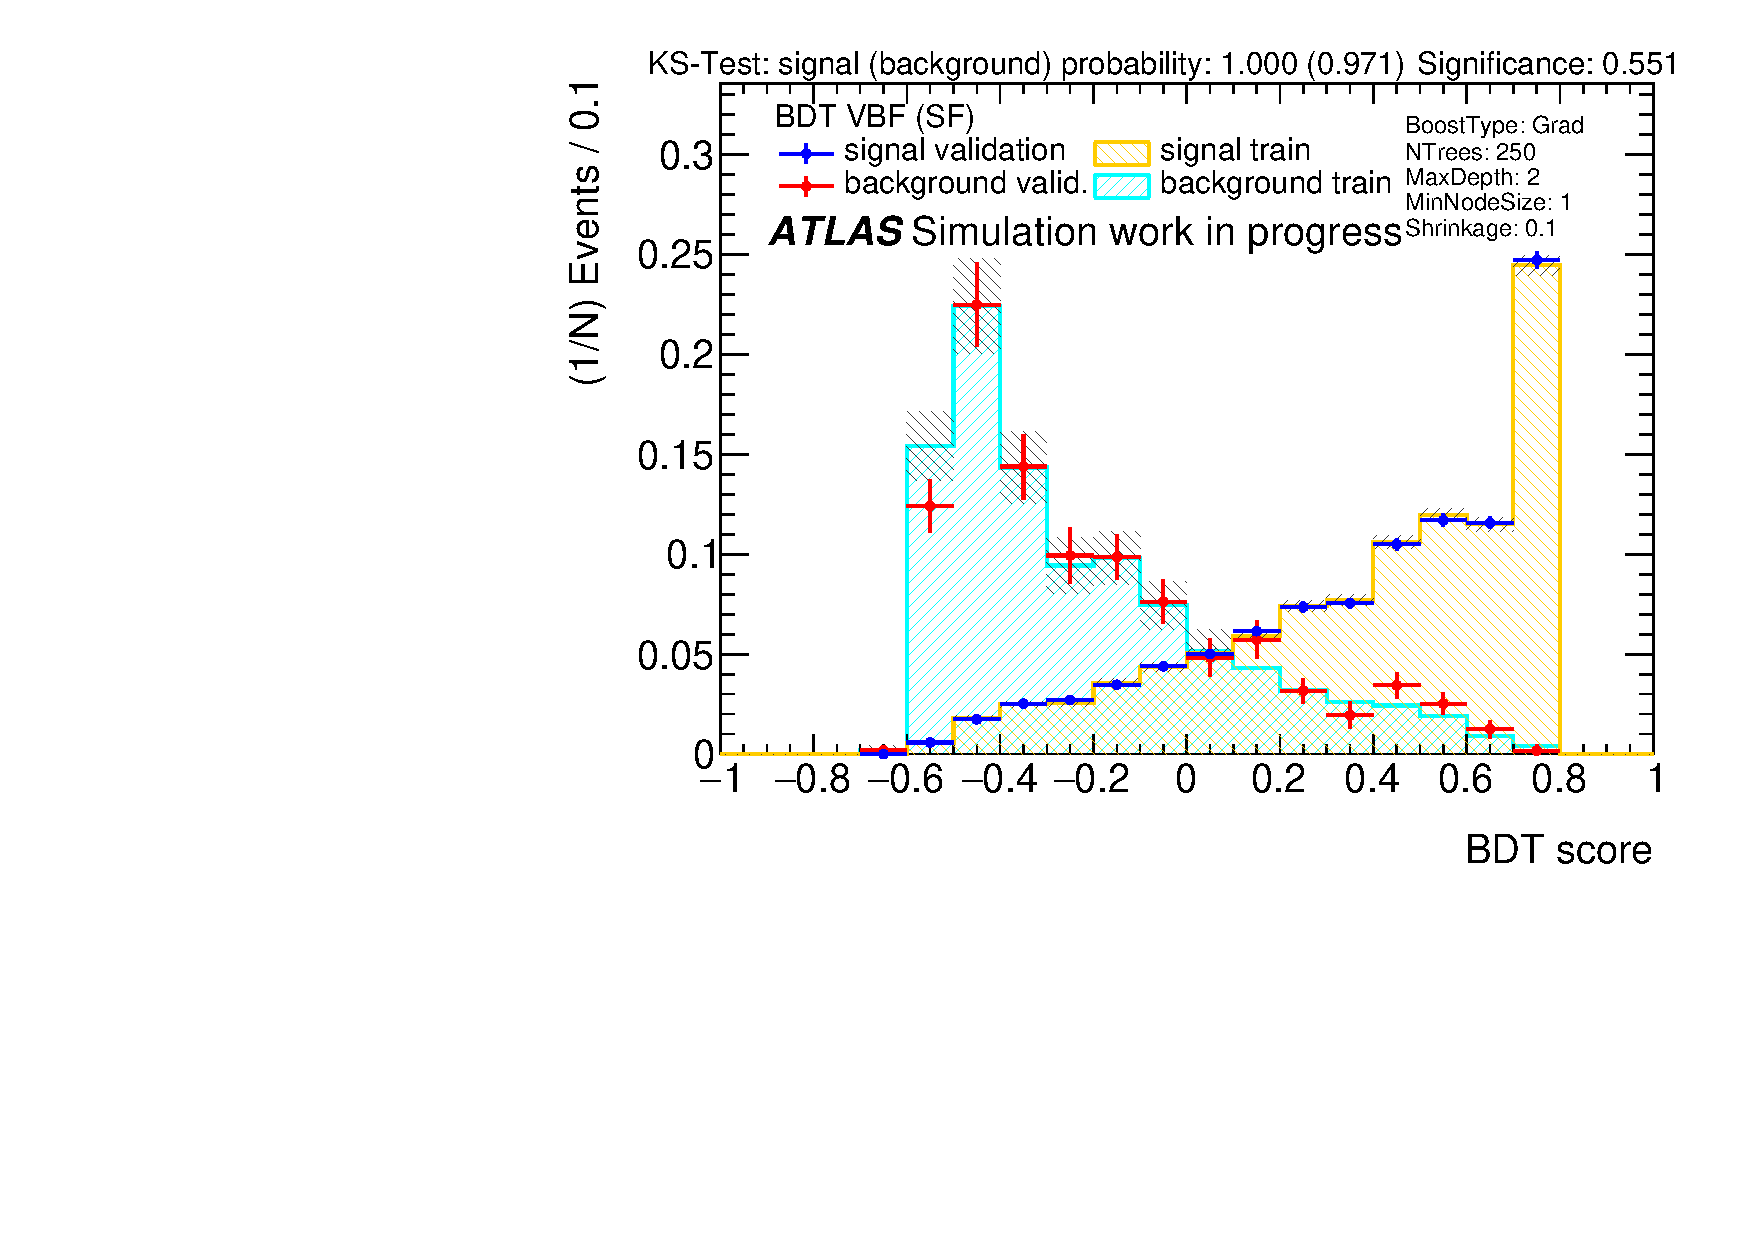
\includegraphics[width=\textwidth]{./plots/mva/variable_reduction/VBF_SF_bdt_output_clean.pdf}
    \end{subfigure}
    \begin{subfigure}[t]{0.49\textwidth}
        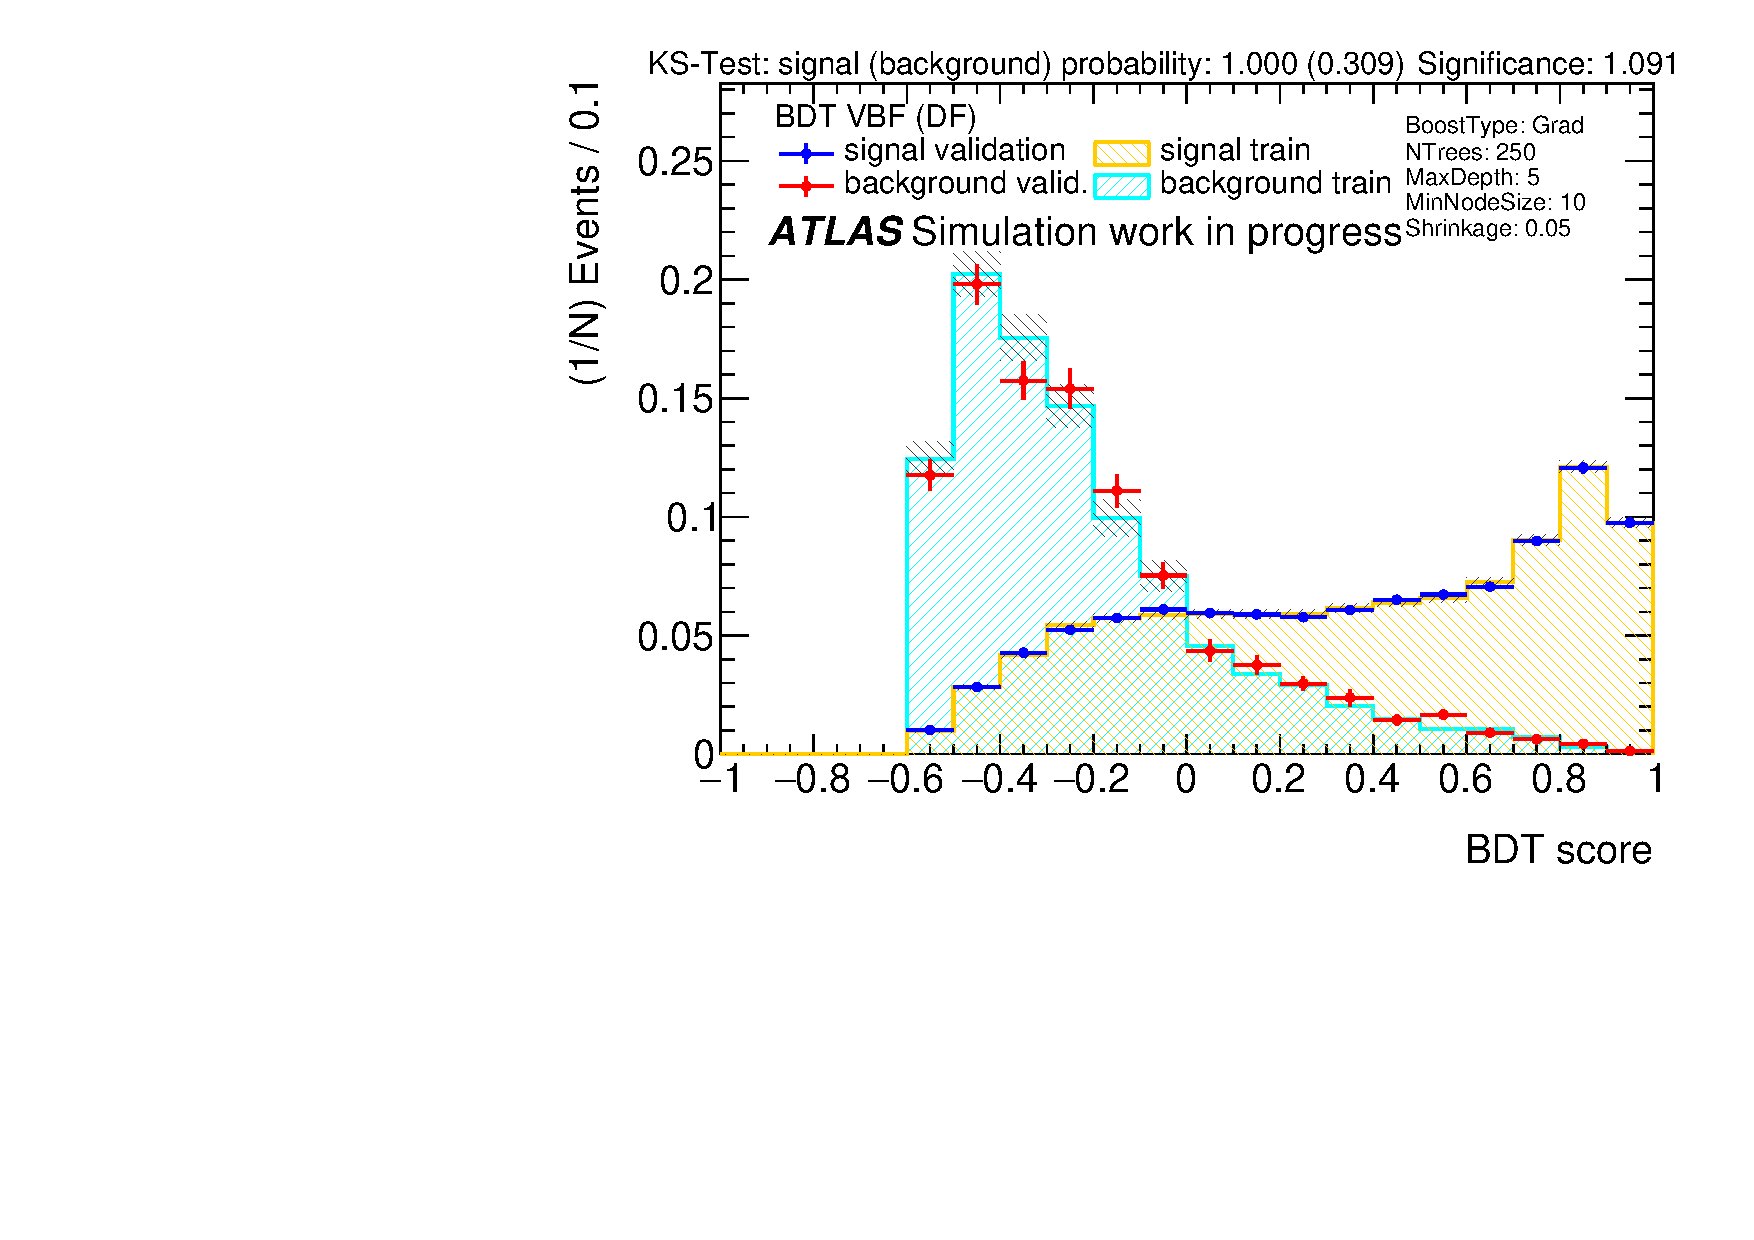
\includegraphics[width=\textwidth]{./plots/mva/variable_reduction/VBF_DF_bdt_output_clean.pdf}
    \end{subfigure}
    \begin{subfigure}[t]{0.49\textwidth}
        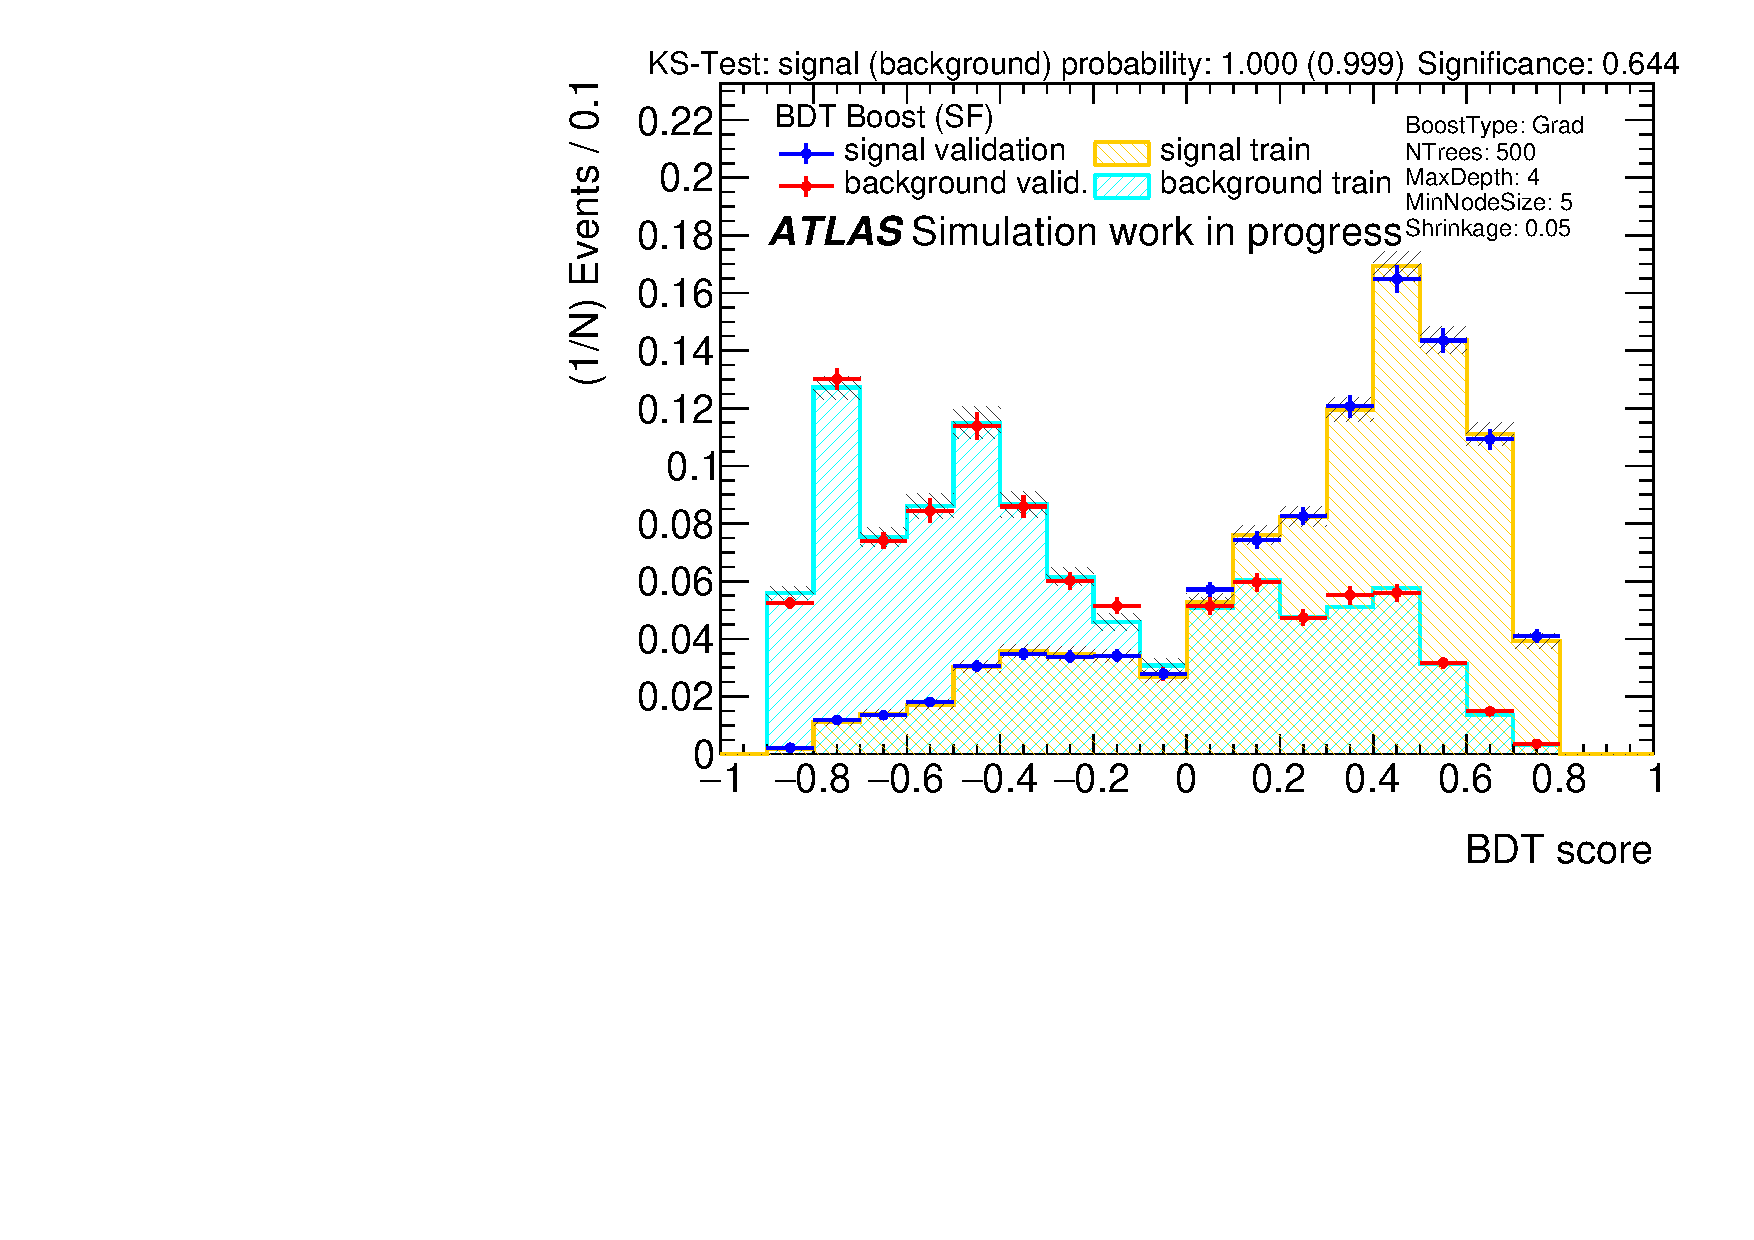
\includegraphics[width=\textwidth]{./plots/mva/variable_reduction/BOOST_SF_bdt_output_clean.pdf}
    \end{subfigure}
    \begin{subfigure}[t]{0.49\textwidth}
        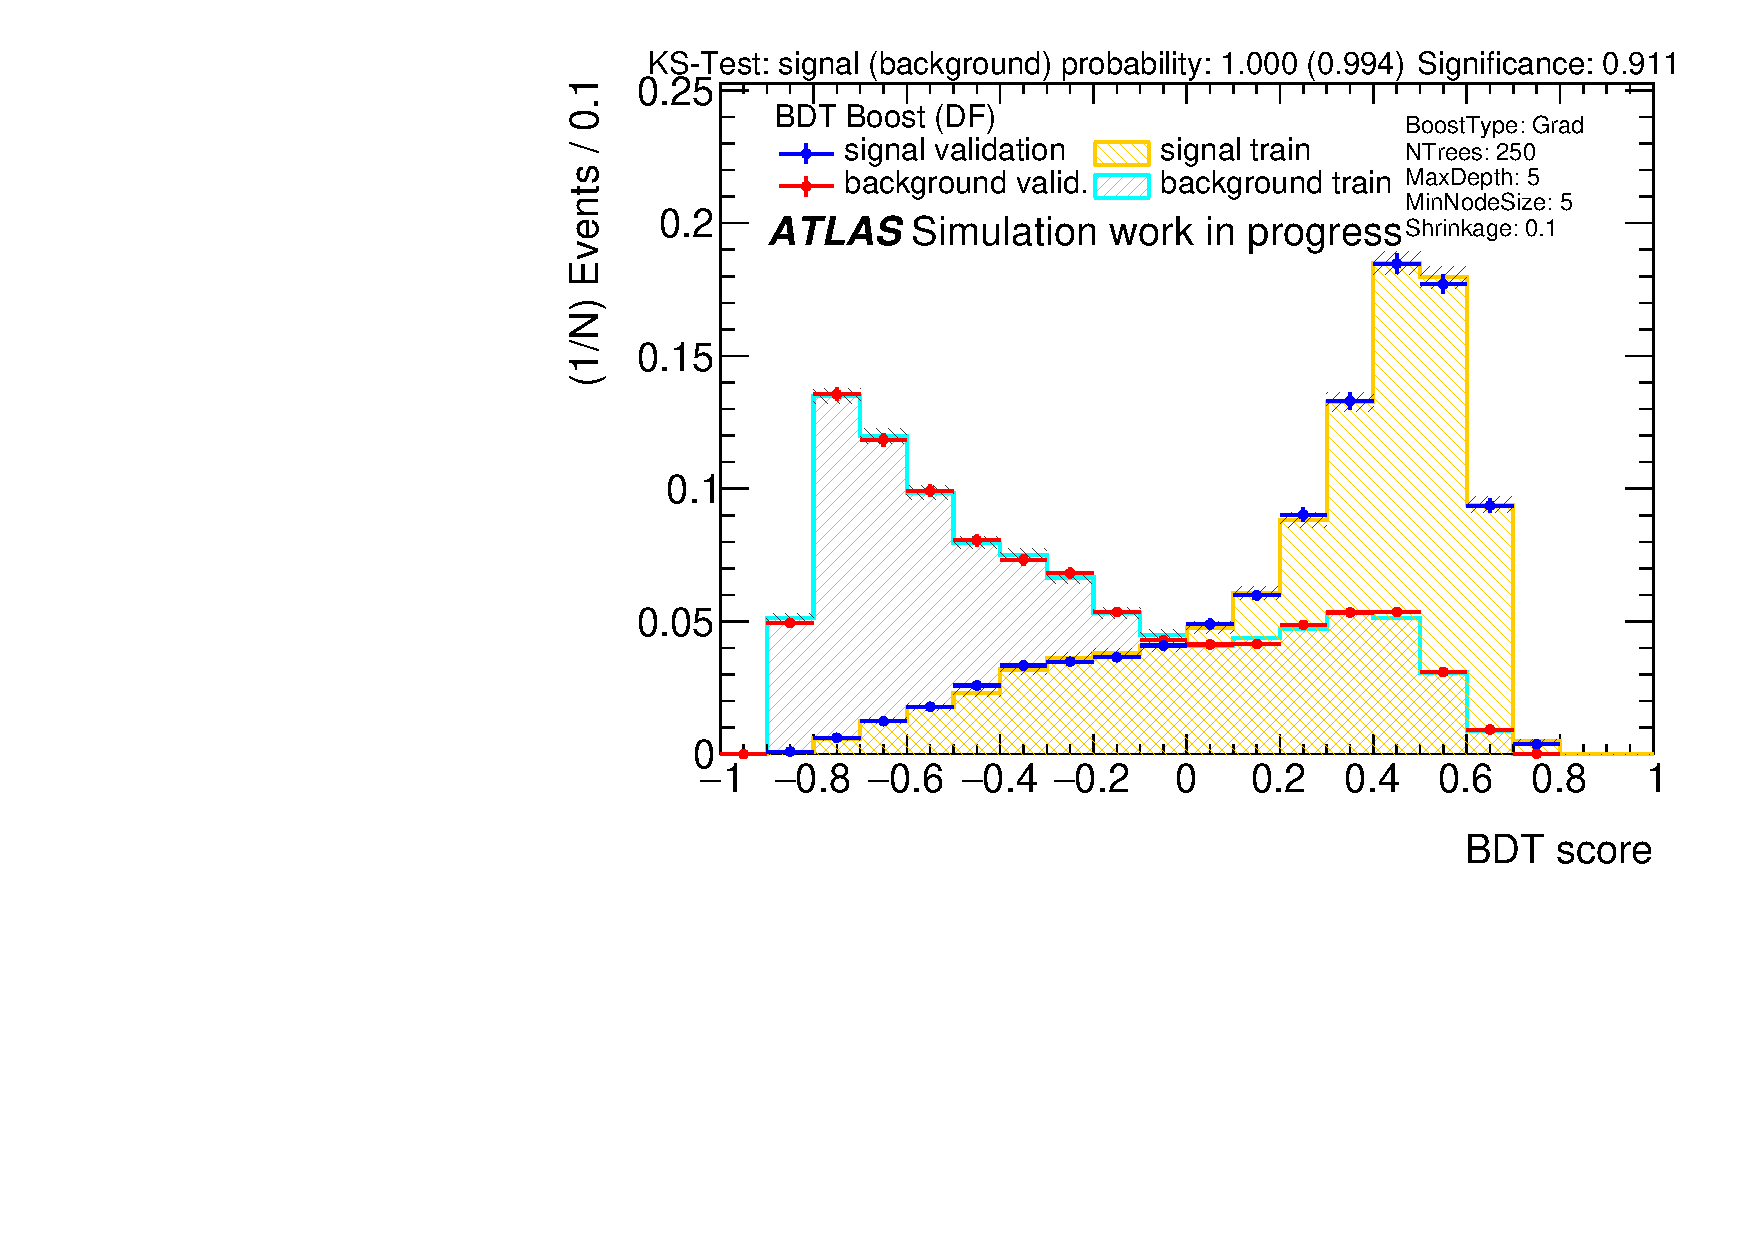
\includegraphics[width=\textwidth]{./plots/mva/variable_reduction/BOOST_DF_bdt_output_clean.pdf}
    \end{subfigure}
    \caption{Distributions of the final BDTs in the optimization of the number of input variables for signal and background and the training and validation set.
             The top row shows the BDTs for the VBF regions and the bottom row for the boosted regions.
             The same flavour regions are on the left and the different flavour regions on the right.
             The areas of all distributions are normalized to one.}~\label{fig:mva:varopt:bdts}
\end{figure}


\section{Modeling of input observables}\label{sec:mva:modeling}

It is important that there is no mismodelling of the simulated backgrounds if compared to data events.
Therefore, the modelling needs to be checked for all distributions of observables, which are used as input variables for the BDTs.
Additionally the BDT output distributions themselves need also to be checked for mismodelling.
Because the analysis is performed blinded, the full distributions of the BDT output and $\mmc$ can only be compared to data in the control regions, which
are defined in \cref{sec:background_estimation:normalization}.
In the signal regions the $\mmc$ distributions are blinded for $\SI{100}{\GeV} \leq \mmc \leq \SI{150}{\GeV}$,
and the BDT distributions are blinded for an BDT output value greater than zero.

To quantify the agreement between the background model and observed data a $\chi^2$-test is performed for all observables.
Due to the blinding this cannot be done for the $\mmc$ distribution in the signal regions.
The $\chi^2$-test probabilities are expected to follow the uniform distribution, if the predictions of the SM are correct.
Unless the $\chi^2$-test probability is tiny, i.e.\ $< 10^{-3}$, the mismodelling can be accepted, since only statistical fluctuations but
not systematic variations are considered.

\subsection{Signal region}

The distributions of the observables used in the BDT of the VBF SF region are shown in \cref{fig:mva:modeling:sr:vbfsf}.
Due to the events with large negative weights there is a large statistical fluctuation in the $\Zll$ background, which sometimes leads
to bins with an expected negative event yield and large statistical errors.
Some minor disagreement between expected background distributions and distributions of observed data can be seen for
all observables.
However, the $\chi^2$-test probabilities, which are listed in \cref{tab:mva:modeling:sr:vbf}, are still consistend with the exptectation of a flat distribution.
For the VBF DF region, the modeling is better, since there is only a very minor contribution of the $\Zll$ background.
This results in higher $\chi^2$-test probabilities.
Only the $m_\text{jj}$ distribution shows some larger mismodelling.
In the distributions of the observables used in the BDTs of the boosted categories (\cref{fig:mva:modeling:sr:boostsf,fig:mva:modeling:sr:boostdf})
generally a good agreement between simulated and observed events can be seen, except for the $\Delta R (\ell, \ell)$,
$\etmiss / \pt^{\ell_1}$, Sphericity and $\min \Delta \eta (\ell\ell, \text{jets})$ distributions.
This leads to high $\chi^2$-test probabilities, expect for the just mentioned distributions.

The distributions of the BDT output in the different signal regions are shown in \cref{fig:mva:modeling:sr:bdts}.
For the BDTs in the VBF category a good separation between signal and background is reached.
However, the background distributions of the BDTs in the boosted category start rising again for very high values
of the BDT output.
Additionally, there are two peaks in the distribution of the BDT for the boosted SF category.
Due to the large errors in the VBF SF category the background distributions agrees with the observed data within uncertainties.
A slight overshoot of simulated events can be seen in the BDT distribution of the VBF DF category.
In the BDT distributions of the boosted category the data events agree with the simulated distributions within uncertainties except for
one bin in the BDT of the boosted DF region.

\subsection{Control regions}

As a further validation, the distributions of observables and BDT outputs can also be checked in the control regions.
The modeling in the top-quark control regions (\cref{fig:mva:modeling:cr:vbftop,fig:mva:modeling:cr:boosttop})
is much better than in the $\Zll$ control regions (\cref{fig:mva:modeling:cr:vbfzll,fig:mva:modeling:cr:boostzll}).
This can also be seen in the $\chi^2$-test probabilities (\cref{tab:mva:modeling:cr:vbf,tab:mva:modeling:cr:boost}), 
where the probabilities for multiple observables are zero in the $\Zll$ control region.
The cause are again events with high negative weights in the $\Zll$ background.
However, in the statistical analysis only the yield in the control regions is used and not the shape, so
if the overall yields are modeled well this should be no major issue.
Additionally, only statistical uncertainties are considered for the $\chi^2$-test.

The distributions of the BDT output in the different control regions are shown in \cref{fig:mva:modeling:cr:bdts}.
The same trend in modeling as for the input variables can be seen.
In all these distributions the BDT output peaks at low values, which indicates that the BDTs indeed categorize
most background events correctly.

\FloatBarrier{}

\begin{table}
	\centering
    \caption{$\chi^2$-test probabilities between the background distributions of simulated events and data distributions for the observables
    used as input variables in the VBF SF and DF regions.
    Only statistical uncertainties are considered.}\label{tab:mva:modeling:sr:vbf}
	\begin{tabular}{lcc}
		\toprule
		variable & $\chi^2$ prob. SF & $\chi^2$ prob. DF \\ \midrule
		$\min \Delta \eta (\ell\ell, \text{jets})$  & 0.03 & 0.84 \\
		$m_\text{jj}$                               & 0.35 & 0.02 \\
		$\Delta R(\ell,\ell)$                       & 0.84 & 0.78 \\
		$n_\text{jets}$                             & 0.05 & 0.84 \\
		$\etmiss$ $\Phi$ centrality                 & 0.02 & 0.80 \\
		$\pt^\text{total}$                          & 0.13 & 0.28 \\
		$\etmiss$                                   & 0.87 & -- \\
		$\min \Delta R (\ell_1, \text{jets})$       & 0.10 & -- \\
		$\min \Delta R (\ell_0, \text{jets})$       & -- & 0.92 \\
		\bottomrule
	\end{tabular}
\end{table}

\begin{table}
	\centering
    \caption{$\chi^2$-test probabilities between the background distributions of simulated events and data distributions for the observables
    used as input variables in the boosted SF and DF regions.
    Only statistical uncertainties are considered.}\label{tab:mva:modeling:sr:boost}
	\begin{tabular}{lcc}
		\toprule
		variable & $\chi^2$ prob. SF & $\chi^2$ prob. DF \\ \midrule
		$m_{\ell\ell}$                              & 0.25 & 0.27 \\
		$\etmiss$                                   & 0.61 & -- \\
		$\Delta R (\ell, \ell)$                     & 0.15 & 0.02 \\
		$m_{\tau\tau,\text{j}_0} $                  & -- & 0.57 \\
		$\etmiss / \pt^{\ell_1}$                    & -- & 0.09 \\
		Sphericity                                  & -- & 0.08 \\
		$m_\text{T}^{\ell_0}$                       & -- & 0.95 \\
		$\eta_{\ell_0}$                             & -- & 0.78 \\
		$\min \Delta \eta (\ell\ell, \text{jets})$  & -- & 0.03 \\
		\bottomrule
	\end{tabular}
\end{table}

\begin{figure}[htb]
    \centering
    \begin{subfigure}[t]{0.3\textwidth}
        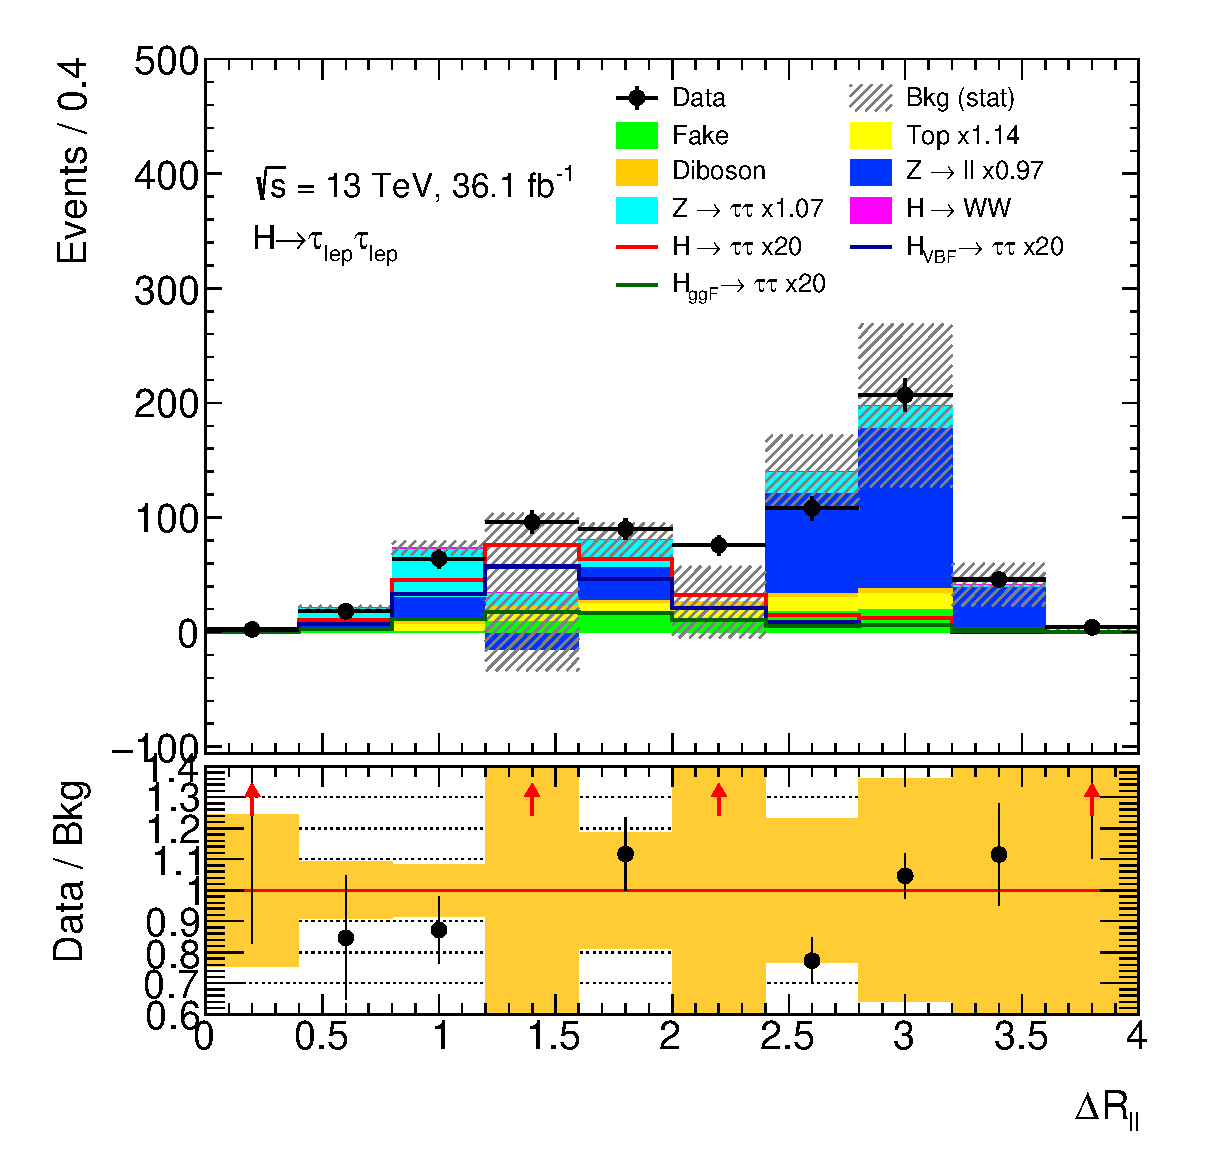
\includegraphics[width=\textwidth]{./plots/mva/modeling/input_vars/VBF_SF/ll-CutMVAVBFCatSF-DeltaRLL-lin.eps}
    \end{subfigure}
    \begin{subfigure}[t]{0.3\textwidth}
        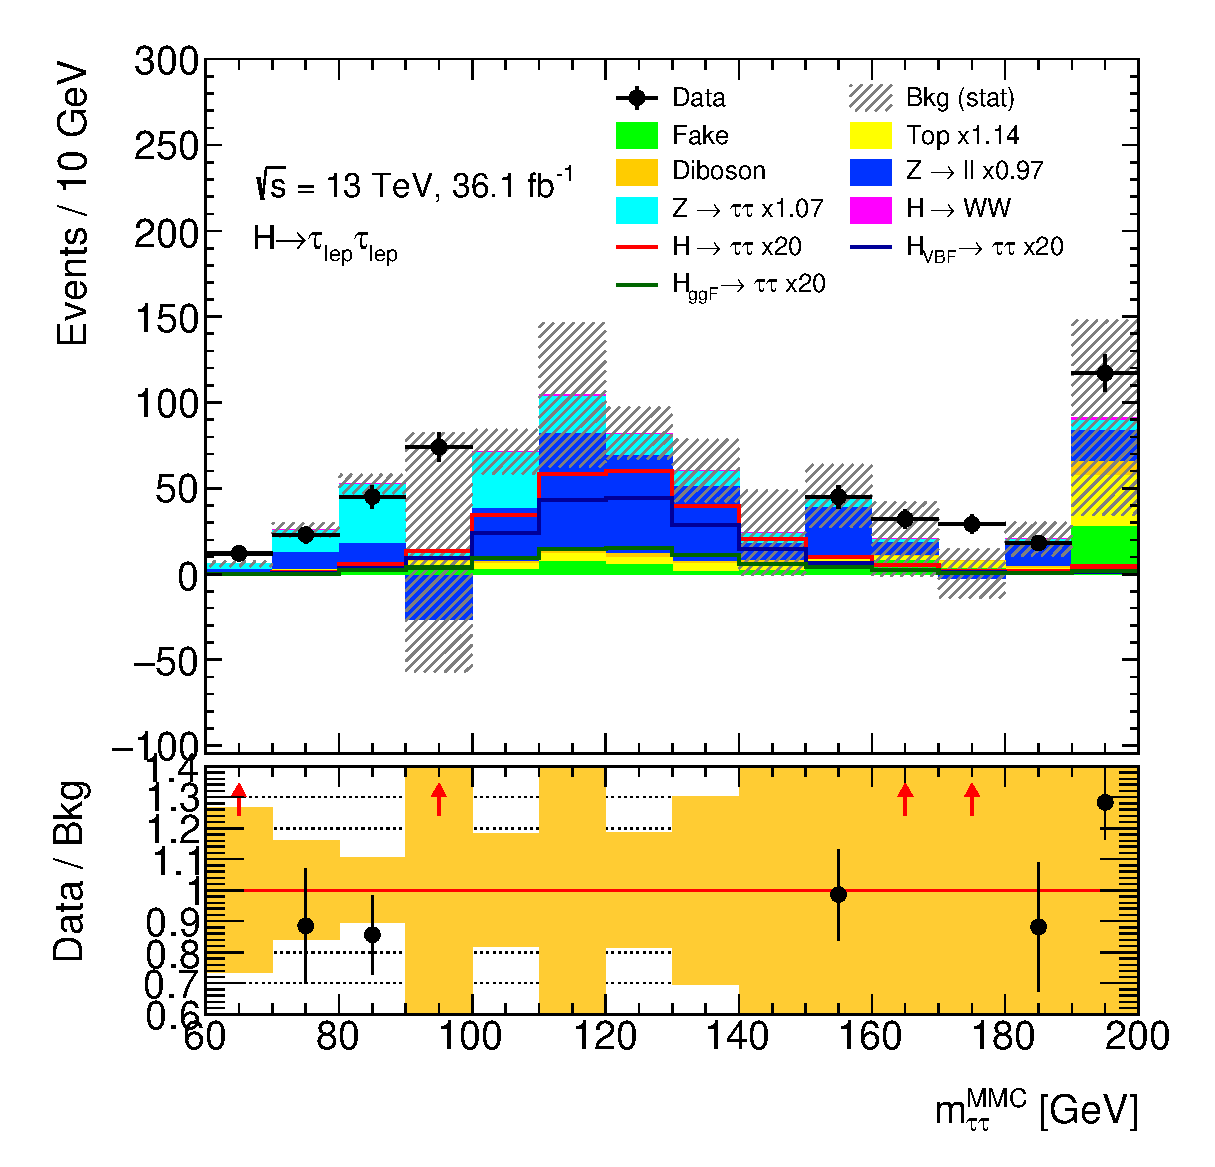
\includegraphics[width=\textwidth]{./plots/mva/modeling/input_vars/VBF_SF/ll-CutMVAVBFCatSF-dilep_mmc_mlm_m-lin.eps}
    \end{subfigure}
    \begin{subfigure}[t]{0.3\textwidth}
        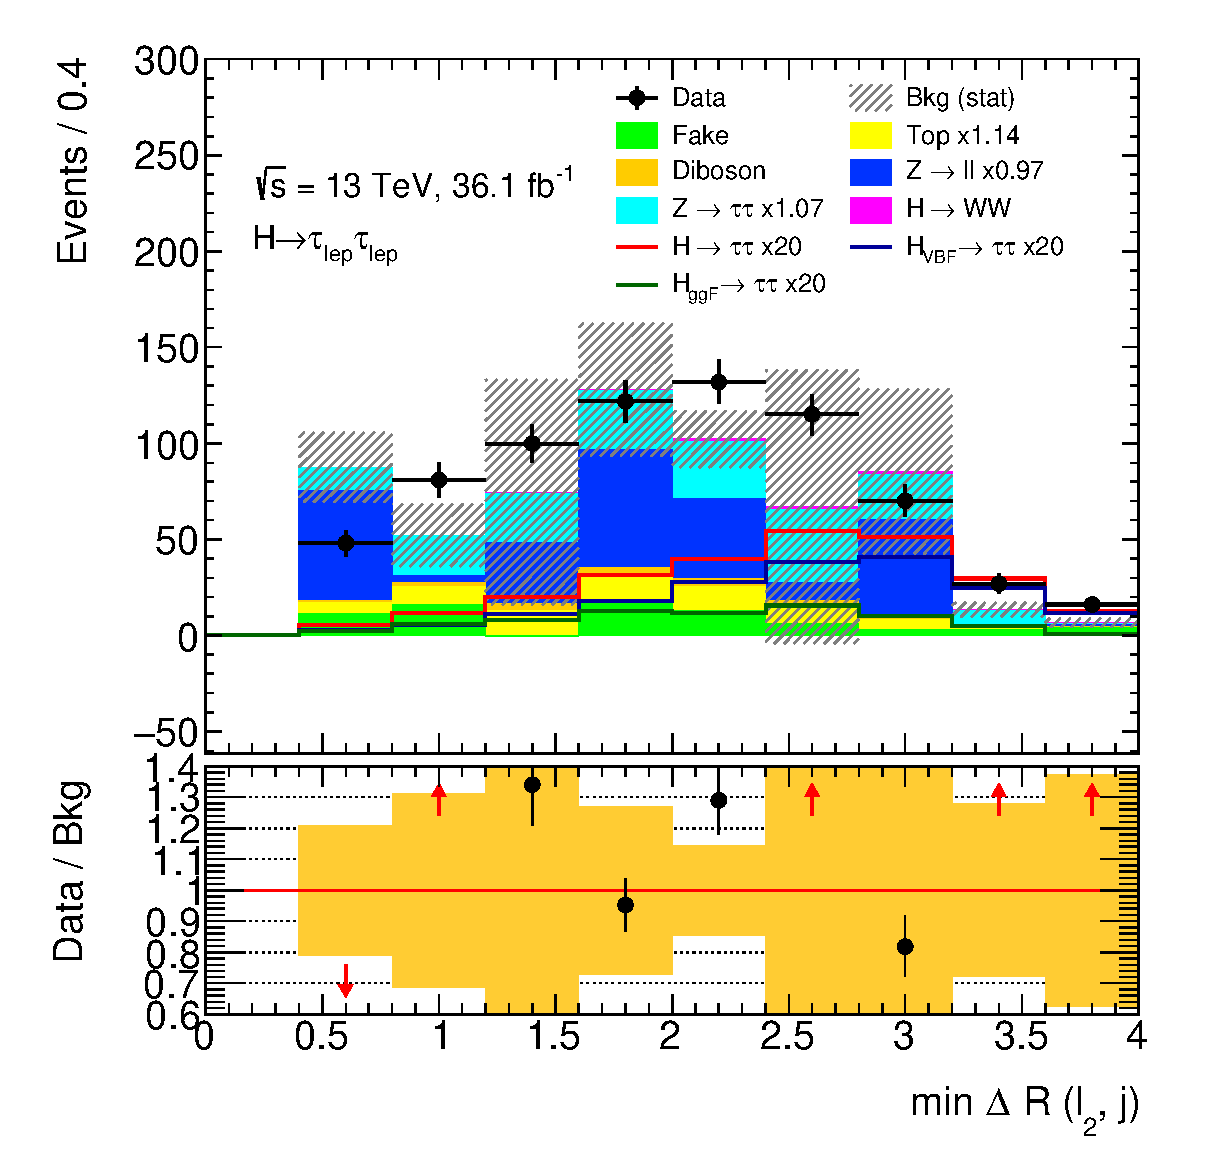
\includegraphics[width=\textwidth]{./plots/mva/modeling/input_vars/VBF_SF/ll-CutMVAVBFCatSF-dRminLep1Jet-lin.eps}
    \end{subfigure}
    \begin{subfigure}[t]{0.3\textwidth}
        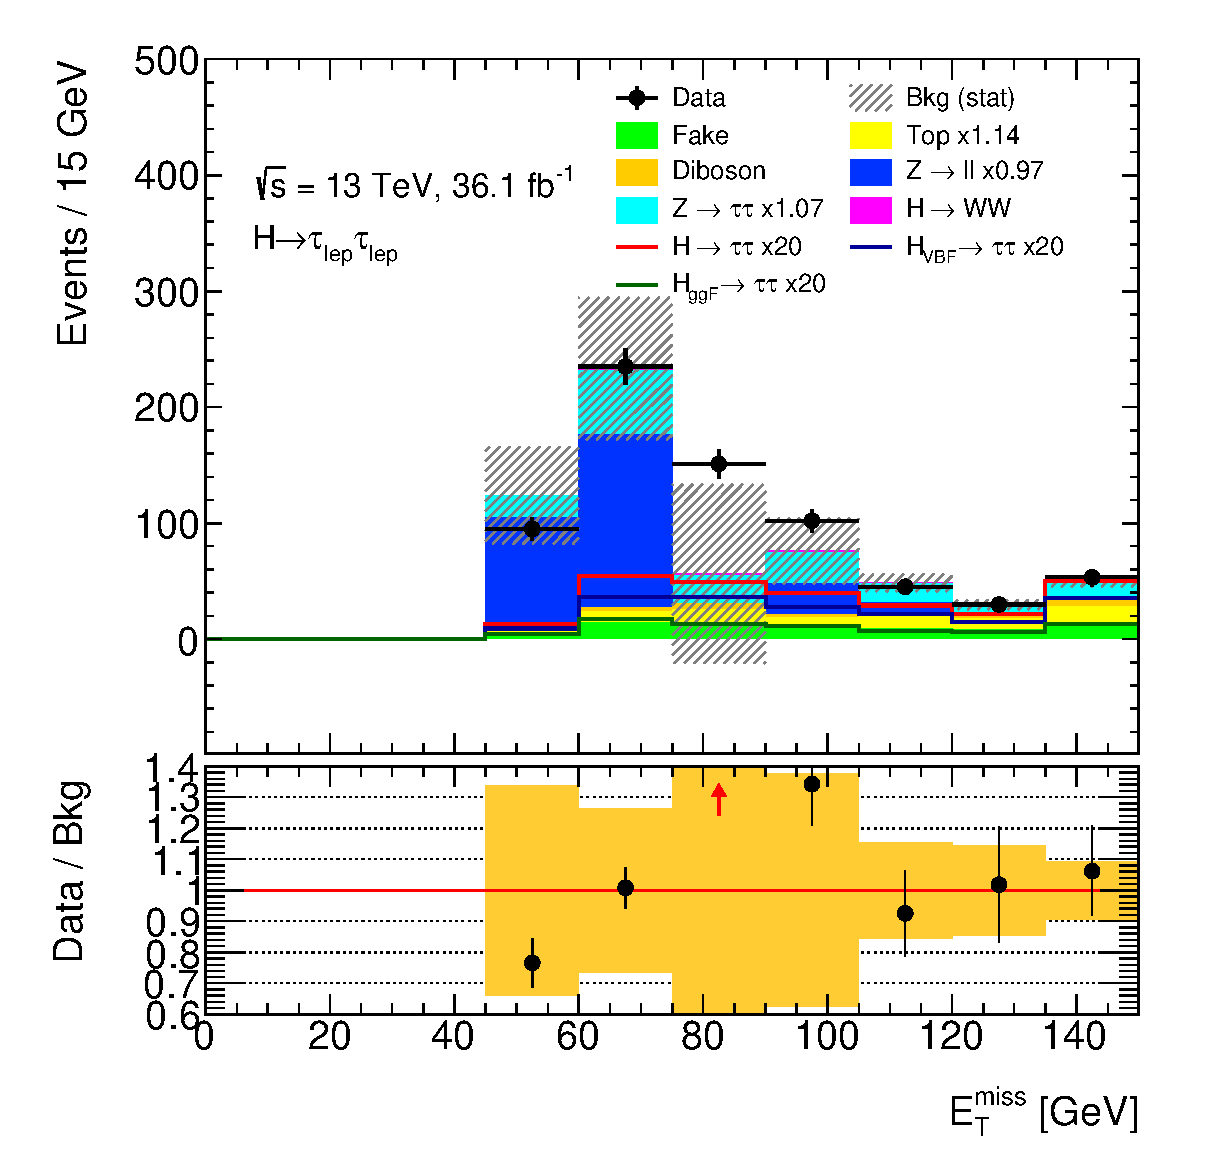
\includegraphics[width=\textwidth]{./plots/mva/modeling/input_vars/VBF_SF/ll-CutMVAVBFCatSF-MET-lin.eps}
    \end{subfigure}
    \begin{subfigure}[t]{0.3\textwidth}
        \includegraphics[width=\textwidth]{./plots/mva/modeling/input_vars/VBF_SF/ll-CutMVAVBFCatSF-METPhiCentrality2-lin.eps}
    \end{subfigure}
    \begin{subfigure}[t]{0.3\textwidth}
        \includegraphics[width=\textwidth]{./plots/mva/modeling/input_vars/VBF_SF/ll-CutMVAVBFCatSF-MinDEtaDilepJets-lin.eps}
    \end{subfigure}
    \begin{subfigure}[t]{0.3\textwidth}
        \includegraphics[width=\textwidth]{./plots/mva/modeling/input_vars/VBF_SF/ll-CutMVAVBFCatSF-Mjj-lin.eps}
    \end{subfigure}
    \begin{subfigure}[t]{0.3\textwidth}
        \includegraphics[width=\textwidth]{./plots/mva/modeling/input_vars/VBF_SF/ll-CutMVAVBFCatSF-nJets30Stacked3-lin.eps}
    \end{subfigure}
    \begin{subfigure}[t]{0.3\textwidth}
        \includegraphics[width=\textwidth]{./plots/mva/modeling/input_vars/VBF_SF/ll-CutMVAVBFCatSF-PtTotal-lin.eps}
    \end{subfigure}
    \caption{Distributions of the observables which are used as input variables for the BDTs in the VBF SF category.
             The observables are from top to bottom and from left to right: $\drll$, $\mmc$, $\min \Delta R (\ell_2, \text{jets})$,
             $\etmiss$, $\etmiss \Phi$ centrality, $\min \Delta \eta (\ell\ell, \text{jets})$, $m_{jj}$, $n_\text{jets}$, and $\pt^\text{total}$.
             The signal and background distributions are normalized to their theory cross-sections and luminosity.
             Additional normalization factors are applied on the top-quark, $\Zll$, and $\Ztautau$ background.
             The signal is scaled by a factor of 20.
             Underflow and overflow bins are included in the first and last bin, respectively.
             Only statistical uncertainties are included in the error band.}\label{fig:mva:modeling:sr:vbfsf}
\end{figure}

\begin{figure}[htb]
    \centering
    \begin{subfigure}[t]{0.3\textwidth}
        \includegraphics[width=\textwidth]{./plots/mva/modeling/input_vars/VBF_DF/ll-CutMVAVBFCatDF-DeltaRLL-lin.eps}
    \end{subfigure}
    \begin{subfigure}[t]{0.3\textwidth}
        \includegraphics[width=\textwidth]{./plots/mva/modeling/input_vars/VBF_DF/ll-CutMVAVBFCatDF-dilep_mmc_mlm_m-lin.eps}
    \end{subfigure}
    \begin{subfigure}[t]{0.3\textwidth}
        \includegraphics[width=\textwidth]{./plots/mva/modeling/input_vars/VBF_DF/ll-CutMVAVBFCatDF-dRminLep0Jet-lin.eps}
    \end{subfigure}
    \begin{subfigure}[t]{0.3\textwidth}
        \includegraphics[width=\textwidth]{./plots/mva/modeling/input_vars/VBF_DF/ll-CutMVAVBFCatDF-METPhiCentrality2-lin.eps}
    \end{subfigure}
    \begin{subfigure}[t]{0.3\textwidth}
        \includegraphics[width=\textwidth]{./plots/mva/modeling/input_vars/VBF_DF/ll-CutMVAVBFCatDF-MinDEtaDilepJets-lin.eps}
    \end{subfigure}
    \begin{subfigure}[t]{0.3\textwidth}
        \includegraphics[width=\textwidth]{./plots/mva/modeling/input_vars/VBF_DF/ll-CutMVAVBFCatDF-Mjj-lin.eps}
    \end{subfigure}
    \begin{subfigure}[t]{0.3\textwidth}
        \includegraphics[width=\textwidth]{./plots/mva/modeling/input_vars/VBF_DF/ll-CutMVAVBFCatDF-nJets30Stacked3-lin.eps}
    \end{subfigure}
    \begin{subfigure}[t]{0.3\textwidth}
        \includegraphics[width=\textwidth]{./plots/mva/modeling/input_vars/VBF_DF/ll-CutMVAVBFCatDF-PtTotal-lin.eps}
    \end{subfigure}
    \caption{Distributions of the observables which are used as input variables for the BDTs in the VBF DF category.
             The observables are from top to bottom and from left to right: $\drll$, $\mmc$, $\min \Delta R (\ell_1, \text{jets})$,
             $\etmiss \Phi$ centrality, $\min \Delta \eta (\ell\ell, \text{jets})$, $m_{jj}$, $n_\text{jets}$, and $\pt^\text{total}$.
             The signal and background distributions are normalized to their theory cross-sections and luminosity.
             Additional normalization factors are applied on the top-quark, $\Zll$, and $\Ztautau$ background.
             The signal is scaled by a factor of 20.
             Underflow and overflow bins are included in the first and last bin, respectively.
             Only statistical uncertainties are included in the error band.}\label{fig:mva:modeling:sr:vbfdf}
\end{figure}

\begin{figure}[htb]
    \centering
    \begin{subfigure}[t]{0.45\textwidth}
        \includegraphics[width=\textwidth]{./plots/mva/modeling/input_vars/BOOST_SF/ll-CutMVABoostedCatSF-DeltaRLL-lin.eps}
    \end{subfigure}
    \begin{subfigure}[t]{0.45\textwidth}
        \includegraphics[width=\textwidth]{./plots/mva/modeling/input_vars/BOOST_SF/ll-CutMVABoostedCatSF-dilep_mmc_mlm_m-lin.eps}
    \end{subfigure}
    \begin{subfigure}[t]{0.45\textwidth}
        \includegraphics[width=\textwidth]{./plots/mva/modeling/input_vars/BOOST_SF/ll-CutMVABoostedCatSF-MET-lin.eps}
    \end{subfigure}
    \begin{subfigure}[t]{0.45\textwidth}
        \includegraphics[width=\textwidth]{./plots/mva/modeling/input_vars/BOOST_SF/ll-CutMVABoostedCatSF-mvis-lin.eps}
    \end{subfigure}
    \caption{Distributions of the observables which are used as input variables for the BDTs in the boosted SF category.
             The observables are from top to bottom and from left to right: $\drll$, $\mmc$, $\etmiss$, and $\mll$.
             The signal and background distributions are normalized to their theory cross-sections and luminosity.
             Additional normalization factors are applied on the top-quark, $\Zll$, and $\Ztautau$ background.
             The signal is scaled by a factor of 20.
             Underflow and overflow bins are included in the first and last bin, respectively.
             Only statistical uncertainties are included in the error band.}\label{fig:mva:modeling:sr:boostsf}
\end{figure}

\begin{figure}[htb]
    \centering
    \begin{subfigure}[t]{0.3\textwidth}
        \includegraphics[width=\textwidth]{./plots/mva/modeling/input_vars/BOOST_DF/ll-CutMVABoostedCatDF-DeltaRLL-lin.eps}
    \end{subfigure}
    \begin{subfigure}[t]{0.3\textwidth}
        \includegraphics[width=\textwidth]{./plots/mva/modeling/input_vars/BOOST_DF/ll-CutMVABoostedCatDF-dilep_mmc_mlm_m-lin.eps}
    \end{subfigure}
    \begin{subfigure}[t]{0.3\textwidth}
        \includegraphics[width=\textwidth]{./plots/mva/modeling/input_vars/BOOST_DF/ll-CutMVABoostedCatDF-LeptonEta0-lin.eps}
    \end{subfigure}
    \begin{subfigure}[t]{0.3\textwidth}
        \includegraphics[width=\textwidth]{./plots/mva/modeling/input_vars/BOOST_DF/ll-CutMVABoostedCatDF-MassTauTauJ0-lin.eps}
    \end{subfigure}
    \begin{subfigure}[t]{0.3\textwidth}
        \includegraphics[width=\textwidth]{./plots/mva/modeling/input_vars/BOOST_DF/ll-CutMVABoostedCatDF-MinDEtaDilepJets-lin.eps}
    \end{subfigure}
    \begin{subfigure}[t]{0.3\textwidth}
        \includegraphics[width=\textwidth]{./plots/mva/modeling/input_vars/BOOST_DF/ll-CutMVABoostedCatDF-MtLep0-lin.eps}
    \end{subfigure}
    \begin{subfigure}[t]{0.3\textwidth}
        \includegraphics[width=\textwidth]{./plots/mva/modeling/input_vars/BOOST_DF/ll-CutMVABoostedCatDF-mvis-lin.eps}
    \end{subfigure}
    \begin{subfigure}[t]{0.3\textwidth}
        \includegraphics[width=\textwidth]{./plots/mva/modeling/input_vars/BOOST_DF/ll-CutMVABoostedCatDF-RatioMETPtL1-lin.eps}
    \end{subfigure}
    \begin{subfigure}[t]{0.3\textwidth}
        \includegraphics[width=\textwidth]{./plots/mva/modeling/input_vars/BOOST_DF/ll-CutMVABoostedCatDF-Sphericity-lin.eps}
    \end{subfigure}
    \caption{Distributions of the observables which are used as input variables for the BDTs in the boosted DF category.
             The observables are from top to bottom and from left to right: $\drll$, $\mmc$, $\eta_{\ell_1}$, $m_{\tau\tau,j_{1}}$,
             $\min \Delta \eta (\ell, \text{jets})$, $m_\text{T}^{\ell_1}$, $\mll$, $\etmiss / \pt^{\ell_2}$, and Sphericity.
             The signal and background distributions are normalized to their theory cross-sections and luminosity.
             Additional normalization factors are applied on the top-quark, $\Zll$, and $\Ztautau$ background.
             The signal is scaled by a factor of 20.
             Underflow and overflow bins are included in the first and last bin, respectively.
             Only statistical uncertainties are included in the error band.}\label{fig:mva:modeling:sr:boostdf}
\end{figure}

\begin{figure}[htb]
    \centering
    \begin{subfigure}[t]{0.45\textwidth}
        \includegraphics[width=\textwidth]{./plots/mva/modeling/BDT/SR/eemm-CutMVAVBFCatSF-BDT_VBF_SF-lin.eps}
    \end{subfigure}
    \begin{subfigure}[t]{0.45\textwidth}
        \includegraphics[width=\textwidth]{./plots/mva/modeling/BDT/SR/emme-CutMVAVBFCatDF-BDT_VBF_DF-lin.eps}
    \end{subfigure}
    \begin{subfigure}[t]{0.45\textwidth}
        \includegraphics[width=\textwidth]{./plots/mva/modeling/BDT/SR/eemm-CutMVABoostedCatSF-BDT_BOOST_SF-lin.eps}
    \end{subfigure}
    \begin{subfigure}[t]{0.45\textwidth}
        \includegraphics[width=\textwidth]{./plots/mva/modeling/BDT/SR/emme-CutMVABoostedCatDF-BDT_BOOST_DF-lin.eps}
    \end{subfigure}
    \caption{Distributions of BDT outputs in the VBF SF (top left), VBF DF (top right), boosted SF (bottom left), and boosted DF (bottom right) region.
             The signal and background distributions are normalized to their theory cross-sections and luminosity.
             Additional normalization factors are applied on the top-quark, $\Zll$, and $\Ztautau$ background.
             The signal is scaled by a factor of 20.
             Underflow and overflow bins are included in the first and last bin, respectively.
             Only statistical uncertainties are included in the error band.}\label{fig:mva:modeling:sr:bdts}
\end{figure}

\begin{table}
	\centering
    \caption{$\chi^2$-test probabilities between the background distributions in the control regions for the VBF category of simulated events and data distributions for the observables
    used as input variables in the VBF SF and DF regions.
    Only statistical uncertainties are considered.}\label{tab:mva:modeling:cr:vbf}
	\begin{tabular}{lcc}
		\toprule
		variable & $\chi^2$ prob. Zll CR & $\chi^2$ prob. Top CR \\ \midrule
		$m_\text{MMC}^\text{mlm}$                   & 0.00 & 0.62 \\
		$\min \Delta \eta (\ell\ell, \text{jets})$  & 0.14 & 0.95 \\
		$m_\text{jj}$                               & 0.00 & 0.31 \\
		$\Delta R(\ell,\ell)$                       & 0.55 & 0.06 \\
		$n_\text{jets}$                             & 0.00 & 0.34 \\
		$\etmiss$ $\Phi$ centrality                 & 0.19 & 0.57 \\
		$\pt^\text{total}$                          & 0.00 & 0.08 \\
		$\etmiss$                                   & 0.00 & 0.19 \\
		$\min \Delta R (\ell_0, \text{jets})$       & 0.13 & 0.08 \\
		$\min \Delta R (\ell_1, \text{jets})$       & 0.14 & 0.18 \\
		\bottomrule
	\end{tabular}
\end{table}

\begin{table}
	\centering
    \caption{$\chi^2$-test probabilities between the background distributions in the control regions for the boosted category of simulated events and data distributions for the observables
    used as input variables in the boosted SF and DF regions.
    Only statistical uncertainties are considered.}\label{tab:mva:modeling:cr:boost}
	\begin{tabular}{lcc}
		\toprule
		variable & $\chi^2$ prob. Zll CR & $\chi^2$ prob. Top CR \\ \midrule
		$m_\text{MMC}^\text{mlm}$                   & 0.00 & 0.16 \\
		$m_{\ell\ell}$                              & 0.14 & 0.47 \\
		$\etmiss$                                   & 0.00 & 0.20 \\
		$\Delta R (\ell, \ell)$                     & 0.00 & 0.06 \\
		$m_{\tau\tau,\text{j}_0} $                  & 0.06 & 0.71 \\
		$\etmiss / \pt^{\ell_1}$                    & 0.00 & 0.22 \\
		sphericity                                  & 0.50 & 0.17 \\
		$m_\text{T}^{\ell_0}$                       & 0.00 & 0.13 \\
		$\eta_{\ell_0}$                             & 0.13 & 0.12 \\
		$\min \Delta \eta (\ell\ell, \text{jets})$  & 0.10 & 0.55 \\
		\bottomrule
	\end{tabular}
\end{table}


\begin{figure}[htb]
    \centering
    \begin{subfigure}[t]{0.3\textwidth}
        \includegraphics[width=\textwidth]{./plots/mva/modeling/input_vars/VBF_CR/ll-CutMVAVBFCatTopCR-DeltaRLL-lin.eps}
    \end{subfigure}
    \begin{subfigure}[t]{0.3\textwidth}
        \includegraphics[width=\textwidth]{./plots/mva/modeling/input_vars/VBF_CR/ll-CutMVAVBFCatTopCR-dilep_mmc_mlm_m_ub-lin.eps}
    \end{subfigure}
    \begin{subfigure}[t]{0.3\textwidth}
        \includegraphics[width=\textwidth]{./plots/mva/modeling/input_vars/VBF_CR/ll-CutMVAVBFCatTopCR-dRminLep0Jet-lin.eps}
    \end{subfigure}
    \begin{subfigure}[t]{0.3\textwidth}
        \includegraphics[width=\textwidth]{./plots/mva/modeling/input_vars/VBF_CR/ll-CutMVAVBFCatTopCR-dRminLep1Jet-lin.eps}
    \end{subfigure}
    \begin{subfigure}[t]{0.3\textwidth}
        \includegraphics[width=\textwidth]{./plots/mva/modeling/input_vars/VBF_CR/ll-CutMVAVBFCatTopCR-MET-lin.eps}
    \end{subfigure}
    \begin{subfigure}[t]{0.3\textwidth}
        \includegraphics[width=\textwidth]{./plots/mva/modeling/input_vars/VBF_CR/ll-CutMVAVBFCatTopCR-METPhiCentrality2-lin.eps}
    \end{subfigure}
    \begin{subfigure}[t]{0.3\textwidth}
        \includegraphics[width=\textwidth]{./plots/mva/modeling/input_vars/VBF_CR/ll-CutMVAVBFCatTopCR-MinDEtaDilepJets-lin.eps}
    \end{subfigure}
    \begin{subfigure}[t]{0.3\textwidth}
        \includegraphics[width=\textwidth]{./plots/mva/modeling/input_vars/VBF_CR/ll-CutMVAVBFCatTopCR-Mjj-lin.eps}
    \end{subfigure}
    \begin{subfigure}[t]{0.3\textwidth}
        \includegraphics[width=\textwidth]{./plots/mva/modeling/input_vars/VBF_CR/ll-CutMVAVBFCatTopCR-nJets30Stacked3-lin.eps}
    \end{subfigure}
    \begin{subfigure}[t]{0.3\textwidth}
        \includegraphics[width=\textwidth]{./plots/mva/modeling/input_vars/VBF_CR/ll-CutMVAVBFCatTopCR-PtTotal-lin.eps}
    \end{subfigure}
    \caption{Distributions of the observables which are used as input variables for the VBF SF and VBF DF BDTs in the top-quark control region.
             The observables are from top to bottom and from left to right: $\drll$, $\mmc$, $\min \Delta R (\ell_1, \text{jets})$, $\min \Delta R (\ell_2, \text{jets})$,
             $\etmiss$, $\etmiss \Phi$ centrality, $\min \Delta \eta (\ell\ell, \text{jets})$, $m_{jj}$, $n_\text{jets}$, and $\pt^\text{total}$.
             The signal and background distributions are normalized to their theory cross-sections and luminosity.
             Additional normalization factors are applied on the top-quark, $\Zll$, and $\Ztautau$ background.
             The signal is scaled by a factor of 20.
             Underflow and overflow bins are included in the first and last bin, respectively.
             Only statistical uncertainties are included in the error band.}\label{fig:mva:modeling:cr:vbftop}
\end{figure}

\begin{figure}[htb]
    \centering
    \begin{subfigure}[t]{0.3\textwidth}
        \includegraphics[width=\textwidth]{./plots/mva/modeling/input_vars/VBF_CR/ll-CutMVAVBFCatZllCR-DeltaRLL-lin.eps}
    \end{subfigure}
    \begin{subfigure}[t]{0.3\textwidth}
        \includegraphics[width=\textwidth]{./plots/mva/modeling/input_vars/VBF_CR/ll-CutMVAVBFCatZllCR-dilep_mmc_mlm_m_ub-lin.eps}
    \end{subfigure}
    \begin{subfigure}[t]{0.3\textwidth}
        \includegraphics[width=\textwidth]{./plots/mva/modeling/input_vars/VBF_CR/ll-CutMVAVBFCatZllCR-dRminLep0Jet-lin.eps}
    \end{subfigure}
    \begin{subfigure}[t]{0.3\textwidth}
        \includegraphics[width=\textwidth]{./plots/mva/modeling/input_vars/VBF_CR/ll-CutMVAVBFCatZllCR-dRminLep1Jet-lin.eps}
    \end{subfigure}
    \begin{subfigure}[t]{0.3\textwidth}
        \includegraphics[width=\textwidth]{./plots/mva/modeling/input_vars/VBF_CR/ll-CutMVAVBFCatZllCR-MET-lin.eps}
    \end{subfigure}
    \begin{subfigure}[t]{0.3\textwidth}
        \includegraphics[width=\textwidth]{./plots/mva/modeling/input_vars/VBF_CR/ll-CutMVAVBFCatZllCR-METPhiCentrality2-lin.eps}
    \end{subfigure}
    \begin{subfigure}[t]{0.3\textwidth}
        \includegraphics[width=\textwidth]{./plots/mva/modeling/input_vars/VBF_CR/ll-CutMVAVBFCatZllCR-MinDEtaDilepJets-lin.eps}
    \end{subfigure}
    \begin{subfigure}[t]{0.3\textwidth}
        \includegraphics[width=\textwidth]{./plots/mva/modeling/input_vars/VBF_CR/ll-CutMVAVBFCatZllCR-Mjj-lin.eps}
    \end{subfigure}
    \begin{subfigure}[t]{0.3\textwidth}
        \includegraphics[width=\textwidth]{./plots/mva/modeling/input_vars/VBF_CR/ll-CutMVAVBFCatZllCR-nJets30Stacked3-lin.eps}
    \end{subfigure}
    \begin{subfigure}[t]{0.3\textwidth}
        \includegraphics[width=\textwidth]{./plots/mva/modeling/input_vars/VBF_CR/ll-CutMVAVBFCatZllCR-PtTotal-lin.eps}
    \end{subfigure}
    \caption{Distributions of the observables which are used as input variables for the VBF SF and VBF DF BDTs in the $\Zll$ control region.
             The observables are from top to bottom and from left to right: $\drll$, $\mmc$, $\min \Delta R (\ell_1, \text{jets})$, $\min \Delta R (\ell_2, \text{jets})$,
             $\etmiss$, $\etmiss \Phi$ centrality, $\min \Delta \eta (\ell\ell, \text{jets})$, $m_{jj}$, $n_\text{jets}$, and $\pt^\text{total}$.
             The signal and background distributions are normalized to their theory cross-sections and luminosity.
             Additional normalization factors are applied on the top-quark, $\Zll$, and $\Ztautau$ background.
             The signal is scaled by a factor of 20.
             Underflow and overflow bins are included in the first and last bin, respectively.
             Only statistical uncertainties are included in the error band.}\label{fig:mva:modeling:cr:vbfzll}
\end{figure}

\begin{figure}[htb]
    \centering
    \begin{subfigure}[t]{0.3\textwidth}
        \includegraphics[width=\textwidth]{./plots/mva/modeling/input_vars/BOOST_CR/ll-CutMVABoostedCatTopCR-DeltaRLL-lin.eps}
    \end{subfigure}
    \begin{subfigure}[t]{0.3\textwidth}
        \includegraphics[width=\textwidth]{./plots/mva/modeling/input_vars/BOOST_CR/ll-CutMVABoostedCatTopCR-dilep_mmc_mlm_m_ub-lin.eps}
    \end{subfigure}
    \begin{subfigure}[t]{0.3\textwidth}
        \includegraphics[width=\textwidth]{./plots/mva/modeling/input_vars/BOOST_CR/ll-CutMVABoostedCatTopCR-LeptonEta0-lin.eps}
    \end{subfigure}
    \begin{subfigure}[t]{0.3\textwidth}
        \includegraphics[width=\textwidth]{./plots/mva/modeling/input_vars/BOOST_CR/ll-CutMVABoostedCatTopCR-MET-lin.eps}
    \end{subfigure}
    \begin{subfigure}[t]{0.3\textwidth}
        \includegraphics[width=\textwidth]{./plots/mva/modeling/input_vars/BOOST_CR/ll-CutMVABoostedCatTopCR-MassTauTauJ0-lin.eps}
    \end{subfigure}
    \begin{subfigure}[t]{0.3\textwidth}
        \includegraphics[width=\textwidth]{./plots/mva/modeling/input_vars/BOOST_CR/ll-CutMVABoostedCatTopCR-MinDEtaDilepJets-lin.eps}
    \end{subfigure}
    \begin{subfigure}[t]{0.3\textwidth}
        \includegraphics[width=\textwidth]{./plots/mva/modeling/input_vars/BOOST_CR/ll-CutMVABoostedCatTopCR-MtLep0-lin.eps}
    \end{subfigure}
    \begin{subfigure}[t]{0.3\textwidth}
        \includegraphics[width=\textwidth]{./plots/mva/modeling/input_vars/BOOST_CR/ll-CutMVABoostedCatTopCR-mvis-lin.eps}
    \end{subfigure}
    \begin{subfigure}[t]{0.3\textwidth}
        \includegraphics[width=\textwidth]{./plots/mva/modeling/input_vars/BOOST_CR/ll-CutMVABoostedCatTopCR-RatioMETPtL1-lin.eps}
    \end{subfigure}
    \begin{subfigure}[t]{0.3\textwidth}
        \includegraphics[width=\textwidth]{./plots/mva/modeling/input_vars/BOOST_CR/ll-CutMVABoostedCatTopCR-Sphericity-lin.eps}
    \end{subfigure}
    \caption{Distributions of the observables which are used as input variables for the boosted SF and boosted DF BDTs in the top-quark control region.
             The observables are from top to bottom and from left to right: $\drll$, $\mmc$, $\eta_{\ell_1}$, $\etmiss$, $m_{\tau\tau,j_{1}}$,
             $\min \Delta \eta (\ell, \text{jets})$, $m_\text{T}^{\ell_1}$, $\mll$, $\etmiss / \pt^{\ell_2}$, and Sphericity.
             The signal and background distributions are normalized to their theory cross-sections and luminosity.
             Additional normalization factors are applied on the top-quark, $\Zll$, and $\Ztautau$ background.
             The signal is scaled by a factor of 20.
             Underflow and overflow bins are included in the first and last bin, respectively.
             Only statistical uncertainties are included in the error band.}\label{fig:mva:modeling:cr:boosttop}
\end{figure}

\begin{figure}[htb]
    \centering
    \begin{subfigure}[t]{0.3\textwidth}
        \includegraphics[width=\textwidth]{./plots/mva/modeling/input_vars/BOOST_CR/ll-CutMVABoostedCatZllCR-DeltaRLL-lin.eps}
    \end{subfigure}
    \begin{subfigure}[t]{0.3\textwidth}
        \includegraphics[width=\textwidth]{./plots/mva/modeling/input_vars/BOOST_CR/ll-CutMVABoostedCatZllCR-dilep_mmc_mlm_m_ub-lin.eps}
    \end{subfigure}
    \begin{subfigure}[t]{0.3\textwidth}
        \includegraphics[width=\textwidth]{./plots/mva/modeling/input_vars/BOOST_CR/ll-CutMVABoostedCatZllCR-LeptonEta0-lin.eps}
    \end{subfigure}
    \begin{subfigure}[t]{0.3\textwidth}
        \includegraphics[width=\textwidth]{./plots/mva/modeling/input_vars/BOOST_CR/ll-CutMVABoostedCatZllCR-MET-lin.eps}
    \end{subfigure}
    \begin{subfigure}[t]{0.3\textwidth}
        \includegraphics[width=\textwidth]{./plots/mva/modeling/input_vars/BOOST_CR/ll-CutMVABoostedCatZllCR-MassTauTauJ0-lin.eps}
    \end{subfigure}
    \begin{subfigure}[t]{0.3\textwidth}
        \includegraphics[width=\textwidth]{./plots/mva/modeling/input_vars/BOOST_CR/ll-CutMVABoostedCatZllCR-MinDEtaDilepJets-lin.eps}
    \end{subfigure}
    \begin{subfigure}[t]{0.3\textwidth}
        \includegraphics[width=\textwidth]{./plots/mva/modeling/input_vars/BOOST_CR/ll-CutMVABoostedCatZllCR-MtLep0-lin.eps}
    \end{subfigure}
    \begin{subfigure}[t]{0.3\textwidth}
        \includegraphics[width=\textwidth]{./plots/mva/modeling/input_vars/BOOST_CR/ll-CutMVABoostedCatZllCR-mvis2-lin.eps}
    \end{subfigure}
    \begin{subfigure}[t]{0.3\textwidth}
        \includegraphics[width=\textwidth]{./plots/mva/modeling/input_vars/BOOST_CR/ll-CutMVABoostedCatZllCR-RatioMETPtL1-lin.eps}
    \end{subfigure}
    \begin{subfigure}[t]{0.3\textwidth}
        \includegraphics[width=\textwidth]{./plots/mva/modeling/input_vars/BOOST_CR/ll-CutMVABoostedCatZllCR-Sphericity-lin.eps}
    \end{subfigure}
    \caption{Distributions of the observables which are used as input variables for the boosted SF and boosted DF BDTs in the $\Zll$ control region.
             The observables are from top to bottom and from left to right: $\drll$, $\mmc$, $\eta_{\ell_1}$, $\etmiss$, $m_{\tau\tau,j_{1}}$,
             $\min \Delta \eta (\ell, \text{jets})$, $m_\text{T}^{\ell_1}$, $\mll$, $\etmiss / \pt^{\ell_2}$, and Sphericity.
             The signal and background distributions are normalized to their theory cross-sections and luminosity.
             Additional normalization factors are applied on the top-quark, $\Zll$, and $\Ztautau$ background.
             The signal is scaled by a factor of 20.
             Underflow and overflow bins are included in the first and last bin, respectively.
             Only statistical uncertainties are included in the error band.}\label{fig:mva:modeling:cr:boostzll}
\end{figure}

\begin{figure}[htb]
    \centering
    \begin{subfigure}[t]{0.45\textwidth}
        \includegraphics[width=\textwidth]{./plots/mva/modeling/BDT/CRs/eemm-CutMVAVBFCatTopCR-BDT_VBF_CR-lin.eps}
    \end{subfigure}
    \begin{subfigure}[t]{0.45\textwidth}
        \includegraphics[width=\textwidth]{./plots/mva/modeling/BDT/CRs/emme-CutMVAVBFCatTopCR-BDT_VBF_CR-lin.eps}
    \end{subfigure}
    \begin{subfigure}[t]{0.45\textwidth}
        \includegraphics[width=\textwidth]{./plots/mva/modeling/BDT/CRs/eemm-CutMVABoostedCatTopCR-BDT_BOOST_CR-lin.eps}
    \end{subfigure}
    \begin{subfigure}[t]{0.45\textwidth}
        \includegraphics[width=\textwidth]{./plots/mva/modeling/BDT/CRs/emme-CutMVABoostedCatTopCR-BDT_BOOST_CR-lin.eps}
    \end{subfigure}
    \begin{subfigure}[t]{0.45\textwidth}
        \includegraphics[width=\textwidth]{./plots/mva/modeling/BDT/CRs/eemm-CutMVAVBFCatZllCR-BDT_VBF_CR-lin.eps}
    \end{subfigure}
    \begin{subfigure}[t]{0.45\textwidth}
        \includegraphics[width=\textwidth]{./plots/mva/modeling/BDT/CRs/eemm-CutMVABoostedCatZllCR-BDT_BOOST_CR-lin.eps}
    \end{subfigure}
    \caption{Distributions of BDT outputs in the top-quark control region (VBF SF:\ top left, VBF DF:\ top right, boosted SF:\ center left, boosted DF:\ center right)
             and $\Zll$ control region (VBF SF:\ bottom left, boosted SF\: bottom right).
             The signal and background distributions are normalized to their theory cross-sections and luminosity.
             Additional normalization factors are applied on the top-quark, $\Zll$, and $\Ztautau$ background.
             The signal is scaled by a factor of 20.
             Underflow and overflow bins are included in the first and last bin, respectively.
             Only statistical uncertainties are included in the error band.}\label{fig:mva:modeling:cr:bdts}
\end{figure}

